\subsection{1D dataset of GLOBAL\_MEAN\_ATM\_SURFACE\_PRES}
\newp
\subsubsection{Overview}
This dataset provides a 1D field of global mean atmospheric surface pressure over the ocean and sea-ice from the ECCO Version 4 Release 4 (V4r4) ocean and sea-ice state estimate. The dataset is provided on instantaneous hourly, daily-average and monthly-average time resolution. 
\begin{longtable}{|m{0.15\textwidth}|m{0.64\textwidth}|m{0.12\textwidth}|}
\caption{Coordinates and Variables in the dataset GLOBAL\_MEAN\_ATM\_SURFACE\_PRES}
\label{tab:table-GLOBAL_MEAN_ATM_SURFACE_PRES-fields} \\ 
\hline \endhead \hline \endfoot
\rowcolor{lightgray} \multicolumn{1}{|c|}{\textbf{Coordinates}} & \multicolumn{1}{|c|}{\textbf{Description of data coordinates}} &  \multicolumn{1}{|c|}{\textbf{Unit}}\\ \hline
time &Snapshot time &--none--  \\ \hline
\rowcolor{lightgray} \multicolumn{1}{|c|}{\textbf{Variables}} & \multicolumn{1}{|c|}{\textbf{Description of data variables}} &  \multicolumn{1}{|c|}{\textbf{Unit}}\\ \hline
Pa\_global &Global mean atmospheric surface pressure over the ocean and sea-ice &N m-2  \\ \hline
\end{longtable}

\newp
\pagebreak
\subsubsection{1D Variable: Pa\_global}
\begin{longtable}{|m{0.06\textwidth}|m{0.3\textwidth}|m{0.45\textwidth}|m{0.12\textwidth}|}
\caption{Attributes description of the variable 'Pa\_global' from GLOBAL\_MEAN\_ATM\_SURFACE\_PRES's  dataset.}
\label{tab:table-GLOBAL_MEAN_ATM_SURFACE_PRES_Pa_global} \\ 
\hline \endhead \hline \endfoot
\rowcolor{lightgray} \textbf{Storage Type} & \textbf{Variable Name} & \textbf{Description} & \textbf{Unit} \\ \hline
float64 & Pa\_global & Global mean atmospheric surface pressure over the ocean and sea-ice & N m-2 \\ \hline
\multicolumn{4}{|c|}{\cellcolor{lightgray}{\textbf{Description of the variable in Common Data language (CDL)}}} \\ \hline
\multicolumn{4}{|c|}{\fontfamily{lmtt}\selectfont{\makecell{\parbox{.95\textwidth}{\vspace*{0.25cm} \footnotesize{float64 Pa\_global(time)\\
\hspace*{0.5cm}Pa\_global: \_FillValue = 9.969209968386869e+36\\
\hspace*{0.5cm}Pa\_global: coordinates = time\\
\hspace*{0.5cm}Pa\_global: coverage\_content\_type = modelResult\\
\hspace*{0.5cm}Pa\_global: long\_name = Global mean atmospheric surface pressure over the ocean and sea-ice\\
\hspace*{0.5cm}Pa\_global: standard\_name = air pressure at sea level\\
\hspace*{0.5cm}Pa\_global: units = N m-2\\
\hspace*{0.5cm}Pa\_global: valid\_max = 101257.45252296235\\
\hspace*{0.5cm}Pa\_global: valid\_min = 100873.14755283327\\
}}}}} \\ \hline
\rowcolor{lightgray} \multicolumn{4}{|c|}{\textbf{Comments}} \\ \hline
\multicolumn{4}{|p{1\textwidth}|}{\footnotesize{{N/a}}} \\ \hline
\end{longtable}

\begin{figure}[H]
\centering
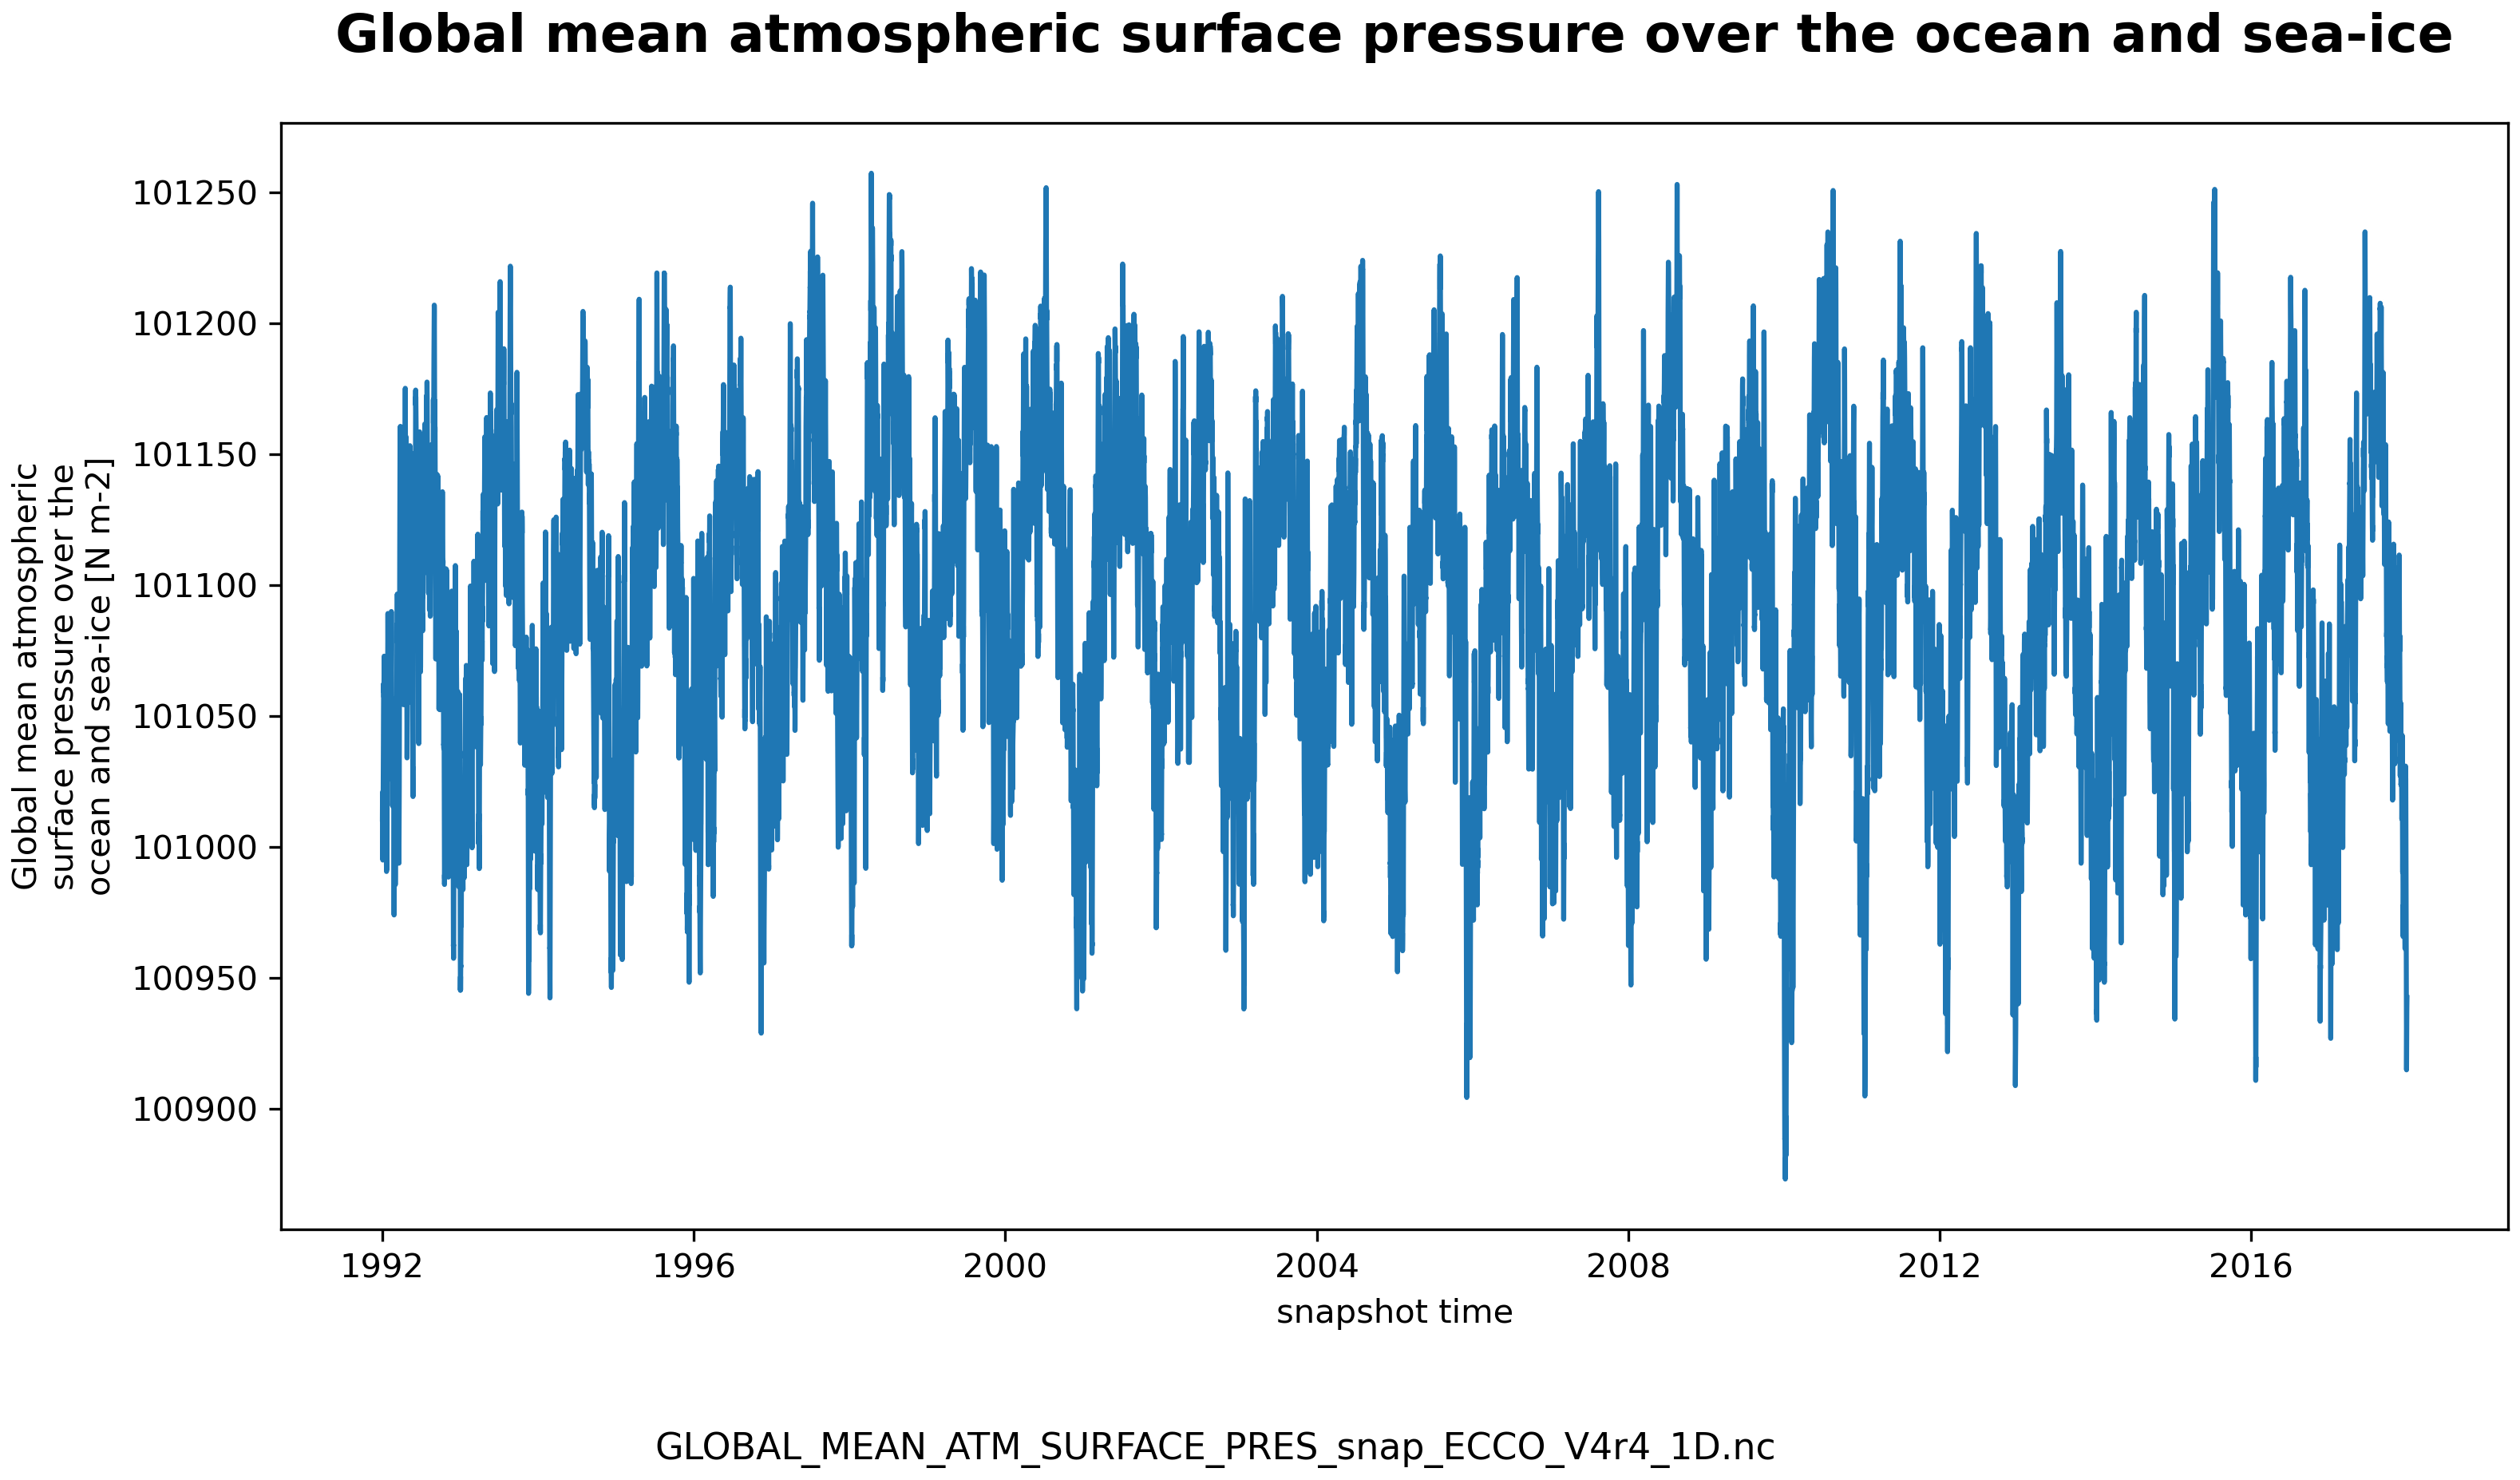
\includegraphics[scale=0.55]{../images/plots/v4r4/oneD_plots/Global_Mean_Atmospheric_Pressure/Pa_global.png}
\caption{Dataset: GLOBAL\_MEAN\_ATM\_SURFACE\_PRES, Variable: Pa\_global}
\label{tab:table-GLOBAL_MEAN_ATM_SURFACE_PRES_Pa_global-Plot}
\end{figure}
\newpage
\subsection{1D dataset of GLOBAL\_MEAN\_SEA\_LEVEL}
\newp
\subsubsection{Overview}
This dataset provides a 1D field of global mean sea level anomalies including barystatic and sterodynamic terms from the ECCO Version 4 Release 4 (V4r4) ocean and sea-ice state estimate. The dataset is provided on daily-average and monthly-average time resolution. 
\begin{longtable}{|m{0.4\textwidth}|m{0.39\textwidth}|m{0.12\textwidth}|}
\caption{Coordinates and Variables in the dataset GLOBAL\_MEAN\_SEA\_LEVEL}
\label{tab:table-GLOBAL_MEAN_SEA_LEVEL-fields} \\ 
\hline \endhead \hline \endfoot
\rowcolor{lightgray} \multicolumn{1}{|c|}{\textbf{Coordinates}} & \multicolumn{1}{|c|}{\textbf{Description of data coordinates}} &  \multicolumn{1}{|c|}{\textbf{Unit}}\\ \hline
time &Center time of averaging period &--none--  \\ \hline
\rowcolor{lightgray} \multicolumn{1}{|c|}{\textbf{Variables}} & \multicolumn{1}{|c|}{\textbf{Description of data variables}} &  \multicolumn{1}{|c|}{\textbf{Unit}}\\ \hline
global\_mean\_barystatic\_sea\_level\_anomaly &Global mean of barystatic sea level anomaly &m  \\ \hline
global\_mean\_sea\_level\_anomaly &Global mean of dynamic ssh &m  \\ \hline
global\_mean\_sterodynamic\_sea\_level\_anomaly &Global mean of sterodynamic sea level anomaly &m  \\ \hline
\end{longtable}

\newp
\pagebreak
\subsubsection{1D Variable: global\_mean\_barystatic\_sea\_level\_anomaly}
\begin{longtable}{|m{0.06\textwidth}|m{0.44\textwidth}|m{0.38\textwidth}|m{0.12\textwidth}|}
\caption{Attributes description of the variable 'global\_mean\_barystatic\_sea\_level\_anomaly' from GLOBAL\_MEAN\_SEA\_LEVEL's  dataset.}
\label{tab:table-GLOBAL_MEAN_SEA_LEVEL_global_mean_barystatic_sea_level_anomaly} \\ 
\hline \endhead \hline \endfoot
\rowcolor{lightgray} \textbf{Storage Type} & \textbf{Variable Name} & \textbf{Description} & \textbf{Unit} \\ \hline
float32 & global\_mean\_barystatic\_sea\_level\_anomaly & Global mean of barystatic sea level anomaly & m \\ \hline
\multicolumn{4}{|c|}{\cellcolor{lightgray}{\textbf{Description of the variable in Common Data language (CDL)}}} \\ \hline
\multicolumn{4}{|c|}{\fontfamily{lmtt}\selectfont{\makecell{\parbox{.95\textwidth}{\vspace*{0.25cm} \footnotesize{float32 global\_mean\_barystatic\_sea\_level\_anomaly(time)\\
\hspace*{0.5cm}global\_mean\_barystatic\_sea\_level\_anomaly: \_FillValue = 9.96921e+36\\
\hspace*{0.5cm}global\_mean\_barystatic\_sea\_level\_anomaly: coordinates = time\\
\hspace*{0.5cm}global\_mean\_barystatic\_sea\_level\_anomaly: coverage\_content\_type = modelResult\\
\hspace*{0.5cm}global\_mean\_barystatic\_sea\_level\_anomaly: long\_name = Global mean of barystatic sea level anomaly\\
\hspace*{0.5cm}global\_mean\_barystatic\_sea\_level\_anomaly: standard\_name = \\
\hspace*{0.5cm}global\_mean\_barystatic\_sea\_level\_anomaly: units = m\\
\hspace*{0.5cm}global\_mean\_barystatic\_sea\_level\_anomaly: valid\_max = 0.043493364\\
\hspace*{0.5cm}global\_mean\_barystatic\_sea\_level\_anomaly: valid\_min = -0.045110904\\
}}}}} \\ \hline
\rowcolor{lightgray} \multicolumn{4}{|c|}{\textbf{Comments}} \\ \hline
\multicolumn{4}{|p{1\textwidth}|}{\footnotesize{{Global mean barystatic sea level anomaly due to changes in total ocean mass. note: eccov4 uses a volume-conserving boussinesq formulation of the mitgcm with a free-surface boundary condition with real freshwater flux forcing. changes in ocean mass due to evaporation, precipitation, runoff, and sea-ice growth/melt are reflected in model sea level. however, as a consequence of the boussinsq formulation, changes to seawater density due to net buoyancy fluxes (e.g., global mean surface heating/cooling) do not change model sea level anomaly (etan) via seawater expansion/contraction. changes in global ocean density therefore induce a spurious change in model ocean bottom pressure (phibot) via 'virtual mass fluxes'. the 'greatbatch correction' is a time varying, globally-uniform correction to account for changes in global mean density in boussinesq models. this correction is used to calculate dynamic sea surface height (ssh) and ocean bottom pressure (obp). importantly, there is no dynamical significance to the greatbatch correction but it is required to account for steric changes in global sea level. see greatbatch, 1994. j. of geophys. res. oceans, doi.org/10.1029/94jc00847}}} \\ \hline
\end{longtable}

\begin{figure}[H]
\centering
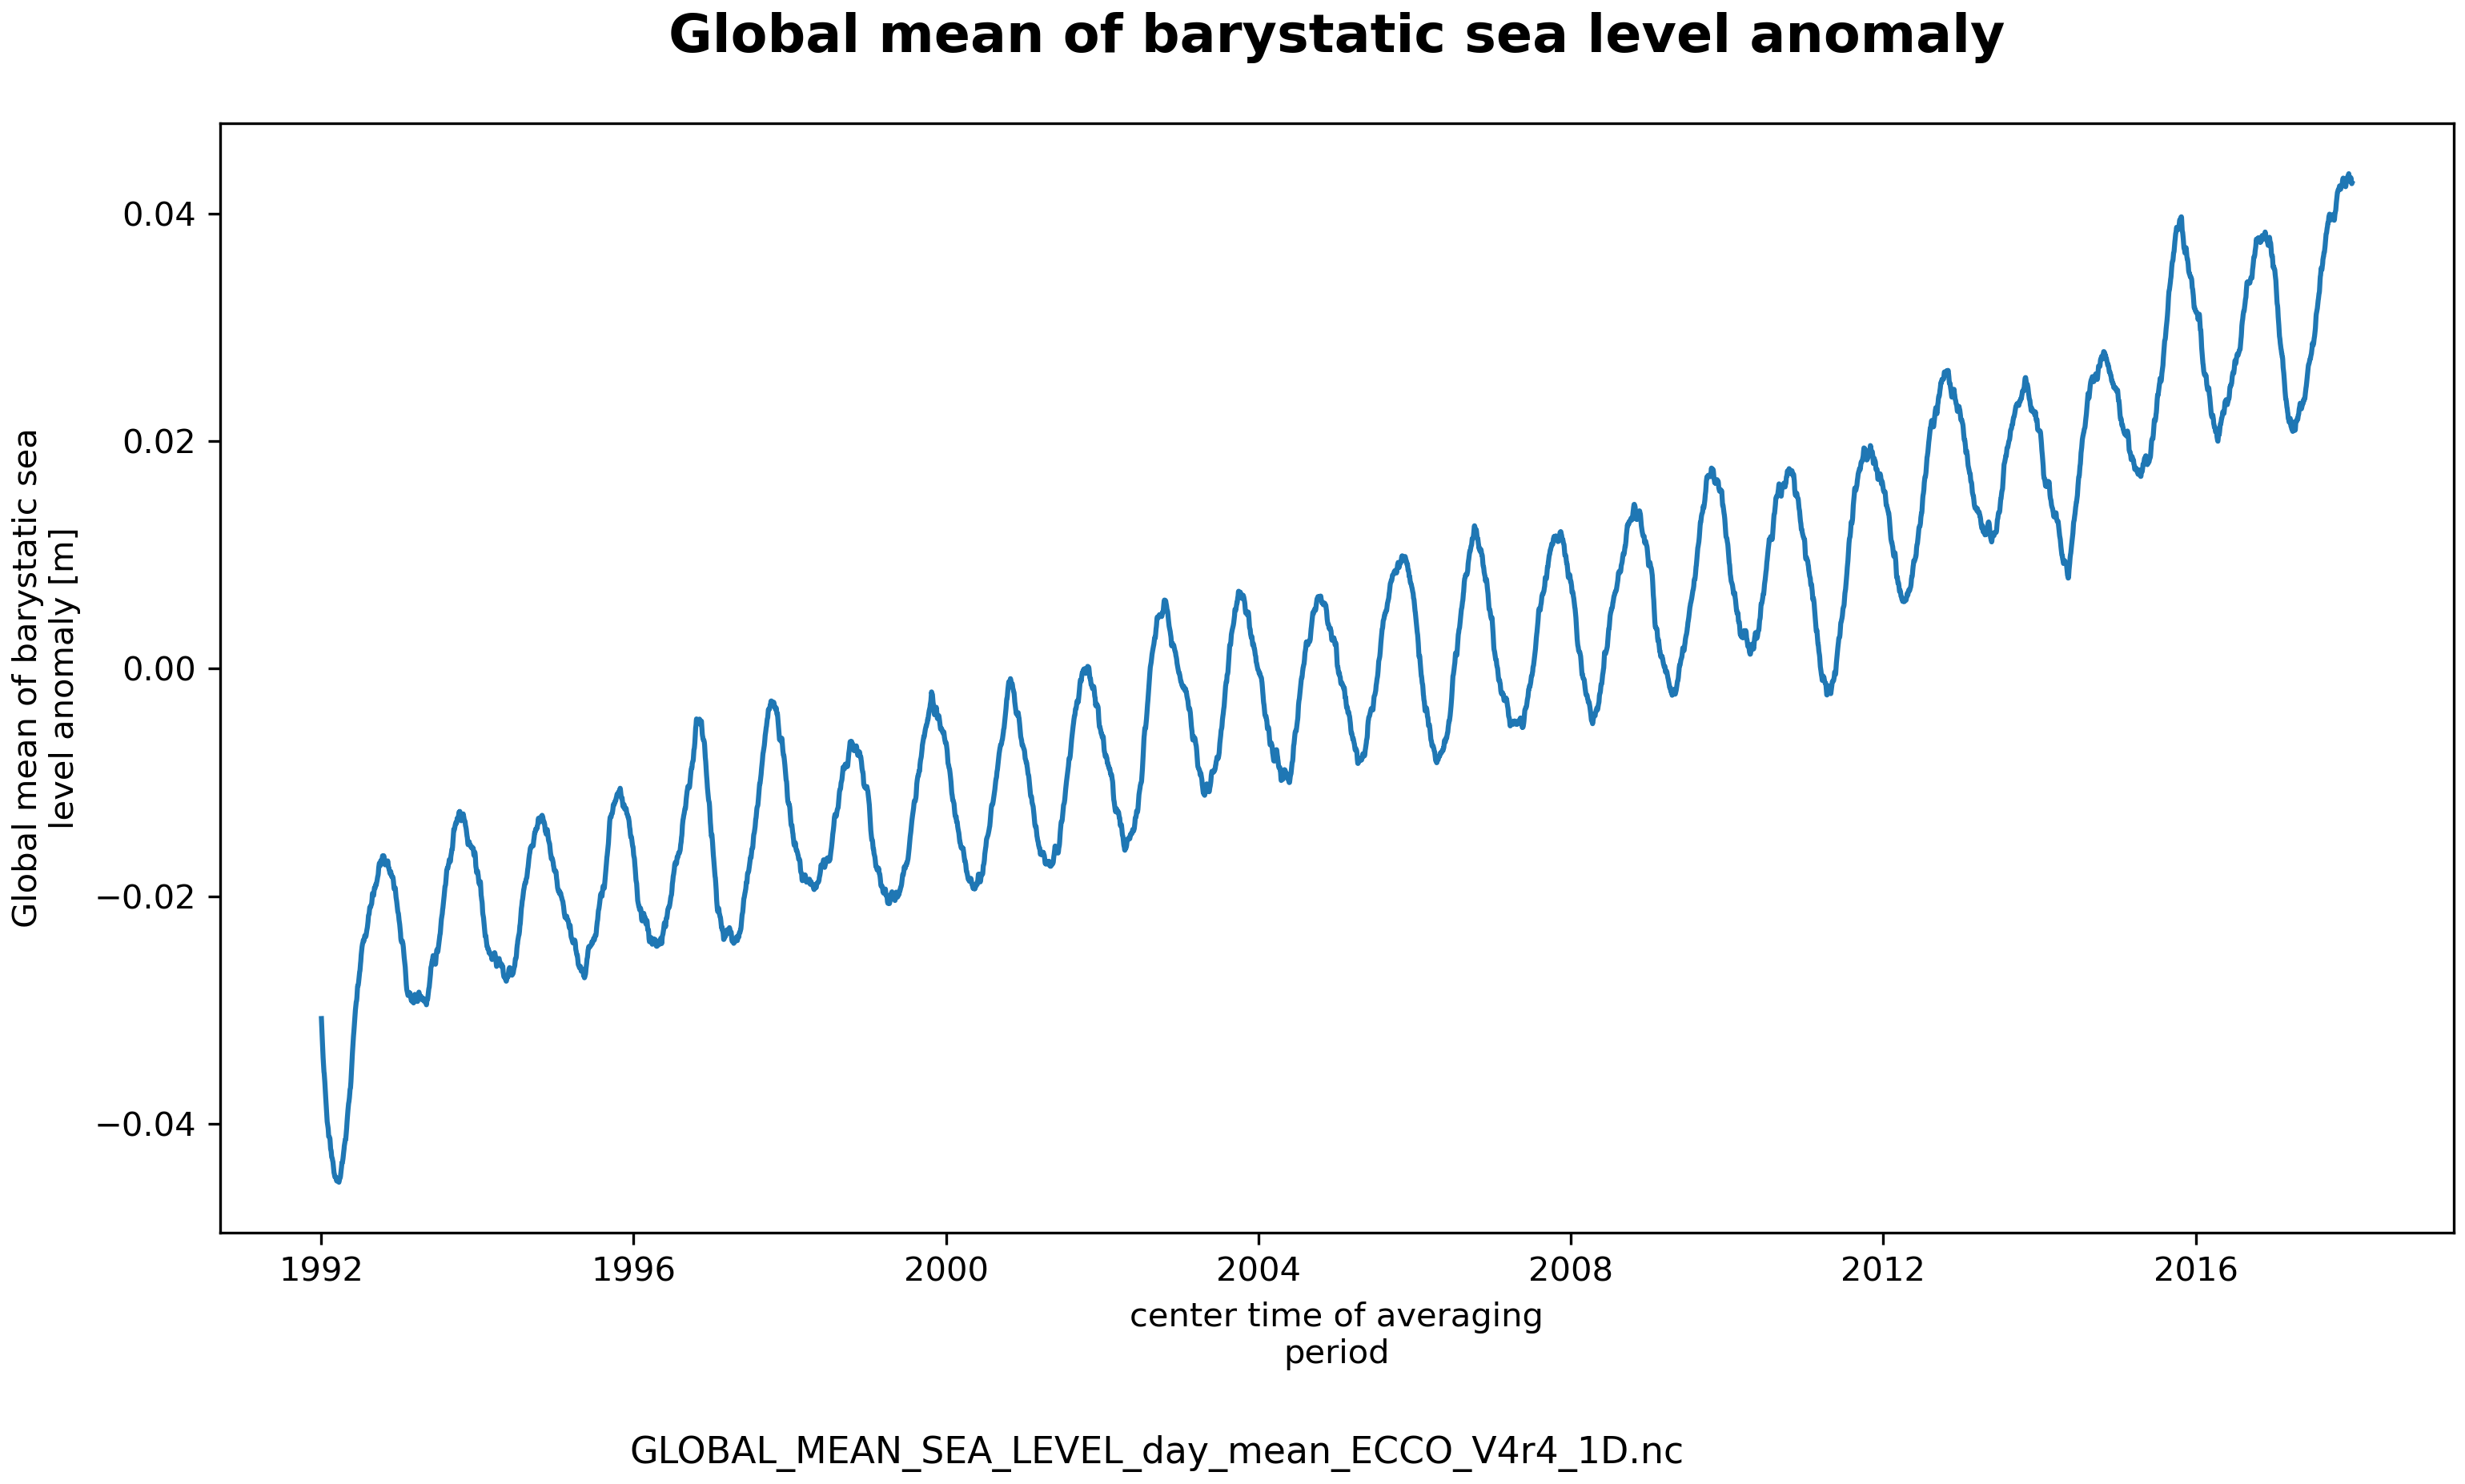
\includegraphics[scale=0.55]{../images/plots/v4r4/oneD_plots/Global_Mean_Sea_Level/global_mean_barystatic_sea_level_anomaly.png}
\caption{Dataset: GLOBAL\_MEAN\_SEA\_LEVEL, Variable: global\_mean\_barystatic\_sea\_level\_anomaly}
\label{tab:table-GLOBAL_MEAN_SEA_LEVEL_global_mean_barystatic_sea_level_anomaly-Plot}
\end{figure}
\newpage
\pagebreak
\subsubsection{1D Variable: global\_mean\_sea\_level\_anomaly}
\begin{longtable}{|m{0.06\textwidth}|m{0.44\textwidth}|m{0.38\textwidth}|m{0.12\textwidth}|}
\caption{Attributes description of the variable 'global\_mean\_sea\_level\_anomaly' from GLOBAL\_MEAN\_SEA\_LEVEL's  dataset.}
\label{tab:table-GLOBAL_MEAN_SEA_LEVEL_global_mean_sea_level_anomaly} \\ 
\hline \endhead \hline \endfoot
\rowcolor{lightgray} \textbf{Storage Type} & \textbf{Variable Name} & \textbf{Description} & \textbf{Unit} \\ \hline
float32 & global\_mean\_sea\_level\_anomaly & Global mean of dynamic ssh & m \\ \hline
\multicolumn{4}{|c|}{\cellcolor{lightgray}{\textbf{Description of the variable in Common Data language (CDL)}}} \\ \hline
\multicolumn{4}{|c|}{\fontfamily{lmtt}\selectfont{\makecell{\parbox{.95\textwidth}{\vspace*{0.25cm} \footnotesize{float32 global\_mean\_sea\_level\_anomaly(time)\\
\hspace*{0.5cm}global\_mean\_sea\_level\_anomaly: \_FillValue = 9.96921e+36\\
\hspace*{0.5cm}global\_mean\_sea\_level\_anomaly: coordinates = time\\
\hspace*{0.5cm}global\_mean\_sea\_level\_anomaly: coverage\_content\_type = modelResult\\
\hspace*{0.5cm}global\_mean\_sea\_level\_anomaly: long\_name = Global mean of dynamic SSH\\
\hspace*{0.5cm}global\_mean\_sea\_level\_anomaly: standard\_name = \\
\hspace*{0.5cm}global\_mean\_sea\_level\_anomaly: units = m\\
\hspace*{0.5cm}global\_mean\_sea\_level\_anomaly: valid\_max = 0.05520557\\
\hspace*{0.5cm}global\_mean\_sea\_level\_anomaly: valid\_min = -0.055836163\\
}}}}} \\ \hline
\rowcolor{lightgray} \multicolumn{4}{|c|}{\textbf{Comments}} \\ \hline
\multicolumn{4}{|p{1\textwidth}|}{\footnotesize{{Global mean of dynamic sea level anomaly, equivalent to global mean sea level change. note: eccov4 uses a volume-conserving boussinesq formulation of the mitgcm with a free-surface boundary condition with real freshwater flux forcing. changes in ocean mass due to evaporation, precipitation, runoff, and sea-ice growth/melt are reflected in model sea level. however, as a consequence of the boussinsq formulation, changes to seawater density due to net buoyancy fluxes (e.g., global mean surface heating/cooling) do not change model sea level anomaly (etan) via seawater expansion/contraction. changes in global ocean density therefore induce a spurious change in model ocean bottom pressure (phibot) via 'virtual mass fluxes'. the 'greatbatch correction' is a time varying, globally-uniform correction to account for changes in global mean density in boussinesq models. this correction is used to calculate dynamic sea surface height (ssh) and ocean bottom pressure (obp). importantly, there is no dynamical significance to the greatbatch correction but it is required to account for steric changes in global sea level. see greatbatch, 1994. j. of geophys. res. oceans, doi.org/10.1029/94jc00847}}} \\ \hline
\end{longtable}

\begin{figure}[H]
\centering
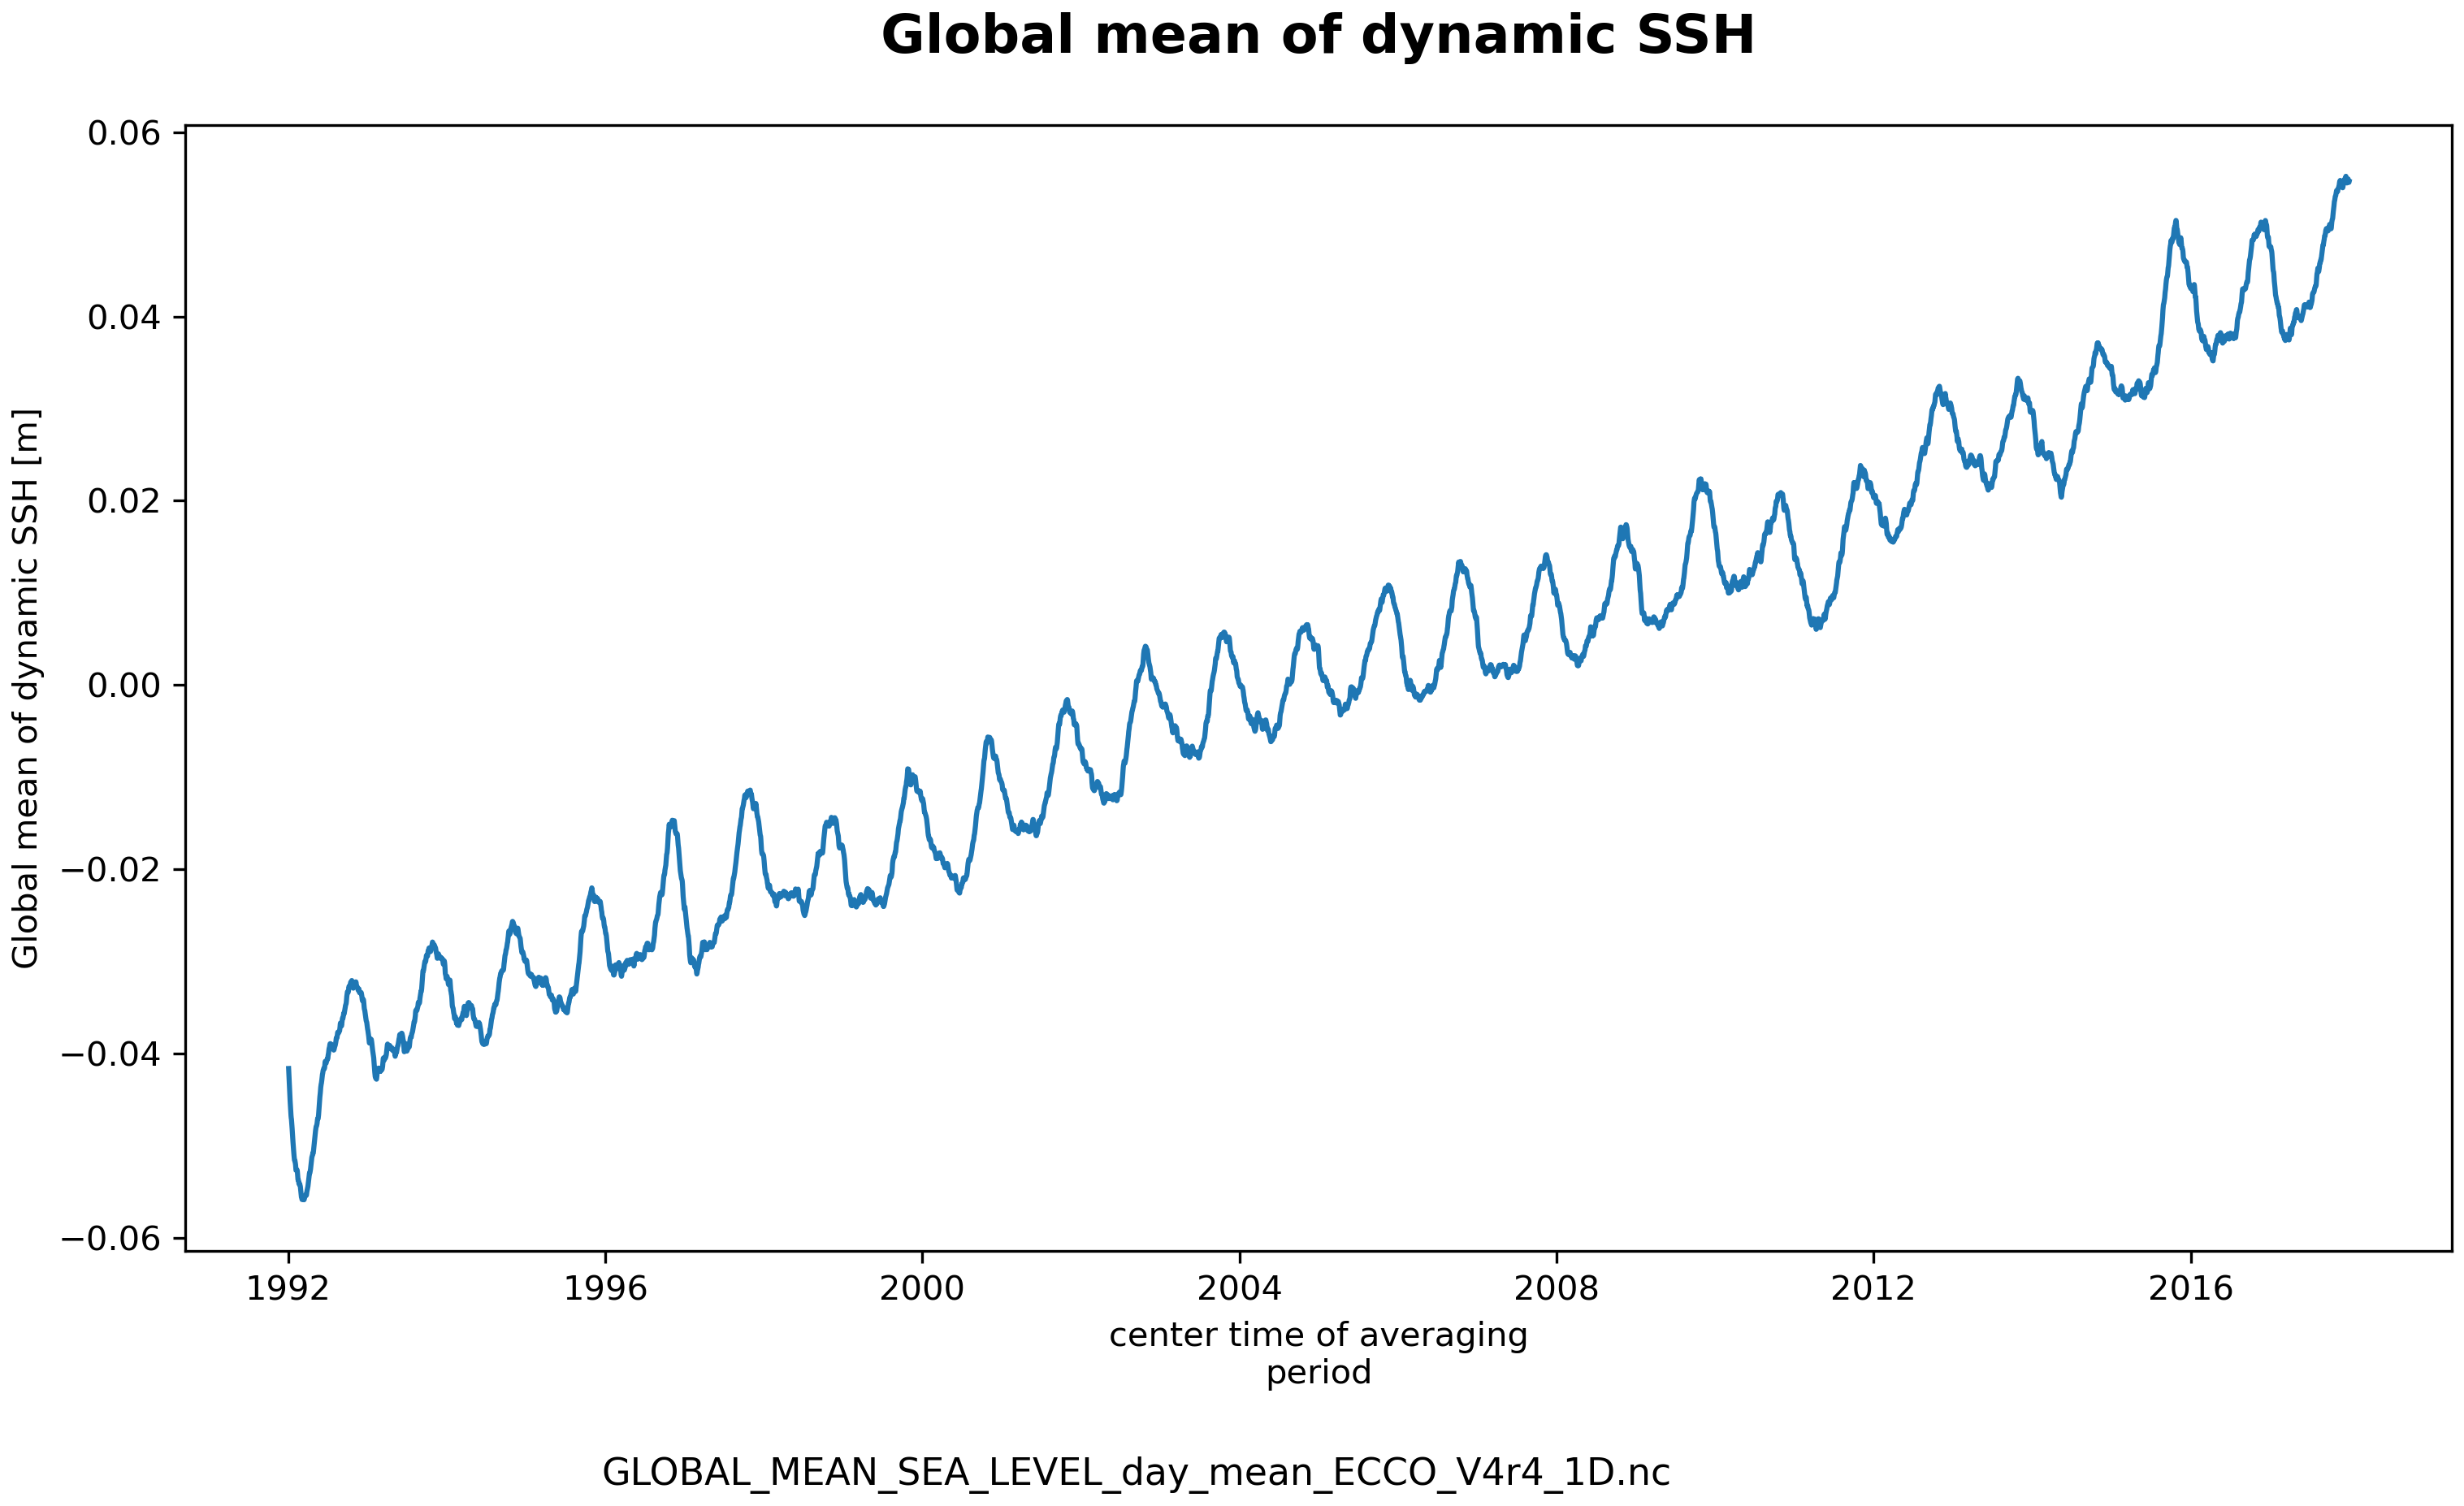
\includegraphics[scale=0.55]{../images/plots/v4r4/oneD_plots/Global_Mean_Sea_Level/global_mean_sea_level_anomaly.png}
\caption{Dataset: GLOBAL\_MEAN\_SEA\_LEVEL, Variable: global\_mean\_sea\_level\_anomaly}
\label{tab:table-GLOBAL_MEAN_SEA_LEVEL_global_mean_sea_level_anomaly-Plot}
\end{figure}
\newpage
\pagebreak
\subsubsection{1D Variable: global\_mean\_sterodynamic\_sea\_level\_anomaly}
\begin{longtable}{|m{0.06\textwidth}|m{0.44\textwidth}|m{0.38\textwidth}|m{0.12\textwidth}|}
\caption{Attributes description of the variable 'global\_mean\_sterodynamic\_sea\_level\_anomaly' from GLOBAL\_MEAN\_SEA\_LEVEL's  dataset.}
\label{tab:table-GLOBAL_MEAN_SEA_LEVEL_global_mean_sterodynamic_sea_level_anomaly} \\ 
\hline \endhead \hline \endfoot
\rowcolor{lightgray} \textbf{Storage Type} & \textbf{Variable Name} & \textbf{Description} & \textbf{Unit} \\ \hline
float64 & global\_mean\_sterodynamic\_sea\_level\_anomaly & Global mean of sterodynamic sea level anomaly & m \\ \hline
\multicolumn{4}{|c|}{\cellcolor{lightgray}{\textbf{Description of the variable in Common Data language (CDL)}}} \\ \hline
\multicolumn{4}{|c|}{\fontfamily{lmtt}\selectfont{\makecell{\parbox{.95\textwidth}{\vspace*{0.25cm} \footnotesize{float64 global\_mean\_sterodynamic\_sea\_level\_anomaly(time)\\
\hspace*{0.5cm}global\_mean\_sterodynamic\_sea\_level\_anomaly: \_FillValue = 9.969209968386869e+36\\
\hspace*{0.5cm}global\_mean\_sterodynamic\_sea\_level\_anomaly: coordinates = time\\
\hspace*{0.5cm}global\_mean\_sterodynamic\_sea\_level\_anomaly: coverage\_content\_type = modelResult\\
\hspace*{0.5cm}global\_mean\_sterodynamic\_sea\_level\_anomaly: long\_name = Global mean of sterodynamic sea level anomaly\\
\hspace*{0.5cm}global\_mean\_sterodynamic\_sea\_level\_anomaly: standard\_name = \\
\hspace*{0.5cm}global\_mean\_sterodynamic\_sea\_level\_anomaly: units = m\\
\hspace*{0.5cm}global\_mean\_sterodynamic\_sea\_level\_anomaly: valid\_max = 0.017642477223663407\\
\hspace*{0.5cm}global\_mean\_sterodynamic\_sea\_level\_anomaly: valid\_min = -0.017658796143049296\\
}}}}} \\ \hline
\rowcolor{lightgray} \multicolumn{4}{|c|}{\textbf{Comments}} \\ \hline
\multicolumn{4}{|p{1\textwidth}|}{\footnotesize{{Steric sea level anomaly associated with seawater expansion/contraction due to density changes. note: eccov4 uses a volume-conserving boussinesq formulation of the mitgcm with a free-surface boundary condition with real freshwater flux forcing. changes in ocean mass due to evaporation, precipitation, runoff, and sea-ice growth/melt are reflected in model sea level. however, as a consequence of the boussinsq formulation, changes to seawater density due to net buoyancy fluxes (e.g., global mean surface heating/cooling) do not change model sea level anomaly (etan) via seawater expansion/contraction. changes in global ocean density therefore induce a spurious change in model ocean bottom pressure (phibot) via 'virtual mass fluxes'. the 'greatbatch correction' is a time varying, globally-uniform correction to account for changes in global mean density in boussinesq models. this correction is used to calculate dynamic sea surface height (ssh) and ocean bottom pressure (obp). importantly, there is no dynamical significance to the greatbatch correction but it is required to account for steric changes in global sea level. see greatbatch, 1994. j. of geophys. res. oceans, doi.org/10.1029/94jc00847}}} \\ \hline
\end{longtable}

\begin{figure}[H]
\centering
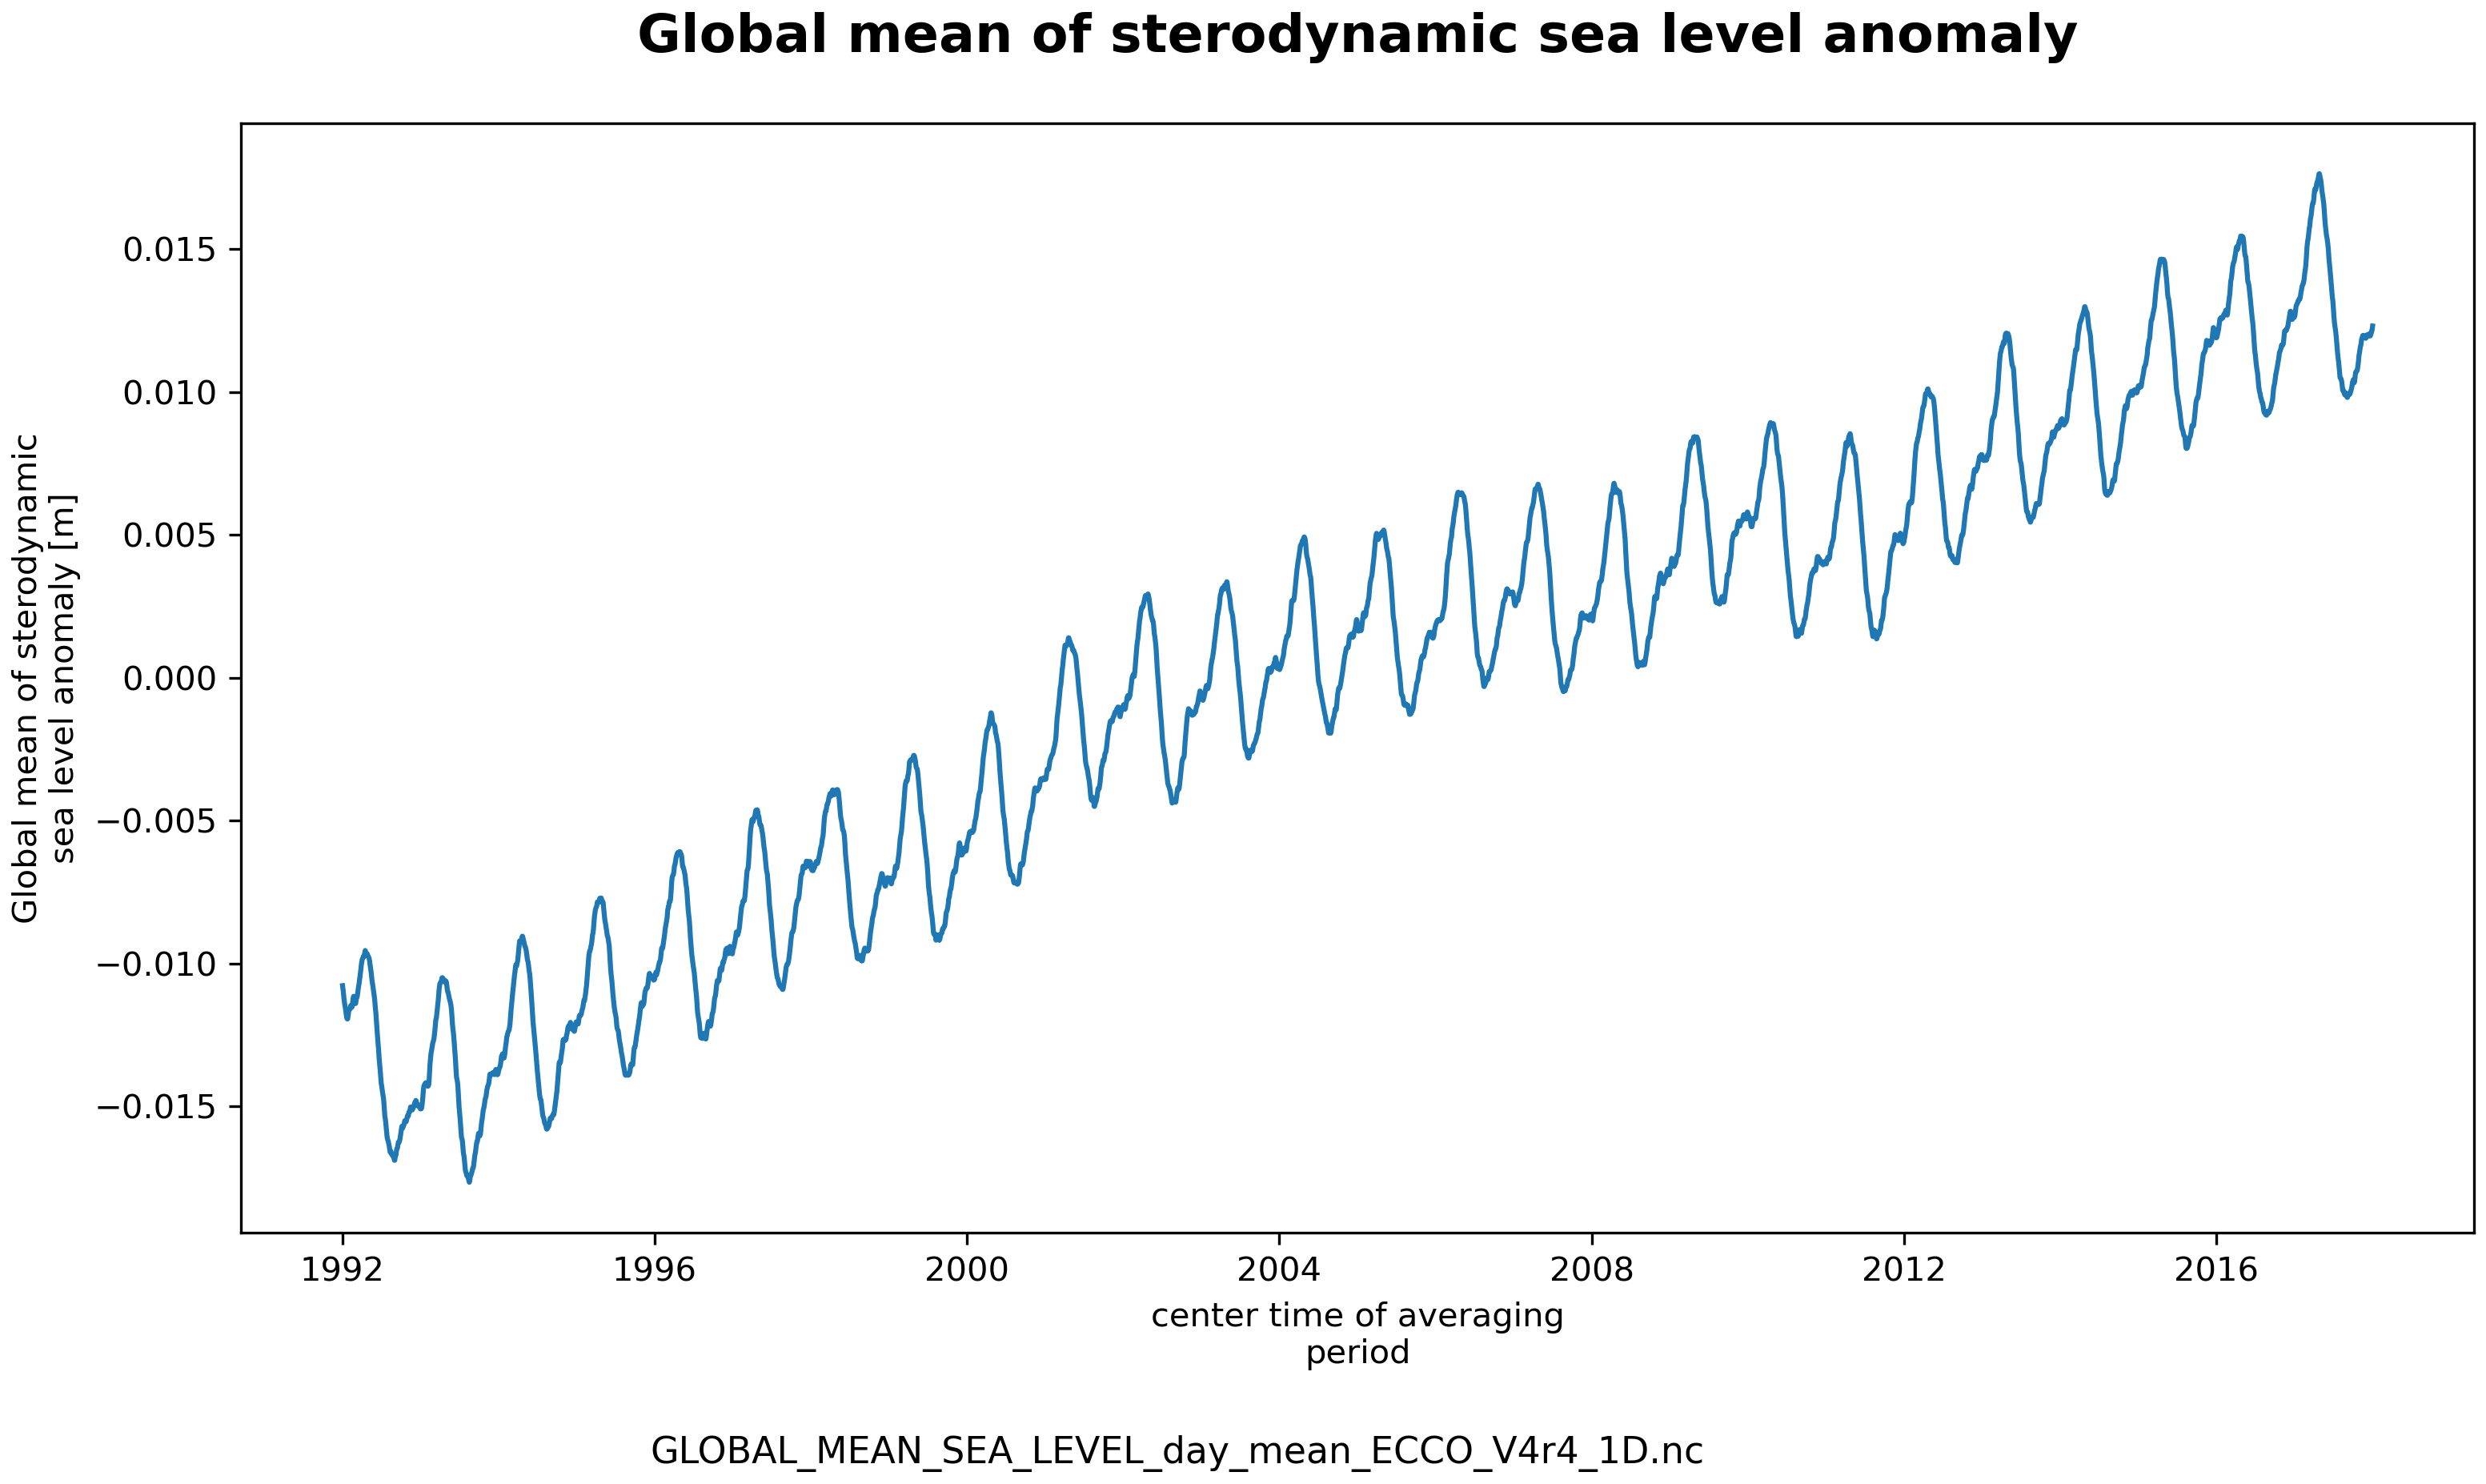
\includegraphics[scale=0.55]{../images/plots/v4r4/oneD_plots/Global_Mean_Sea_Level/global_mean_sterodynamic_sea_level_anomaly.png}
\caption{Dataset: GLOBAL\_MEAN\_SEA\_LEVEL, Variable: global\_mean\_sterodynamic\_sea\_level\_anomaly}
\label{tab:table-GLOBAL_MEAN_SEA_LEVEL_global_mean_sterodynamic_sea_level_anomaly-Plot}
\end{figure}
\newpage
\subsection{1D dataset of SBO\_CORE\_PRODUCTS}
\newp
\subsubsection{Overview}
This dataset provides a 1D field of the core products of the IERS Special Bureau for the Oceans from the ECCO Version 4 Release 4 (V4r4) ocean and sea-ice state estimate. The dataset is provided on instantaneous hourly snapshot aas well as daily-average and monthly-average time resolution. Dataset fields include core products of the IERS Special Bureau for the Oceans (https://euler.jpl.nasa.gov/sbo/sbo\_home.html), including ocean angular momentum (OAM), center of mass (COM) and global ocean mass, calculated using the basic formulation of Gross et al. (2000). Further details on the available fields are provided in Quinn et al. (2019). 
\begin{longtable}{|m{0.15\textwidth}|m{0.64\textwidth}|m{0.12\textwidth}|}
\caption{Coordinates and Variables in the dataset SBO\_CORE\_PRODUCTS}
\label{tab:table-SBO_CORE_PRODUCTS-fields} \\ 
\hline \endhead \hline \endfoot
\rowcolor{lightgray} \multicolumn{1}{|c|}{\textbf{Coordinates}} & \multicolumn{1}{|c|}{\textbf{Description of data coordinates}} &  \multicolumn{1}{|c|}{\textbf{Unit}}\\ \hline
time &Snapshot time &--none--  \\ \hline
\rowcolor{lightgray} \multicolumn{1}{|c|}{\textbf{Variables}} & \multicolumn{1}{|c|}{\textbf{Description of data variables}} &  \multicolumn{1}{|c|}{\textbf{Unit}}\\ \hline
xoamc &X-comp of oceanic angular momentum due to currents &kg m2 s-1  \\ \hline
yoamc &Y-comp of oceanic angular momentum due to currents &kg m2 s-1  \\ \hline
zoamc &Z-comp of oceanic angular momentum due to currents &kg m2 s-1  \\ \hline
xoamp &X-comp of oceanic angular momentum due to pressure &kg m2 s-1  \\ \hline
yoamp &Y-comp of oceanic angular momentum due to pressure &kg m2 s-1  \\ \hline
zoamp &Z-comp of oceanic angular momentum due to pressure &kg m2 s-1  \\ \hline
mass &Ocean mass &kg  \\ \hline
xcom &X-comp of center-of-mass of ocean &m  \\ \hline
ycom &Y-comp of center-of-mass of ocean &m  \\ \hline
zcom &Z-comp of center-of-mass of ocean &m  \\ \hline
sboarea &Surface area of oceans &m2  \\ \hline
xoamc\_si &X-comp of oceanic angular momentum due to sea-ice motion &kg m2 s-1  \\ \hline
yoamc\_si &Y-comp of oceanic angular momentum due to sea-ice motion &kg m2 s-1  \\ \hline
zoamc\_si &Z-comp of oceanic angular momentum due to sea-ice motion &kg m2 s-1  \\ \hline
mass\_si &Sea-ice mass &kg  \\ \hline
xoamp\_fw &X-comp of oceanic angular momentum due to freshwater flux &kg m2 s-1  \\ \hline
yoamp\_fw &Y-comp of oceanic angular momentum due to freshwater flux &kg m2 s-1  \\ \hline
zoamp\_fw &Z-comp of oceanic angular momentum due to freshwater flux &kg m2 s-1  \\ \hline
mass\_fw &Mass due to freshwater flux &kg  \\ \hline
xcom\_fw &X-comp of center-of-mass of freshwater flux &m  \\ \hline
ycom\_fw &Y-comp of center-of-mass of freshwater flux &m  \\ \hline
zcom\_fw &Z-comp of center-of-mass of freshater flux &m  \\ \hline
mass\_gc &Mass due to the greatbatch correction &kg  \\ \hline
xoamp\_dsl &X-comp of oceanic angular momentum due to pressure based on dynamic (ib-corrected) sea level &kg m2 s-1  \\ \hline
yoamp\_dsl &Y-comp of oceanic angular momentum due to pressure based on dynamic (ib-corrected) sea level &kg m2 s-1  \\ \hline
zoamp\_dsl &Z-comp of oceanic angular momentum due to pressure based on dynamic (ib-corrected) sea level &kg m2 s-1  \\ \hline
\end{longtable}

\newp
\pagebreak
\subsubsection{1D Variable: mass}
\begin{longtable}{|m{0.06\textwidth}|m{0.3\textwidth}|m{0.45\textwidth}|m{0.12\textwidth}|}
\caption{Attributes description of the variable 'mass' from SBO\_CORE\_PRODUCTS's  dataset.}
\label{tab:table-SBO_CORE_PRODUCTS_mass} \\ 
\hline \endhead \hline \endfoot
\rowcolor{lightgray} \textbf{Storage Type} & \textbf{Variable Name} & \textbf{Description} & \textbf{Unit} \\ \hline
float64 & mass & Ocean mass & kg \\ \hline
\multicolumn{4}{|c|}{\cellcolor{lightgray}{\textbf{Description of the variable in Common Data language (CDL)}}} \\ \hline
\multicolumn{4}{|c|}{\fontfamily{lmtt}\selectfont{\makecell{\parbox{.95\textwidth}{\vspace*{0.25cm} \footnotesize{float64 mass(time)\\
\hspace*{0.5cm}mass: \_FillValue = 9.969209968386869e+36\\
\hspace*{0.5cm}mass: coordinates = time\\
\hspace*{0.5cm}mass: coverage\_content\_type = modelResult\\
\hspace*{0.5cm}mass: long\_name = ocean\hspace*{0.5cm} mass\\
\hspace*{0.5cm}mass: units = kg\\
\hspace*{0.5cm}mass: valid\_max = 1.3737832079900274e+21\\
\hspace*{0.5cm}mass: valid\_min = 1.3737507447512265e+21\\
}}}}} \\ \hline
\rowcolor{lightgray} \multicolumn{4}{|c|}{\textbf{Comments}} \\ \hline
\multicolumn{4}{|p{1\textwidth}|}{\footnotesize{{N/a}}} \\ \hline
\end{longtable}

\begin{figure}[H]
\centering
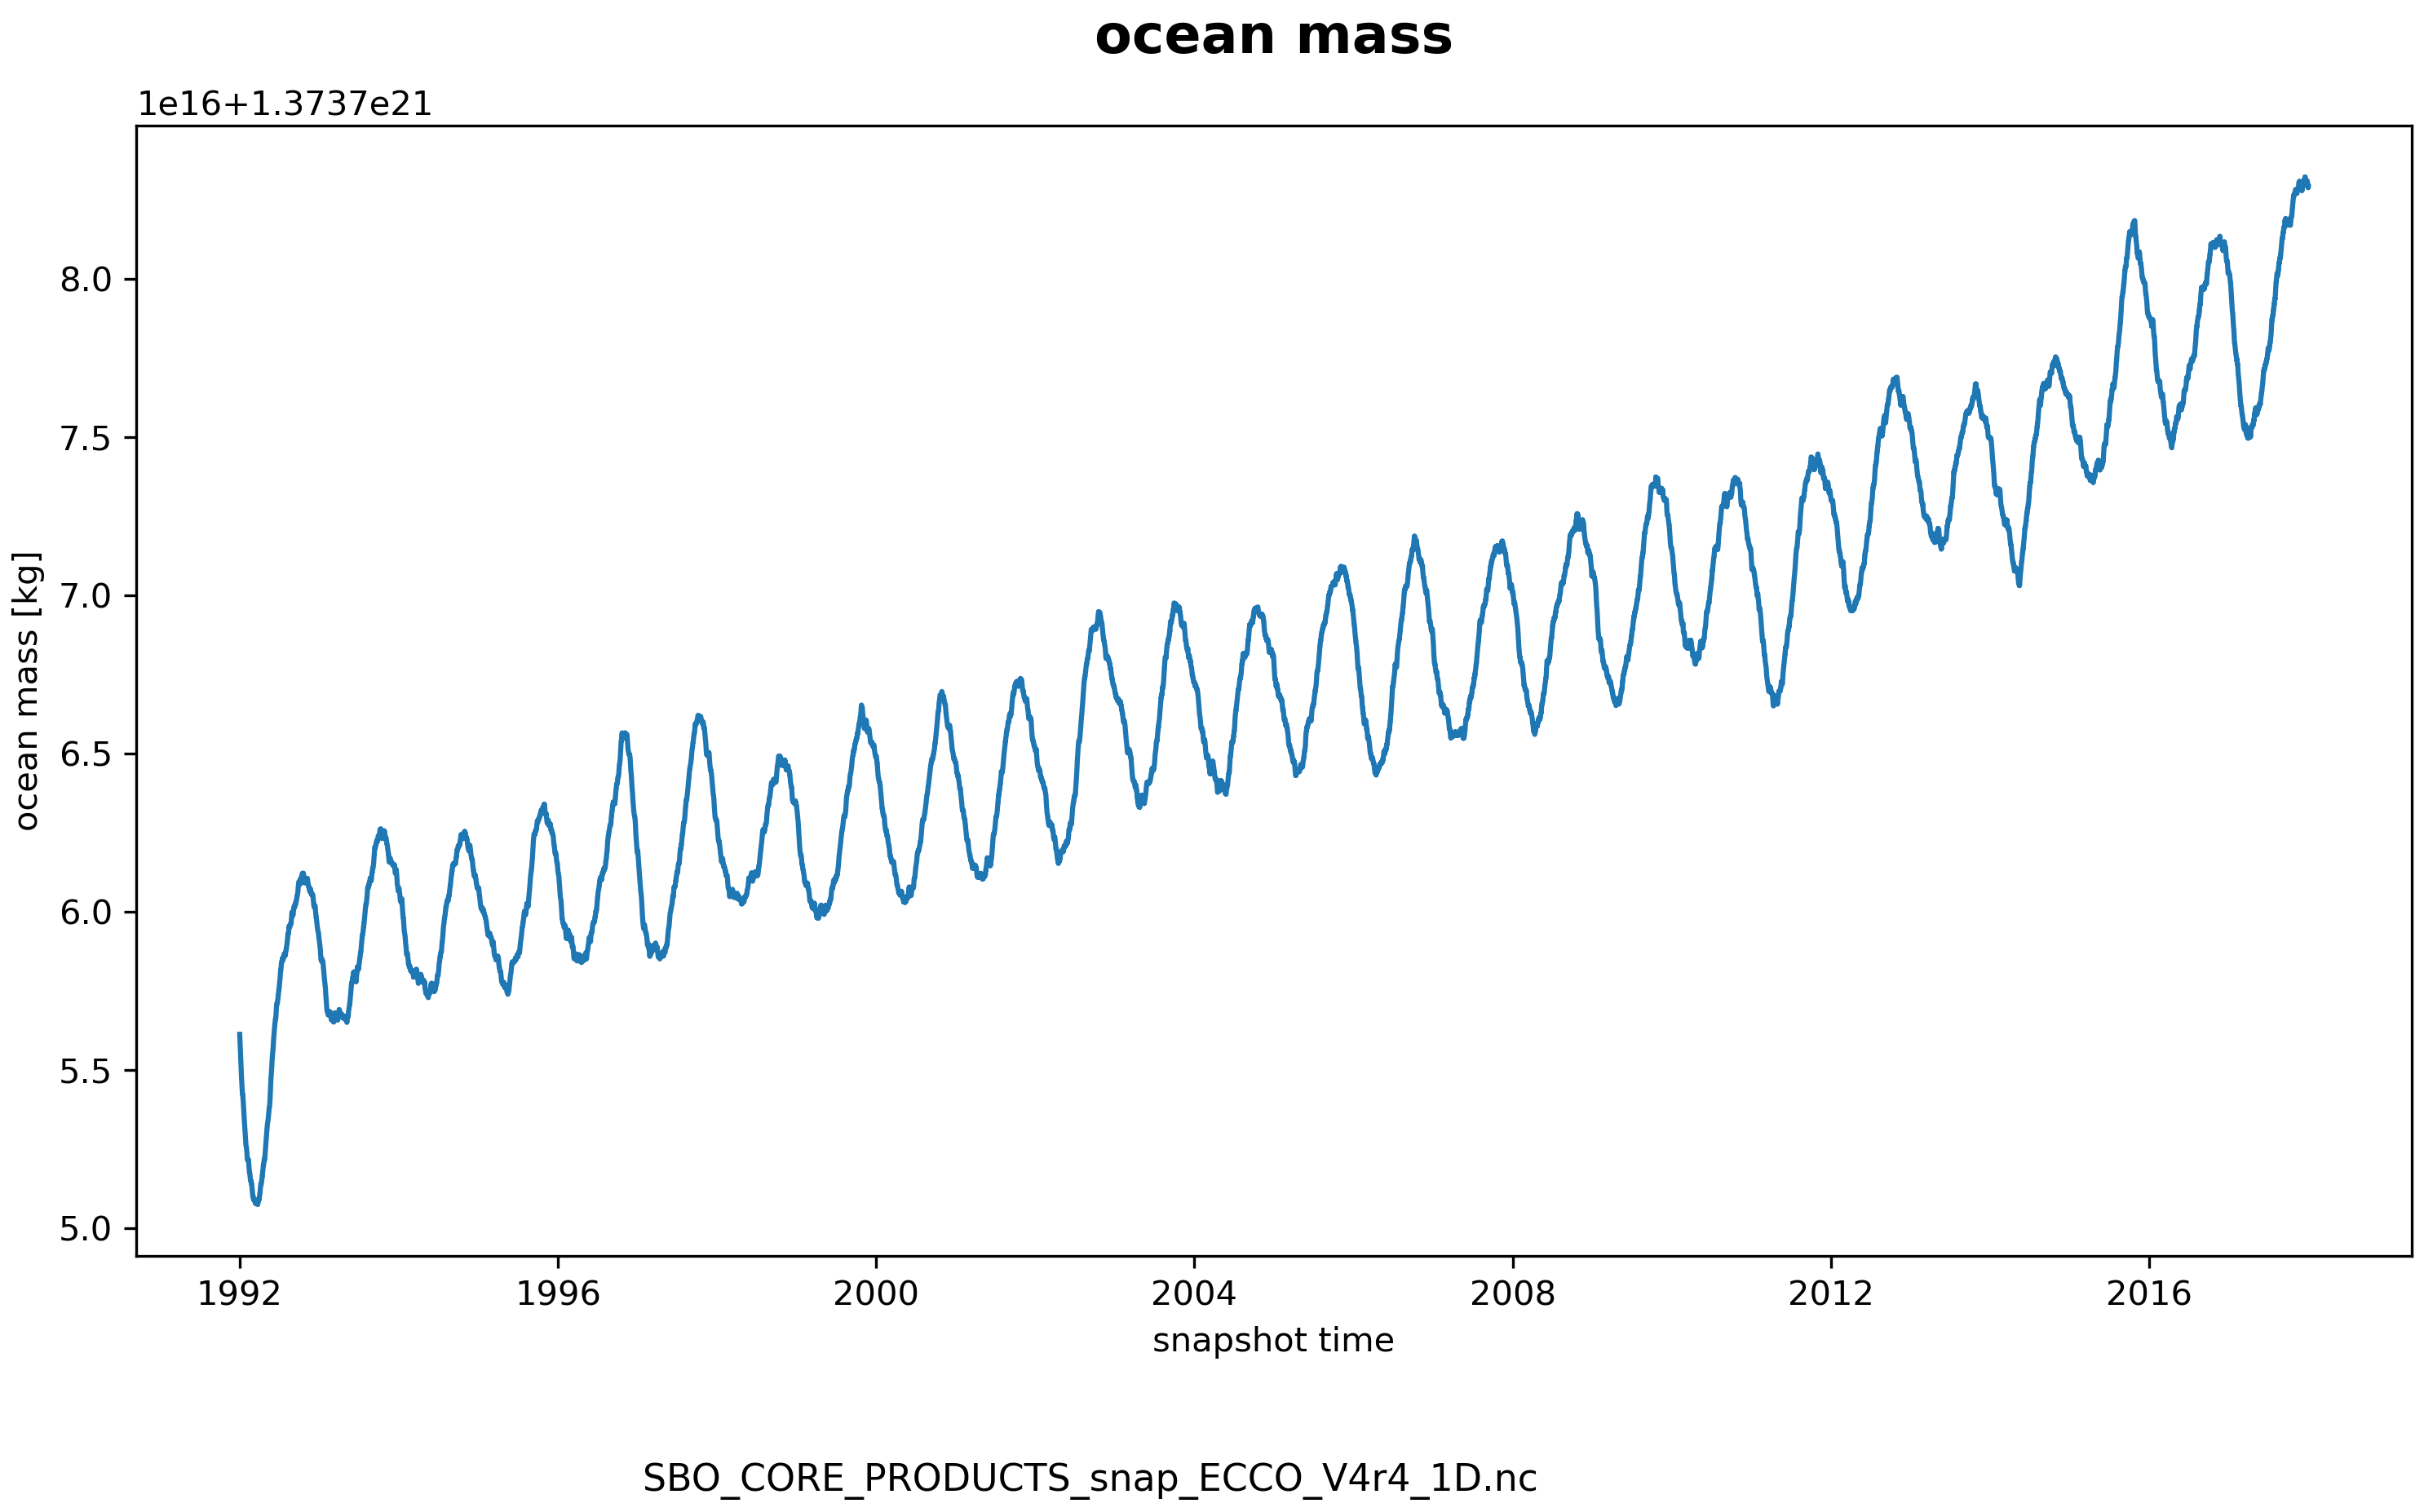
\includegraphics[scale=0.55]{../images/plots/v4r4/oneD_plots/SBO_Core_Products/mass.png}
\caption{Dataset: SBO\_CORE\_PRODUCTS, Variable: mass}
\label{tab:table-SBO_CORE_PRODUCTS_mass-Plot}
\end{figure}
\newpage
\pagebreak
\subsubsection{1D Variable: mass\_fw}
\begin{longtable}{|m{0.06\textwidth}|m{0.3\textwidth}|m{0.45\textwidth}|m{0.12\textwidth}|}
\caption{Attributes description of the variable 'mass\_fw' from SBO\_CORE\_PRODUCTS's  dataset.}
\label{tab:table-SBO_CORE_PRODUCTS_mass_fw} \\ 
\hline \endhead \hline \endfoot
\rowcolor{lightgray} \textbf{Storage Type} & \textbf{Variable Name} & \textbf{Description} & \textbf{Unit} \\ \hline
float64 & mass\_fw & Mass due to freshwater flux & kg \\ \hline
\multicolumn{4}{|c|}{\cellcolor{lightgray}{\textbf{Description of the variable in Common Data language (CDL)}}} \\ \hline
\multicolumn{4}{|c|}{\fontfamily{lmtt}\selectfont{\makecell{\parbox{.95\textwidth}{\vspace*{0.25cm} \footnotesize{float64 mass\_fw(time)\\
\hspace*{0.5cm}mass\_fw: \_FillValue = 9.969209968386869e+36\\
\hspace*{0.5cm}mass\_fw: coordinates = time\\
\hspace*{0.5cm}mass\_fw: coverage\_content\_type = modelResult\\
\hspace*{0.5cm}mass\_fw: long\_name = mass due to freshwater flux\\
\hspace*{0.5cm}mass\_fw: units = kg\\
\hspace*{0.5cm}mass\_fw: valid\_max = 7.0392619494226936e+16\\
\hspace*{0.5cm}mass\_fw: valid\_min = 3.7929380693921944e+16\\
}}}}} \\ \hline
\rowcolor{lightgray} \multicolumn{4}{|c|}{\textbf{Comments}} \\ \hline
\multicolumn{4}{|p{1\textwidth}|}{\footnotesize{{N/a}}} \\ \hline
\end{longtable}

\begin{figure}[H]
\centering
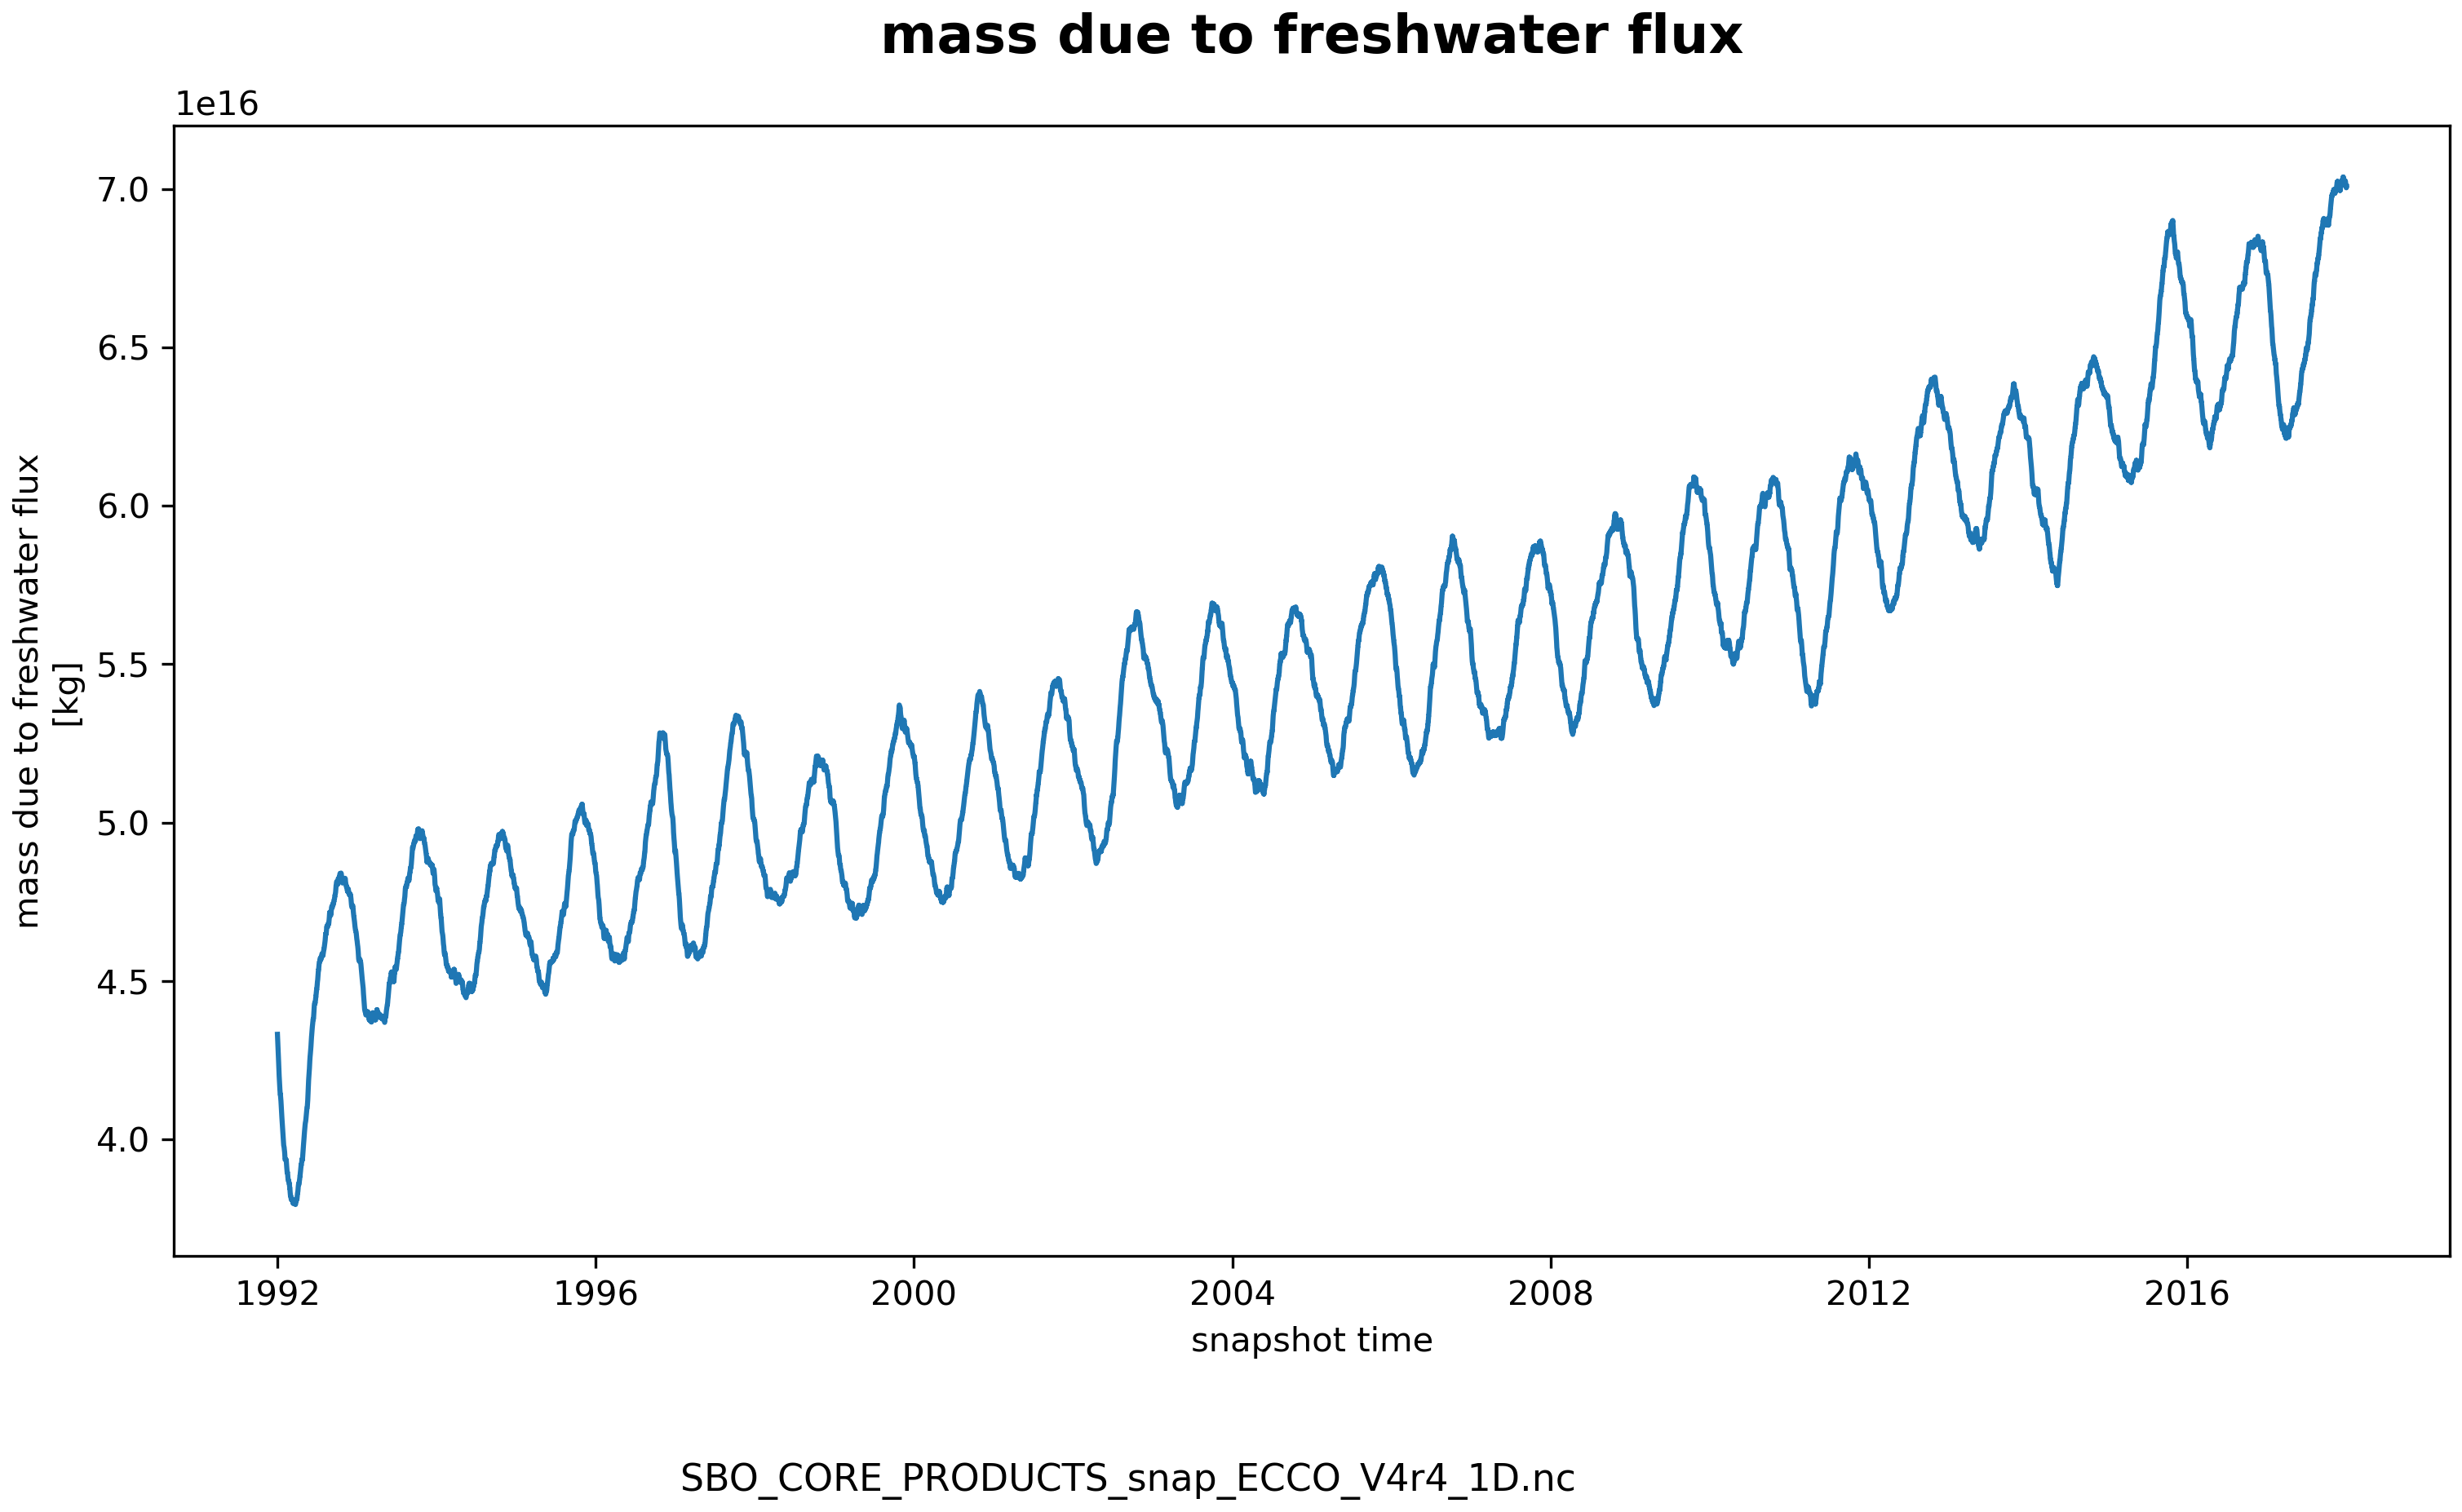
\includegraphics[scale=0.55]{../images/plots/v4r4/oneD_plots/SBO_Core_Products/mass_fw.png}
\caption{Dataset: SBO\_CORE\_PRODUCTS, Variable: mass\_fw}
\label{tab:table-SBO_CORE_PRODUCTS_mass_fw-Plot}
\end{figure}
\newpage
\pagebreak
\subsubsection{1D Variable: mass\_gc}
\begin{longtable}{|m{0.06\textwidth}|m{0.3\textwidth}|m{0.45\textwidth}|m{0.12\textwidth}|}
\caption{Attributes description of the variable 'mass\_gc' from SBO\_CORE\_PRODUCTS's  dataset.}
\label{tab:table-SBO_CORE_PRODUCTS_mass_gc} \\ 
\hline \endhead \hline \endfoot
\rowcolor{lightgray} \textbf{Storage Type} & \textbf{Variable Name} & \textbf{Description} & \textbf{Unit} \\ \hline
float64 & mass\_gc & Mass due to the greatbatch correction & kg \\ \hline
\multicolumn{4}{|c|}{\cellcolor{lightgray}{\textbf{Description of the variable in Common Data language (CDL)}}} \\ \hline
\multicolumn{4}{|c|}{\fontfamily{lmtt}\selectfont{\makecell{\parbox{.95\textwidth}{\vspace*{0.25cm} \footnotesize{float64 mass\_gc(time)\\
\hspace*{0.5cm}mass\_gc: \_FillValue = 9.969209968386869e+36\\
\hspace*{0.5cm}mass\_gc: coordinates = time\\
\hspace*{0.5cm}mass\_gc: coverage\_content\_type = modelResult\\
\hspace*{0.5cm}mass\_gc: long\_name = mass due to the Greatbatch correction\\
\hspace*{0.5cm}mass\_gc: units = kg\\
\hspace*{0.5cm}mass\_gc: valid\_max = -1.1388436906537843e+19\\
\hspace*{0.5cm}mass\_gc: valid\_min = -1.140148294309558e+19\\
}}}}} \\ \hline
\rowcolor{lightgray} \multicolumn{4}{|c|}{\textbf{Comments}} \\ \hline
\multicolumn{4}{|p{1\textwidth}|}{\footnotesize{{N/a}}} \\ \hline
\end{longtable}

\begin{figure}[H]
\centering
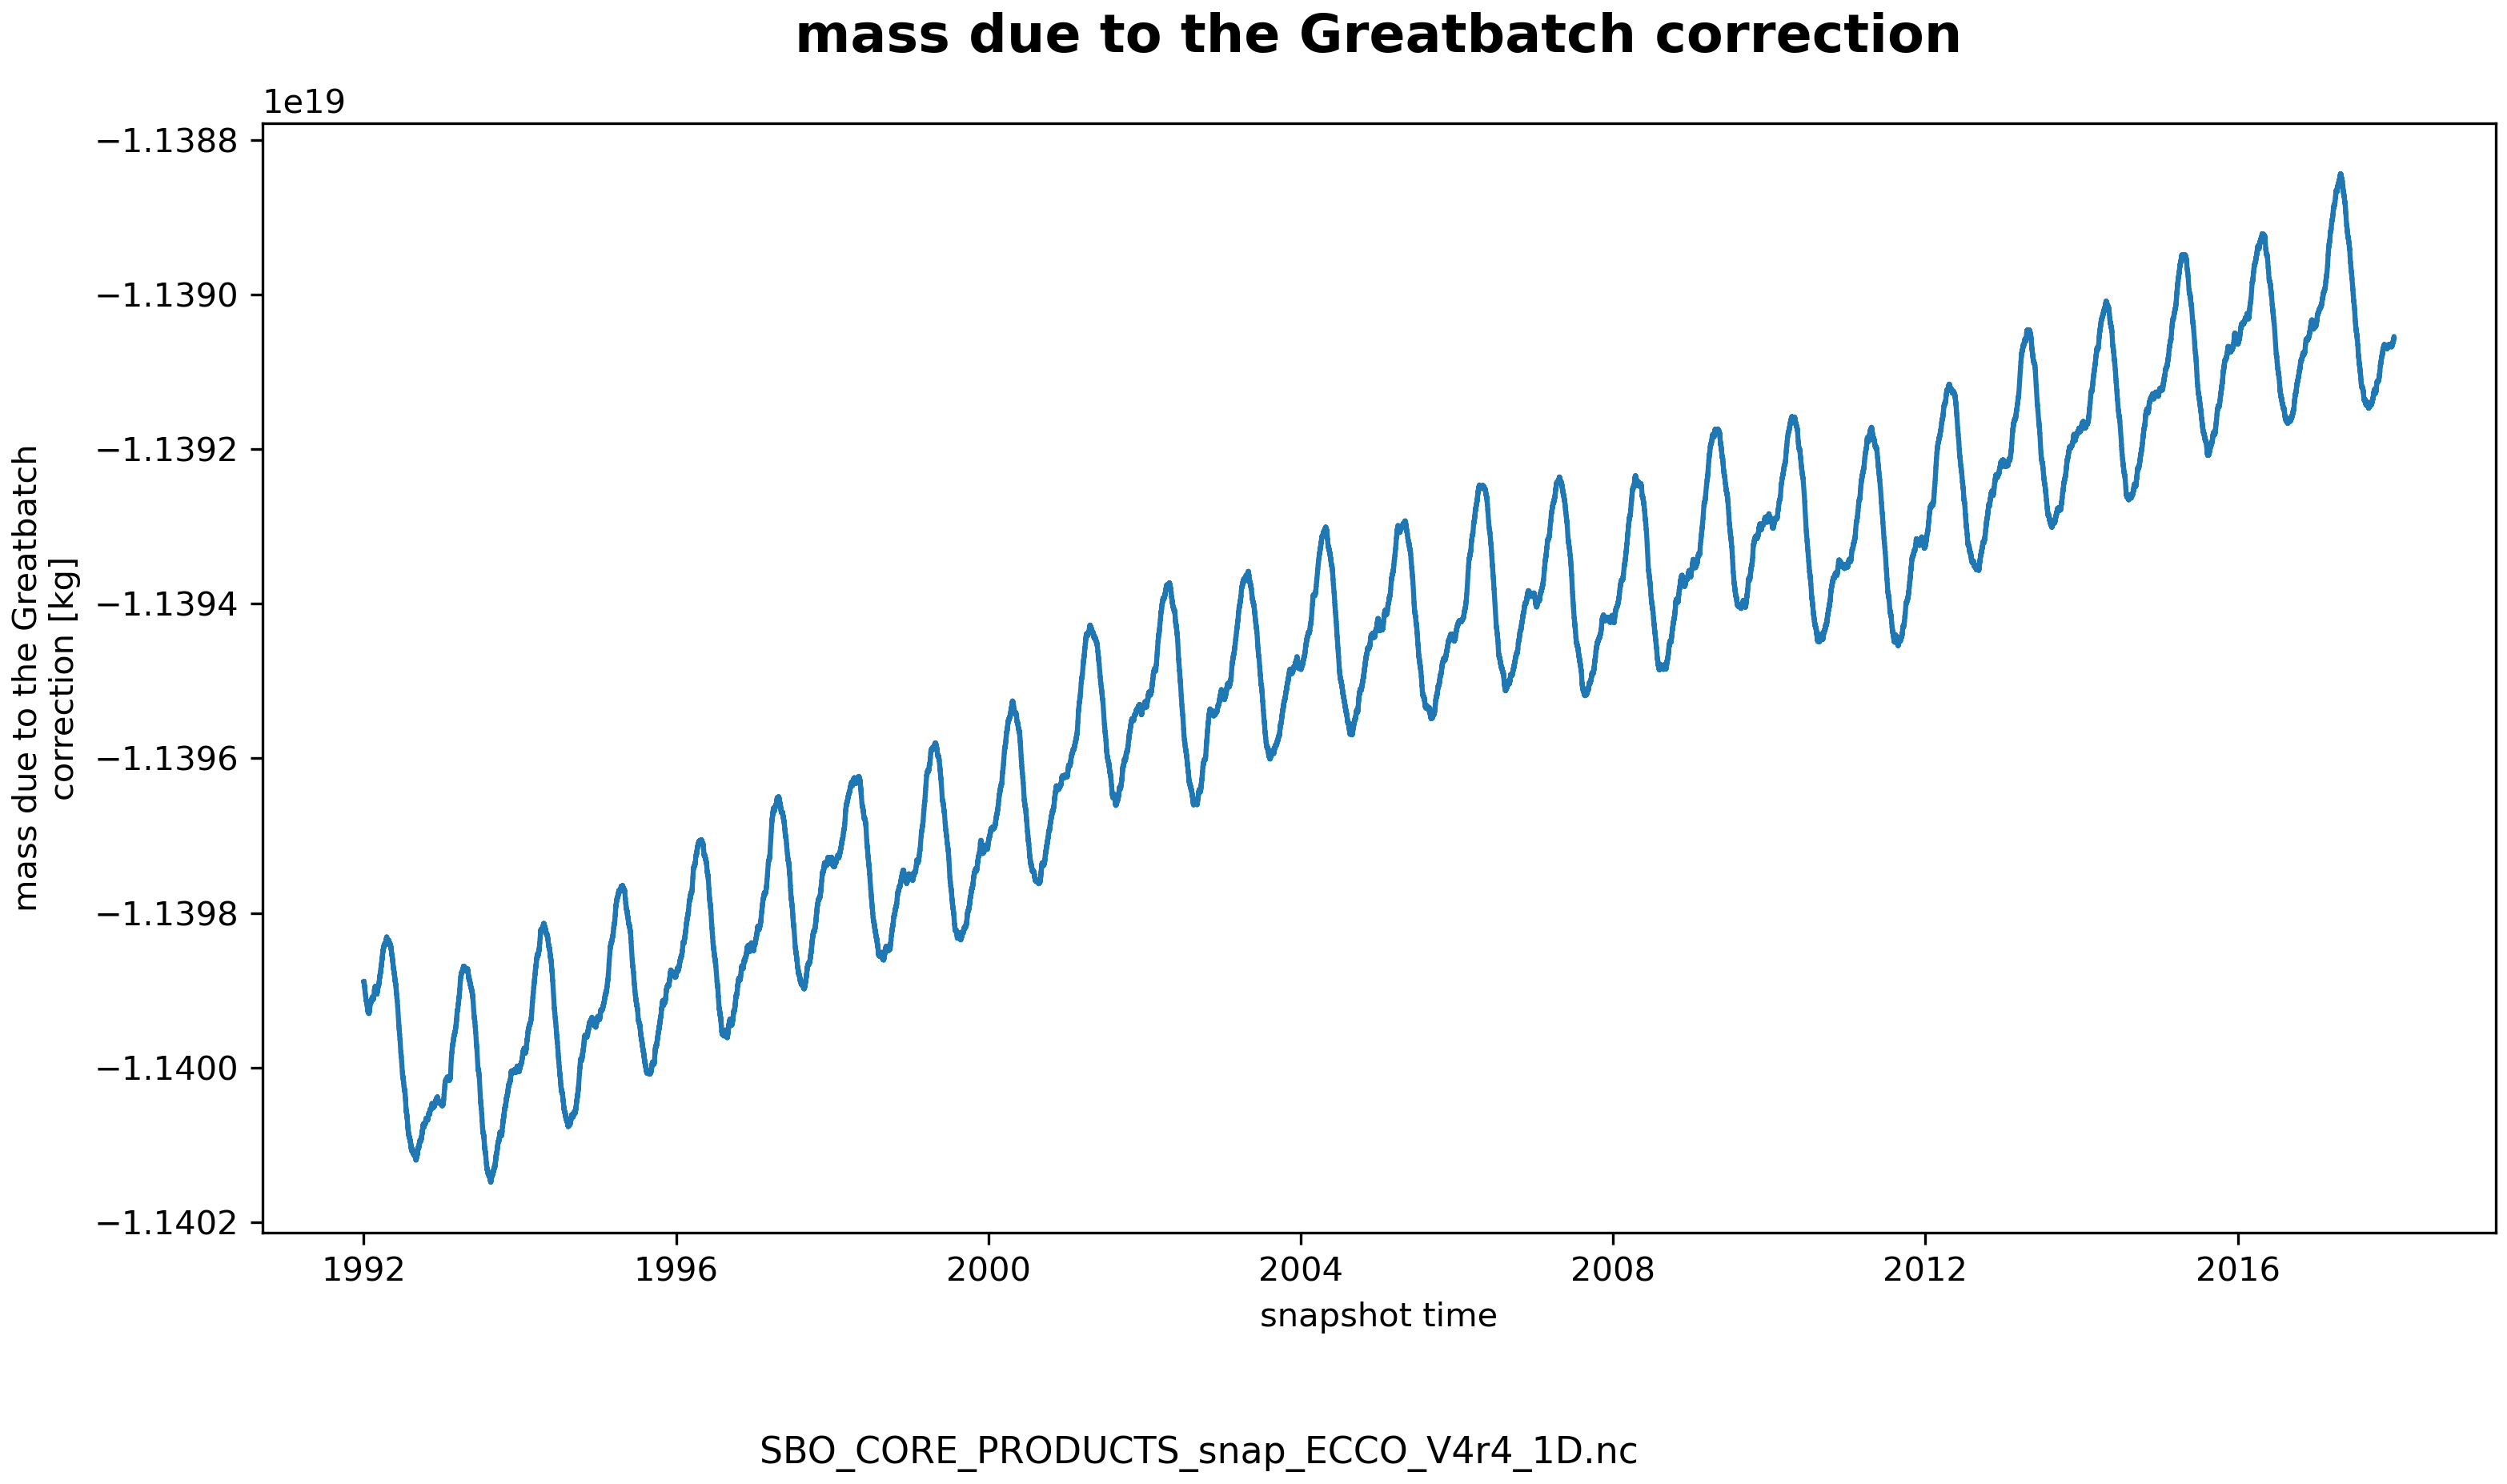
\includegraphics[scale=0.55]{../images/plots/v4r4/oneD_plots/SBO_Core_Products/mass_gc.png}
\caption{Dataset: SBO\_CORE\_PRODUCTS, Variable: mass\_gc}
\label{tab:table-SBO_CORE_PRODUCTS_mass_gc-Plot}
\end{figure}
\newpage
\pagebreak
\subsubsection{1D Variable: mass\_si}
\begin{longtable}{|m{0.06\textwidth}|m{0.3\textwidth}|m{0.45\textwidth}|m{0.12\textwidth}|}
\caption{Attributes description of the variable 'mass\_si' from SBO\_CORE\_PRODUCTS's  dataset.}
\label{tab:table-SBO_CORE_PRODUCTS_mass_si} \\ 
\hline \endhead \hline \endfoot
\rowcolor{lightgray} \textbf{Storage Type} & \textbf{Variable Name} & \textbf{Description} & \textbf{Unit} \\ \hline
float64 & mass\_si & Sea-ice mass & kg \\ \hline
\multicolumn{4}{|c|}{\cellcolor{lightgray}{\textbf{Description of the variable in Common Data language (CDL)}}} \\ \hline
\multicolumn{4}{|c|}{\fontfamily{lmtt}\selectfont{\makecell{\parbox{.95\textwidth}{\vspace*{0.25cm} \footnotesize{float64 mass\_si(time)\\
\hspace*{0.5cm}mass\_si: \_FillValue = 9.969209968386869e+36\\
\hspace*{0.5cm}mass\_si: coordinates = time\\
\hspace*{0.5cm}mass\_si: coverage\_content\_type = modelResult\\
\hspace*{0.5cm}mass\_si: long\_name = sea-ice mass\\
\hspace*{0.5cm}mass\_si: units = kg\\
\hspace*{0.5cm}mass\_si: valid\_max = 3.372421224523182e+16\\
\hspace*{0.5cm}mass\_si: valid\_min = 1.5801085624300974e+16\\
}}}}} \\ \hline
\rowcolor{lightgray} \multicolumn{4}{|c|}{\textbf{Comments}} \\ \hline
\multicolumn{4}{|p{1\textwidth}|}{\footnotesize{{N/a}}} \\ \hline
\end{longtable}

\begin{figure}[H]
\centering
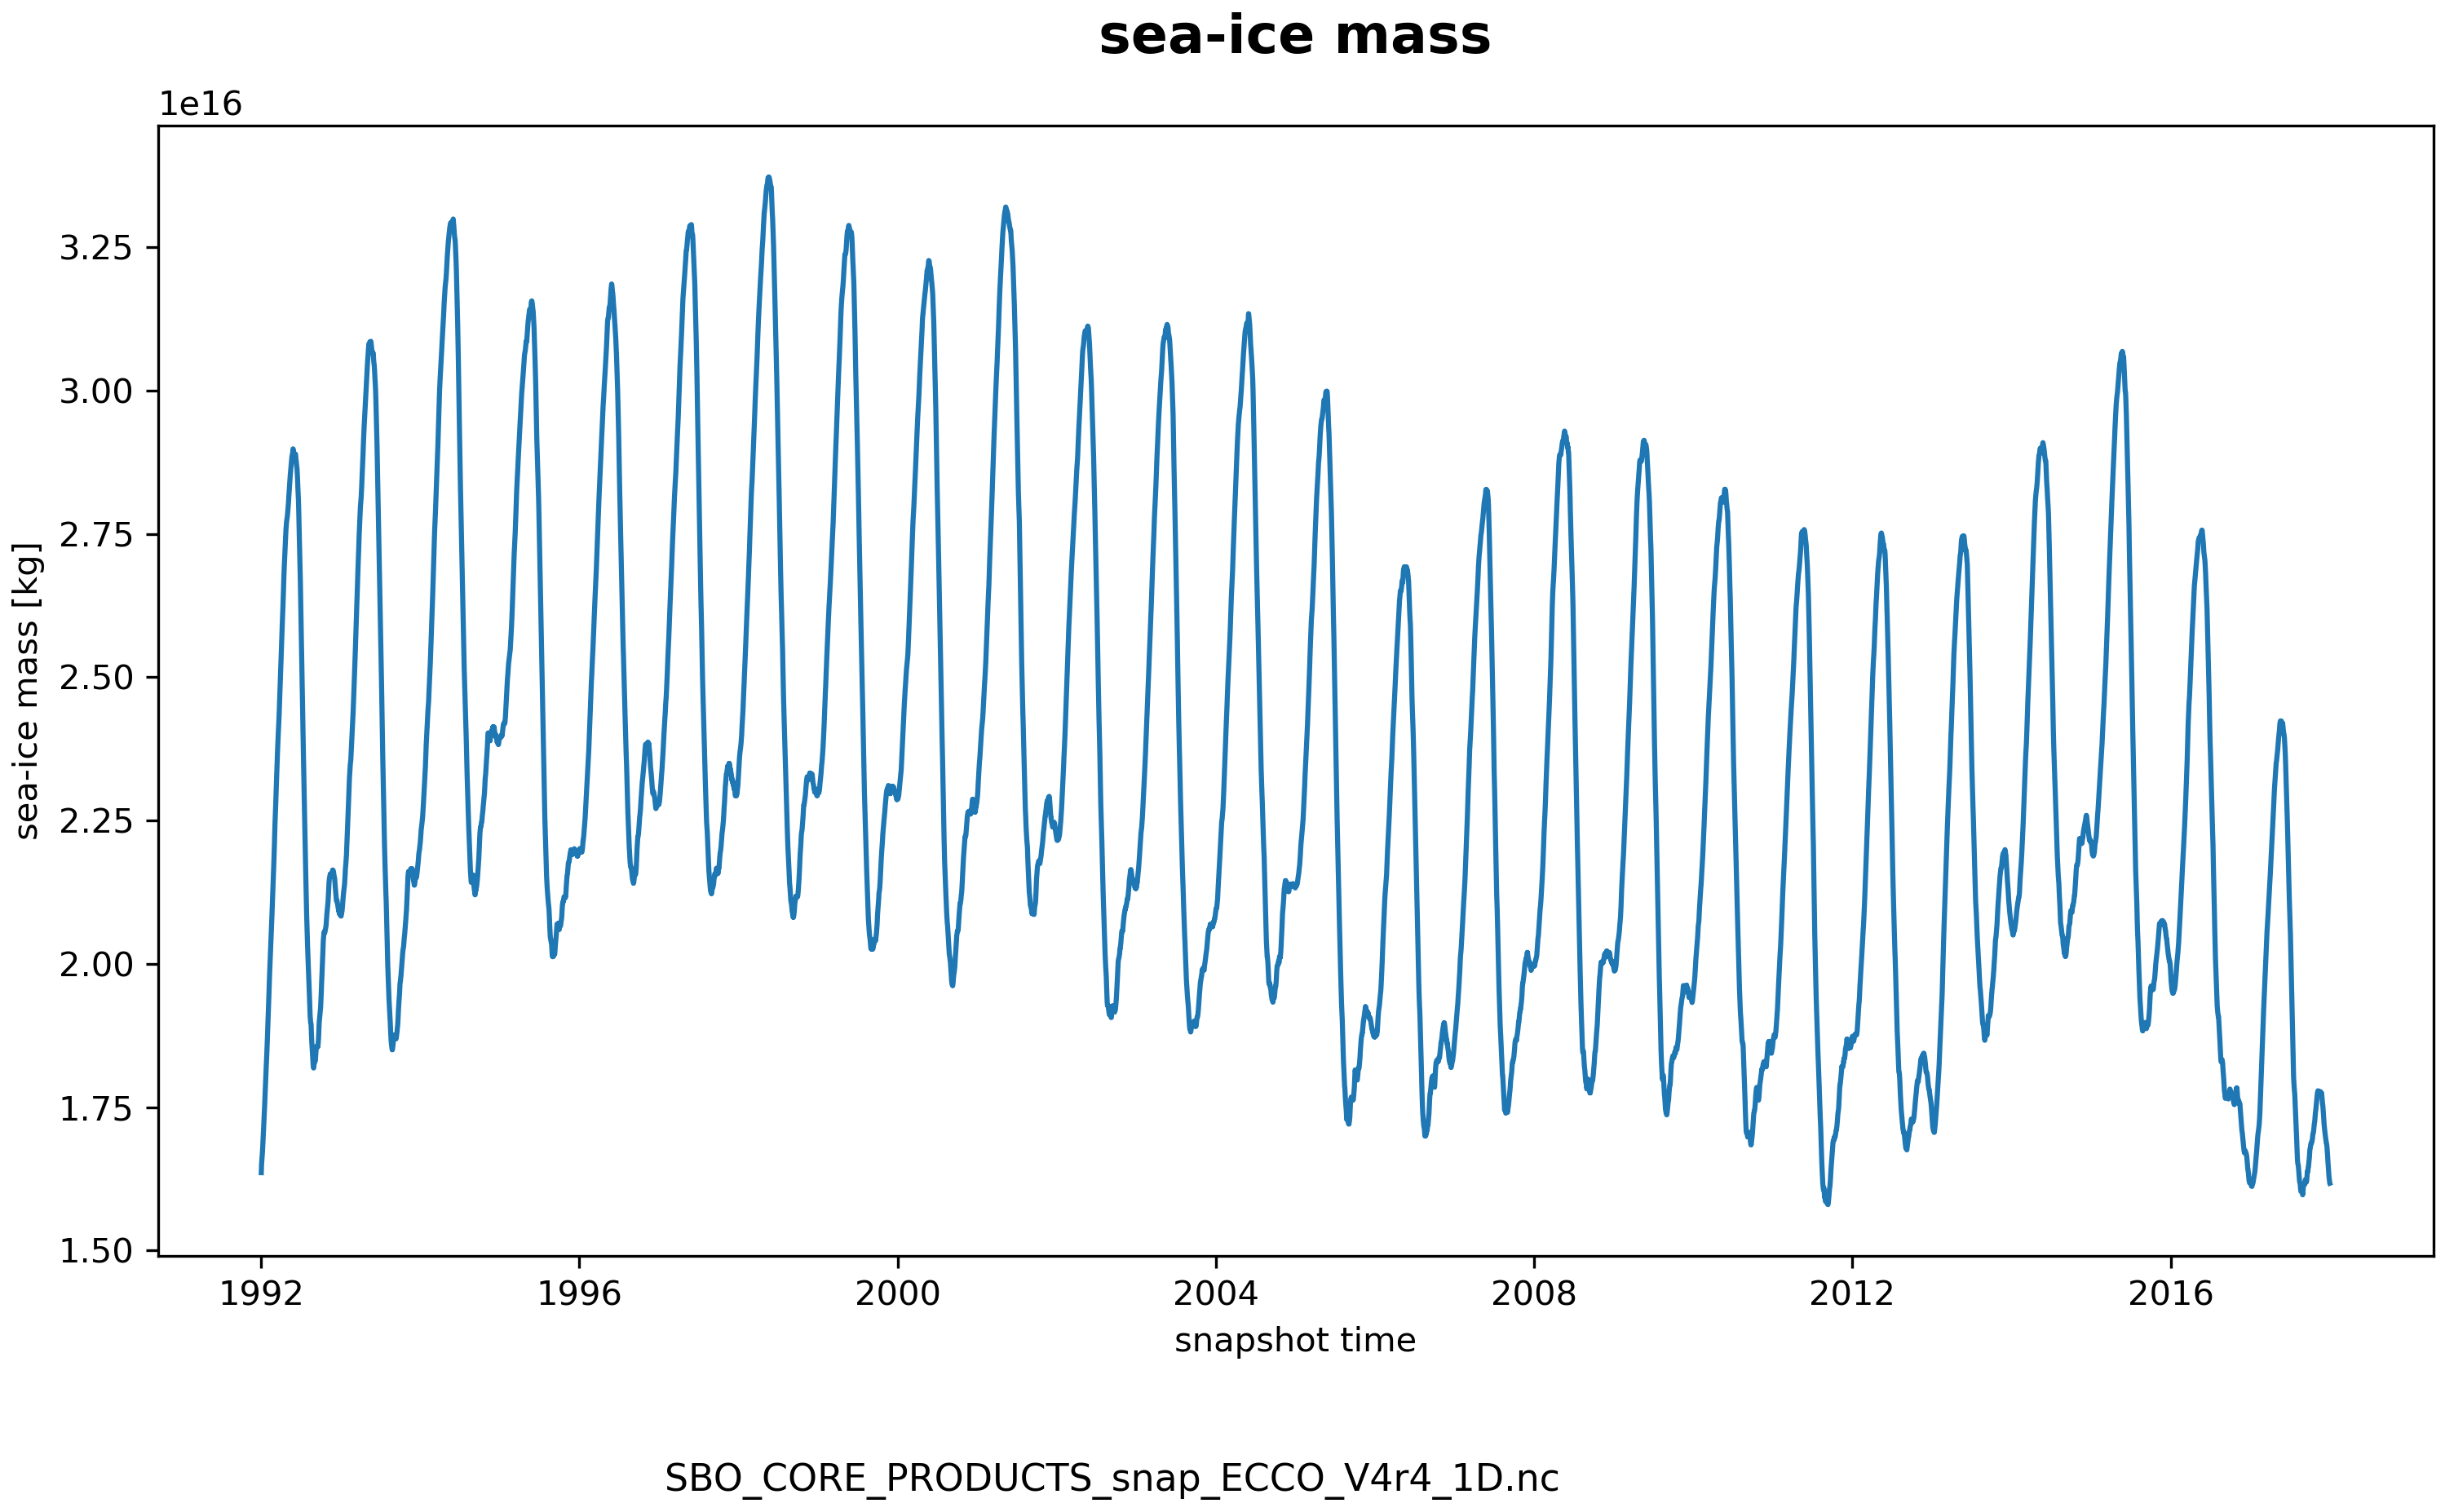
\includegraphics[scale=0.55]{../images/plots/v4r4/oneD_plots/SBO_Core_Products/mass_si.png}
\caption{Dataset: SBO\_CORE\_PRODUCTS, Variable: mass\_si}
\label{tab:table-SBO_CORE_PRODUCTS_mass_si-Plot}
\end{figure}
\newpage
\pagebreak
\subsubsection{1D Variable: sboarea}
\begin{longtable}{|m{0.06\textwidth}|m{0.3\textwidth}|m{0.45\textwidth}|m{0.12\textwidth}|}
\caption{Attributes description of the variable 'sboarea' from SBO\_CORE\_PRODUCTS's  dataset.}
\label{tab:table-SBO_CORE_PRODUCTS_sboarea} \\ 
\hline \endhead \hline \endfoot
\rowcolor{lightgray} \textbf{Storage Type} & \textbf{Variable Name} & \textbf{Description} & \textbf{Unit} \\ \hline
float64 & sboarea & Surface area of oceans & m2 \\ \hline
\multicolumn{4}{|c|}{\cellcolor{lightgray}{\textbf{Description of the variable in Common Data language (CDL)}}} \\ \hline
\multicolumn{4}{|c|}{\fontfamily{lmtt}\selectfont{\makecell{\parbox{.95\textwidth}{\vspace*{0.25cm} \footnotesize{float64 sboarea(time)\\
\hspace*{0.5cm}sboarea: \_FillValue = 9.969209968386869e+36\\
\hspace*{0.5cm}sboarea: coordinates = time\\
\hspace*{0.5cm}sboarea: coverage\_content\_type = modelResult\\
\hspace*{0.5cm}sboarea: long\_name = surface area of oceans\\
\hspace*{0.5cm}sboarea: units = m2\\
\hspace*{0.5cm}sboarea: valid\_max = 358013861149443.5\\
\hspace*{0.5cm}sboarea: valid\_min = 358013861149443.5\\
}}}}} \\ \hline
\rowcolor{lightgray} \multicolumn{4}{|c|}{\textbf{Comments}} \\ \hline
\multicolumn{4}{|p{1\textwidth}|}{\footnotesize{{Note: ocean surface area is constant but provided as time series for convenience}}} \\ \hline
\end{longtable}

\begin{figure}[H]
\centering
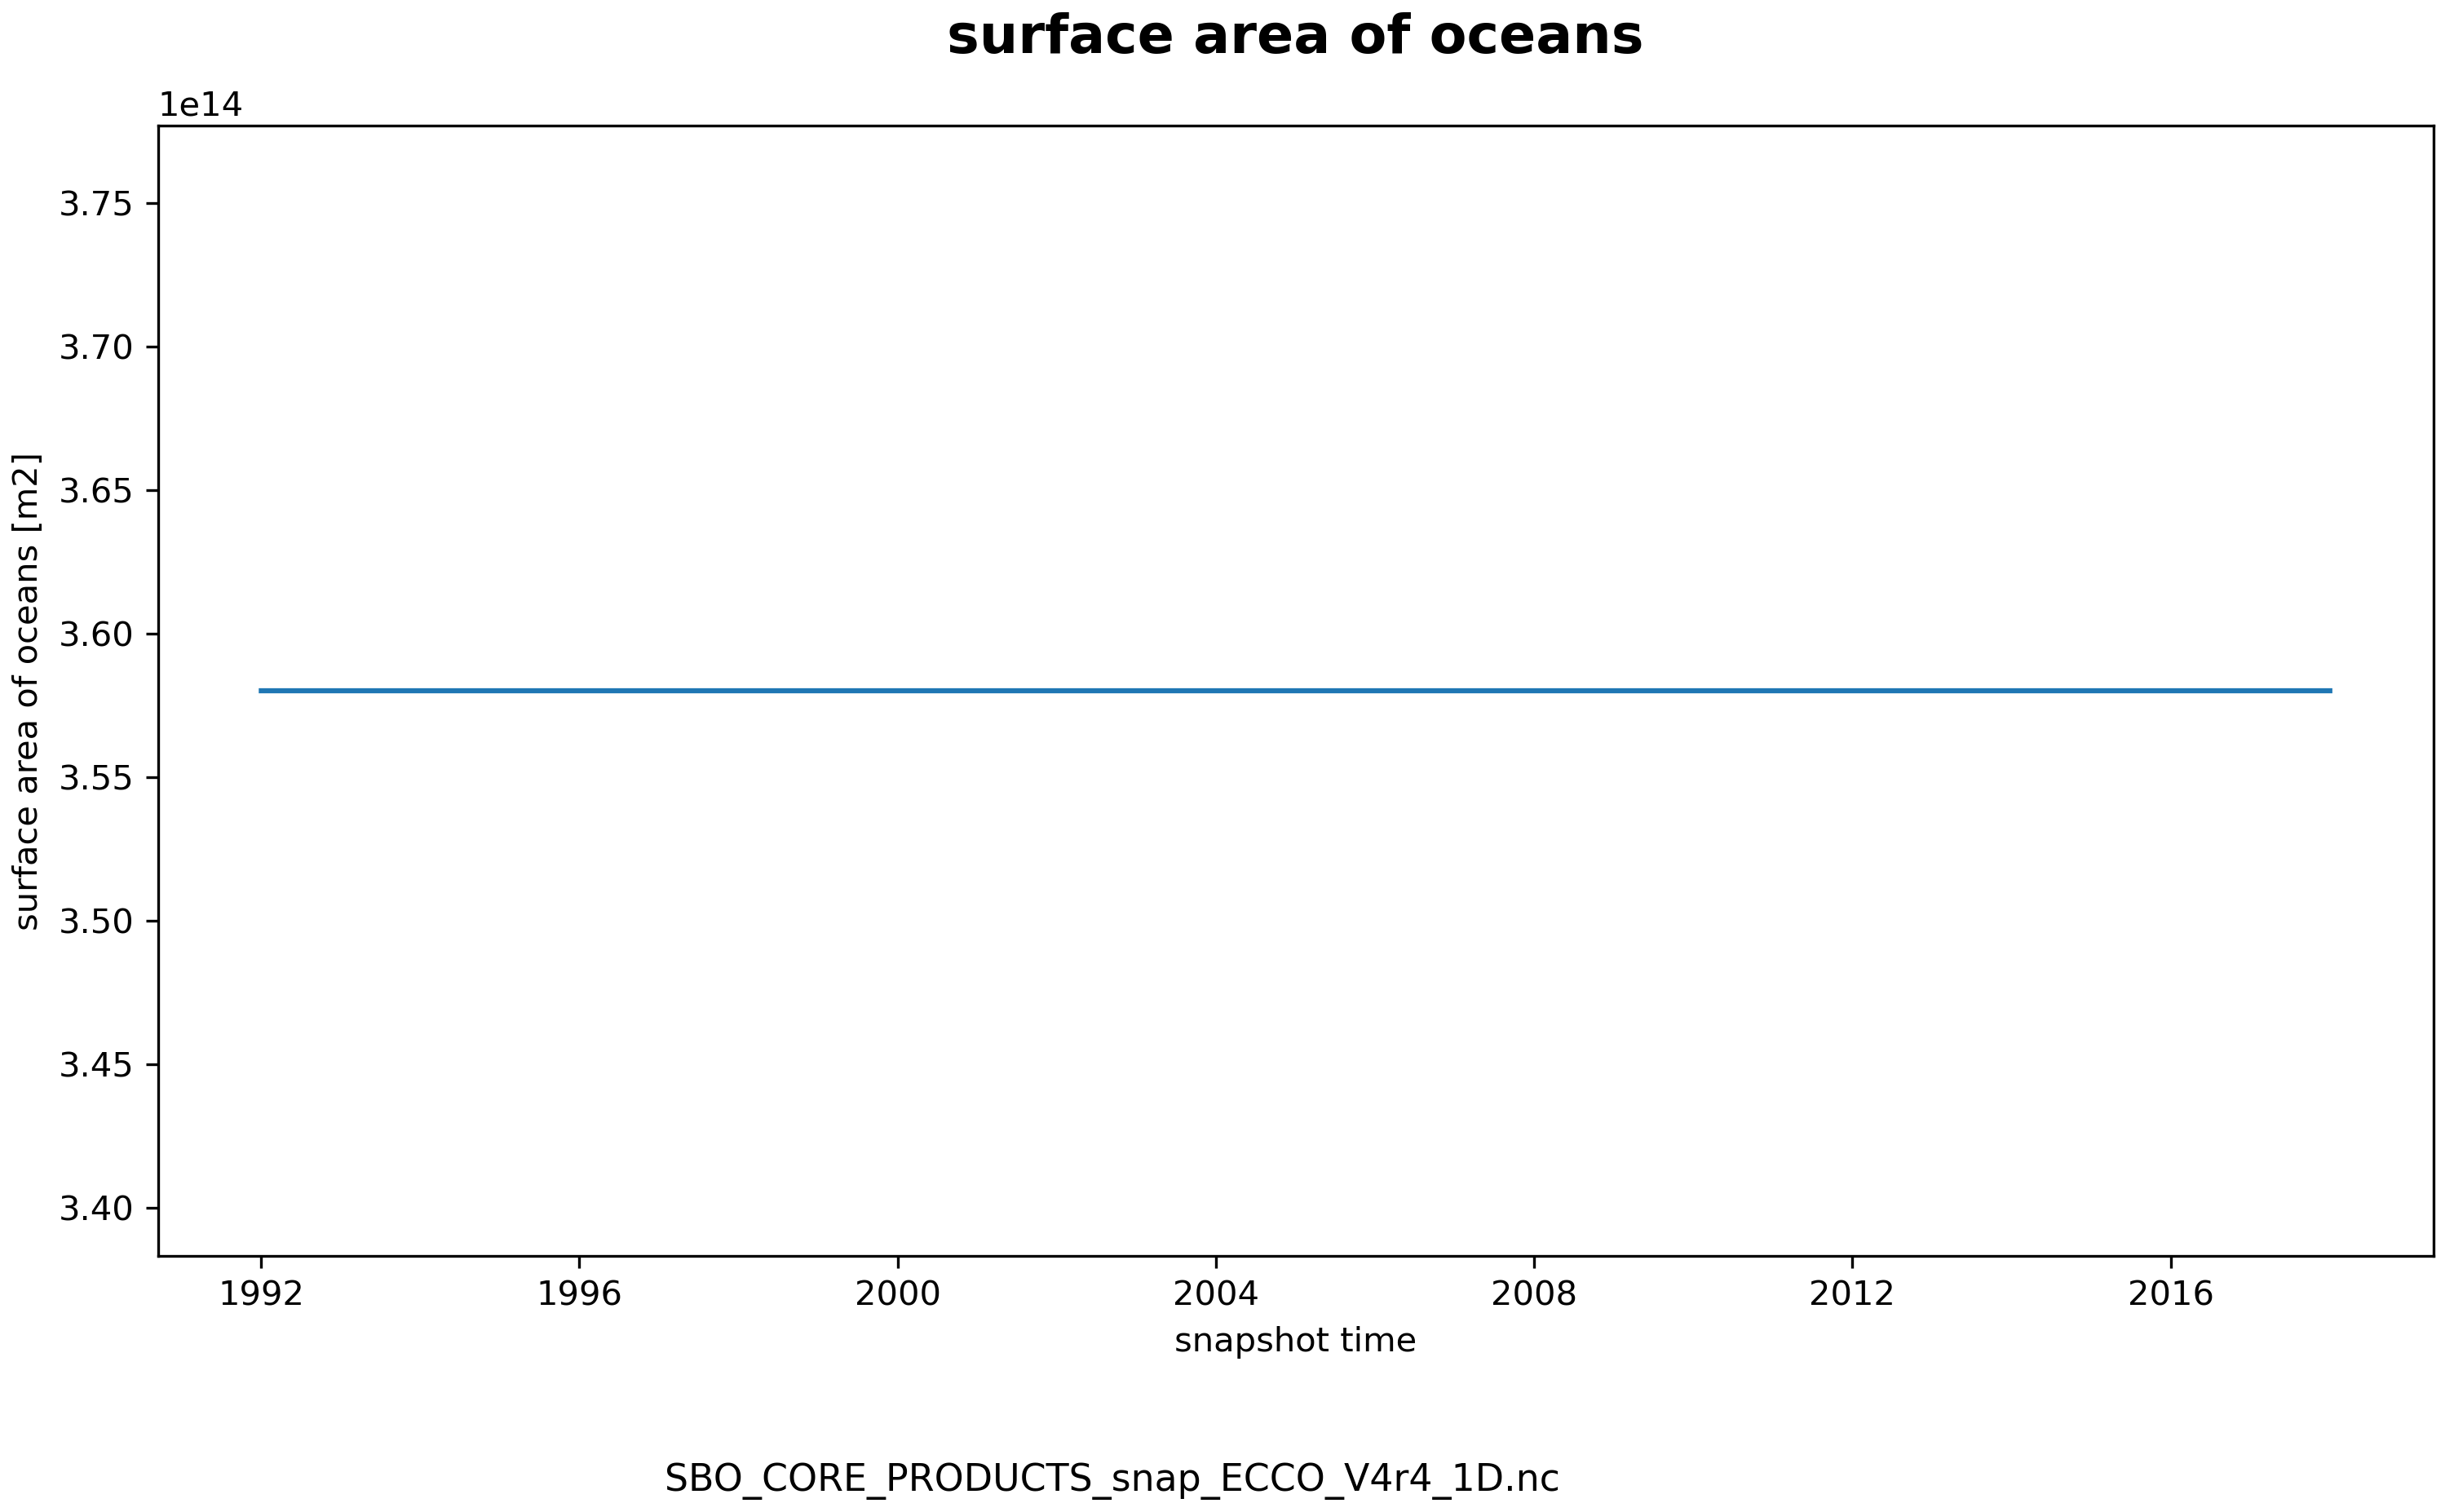
\includegraphics[scale=0.55]{../images/plots/v4r4/oneD_plots/SBO_Core_Products/sboarea.png}
\caption{Dataset: SBO\_CORE\_PRODUCTS, Variable: sboarea}
\label{tab:table-SBO_CORE_PRODUCTS_sboarea-Plot}
\end{figure}
\newpage
\pagebreak
\subsubsection{1D Variable: xcom}
\begin{longtable}{|m{0.06\textwidth}|m{0.3\textwidth}|m{0.45\textwidth}|m{0.12\textwidth}|}
\caption{Attributes description of the variable 'xcom' from SBO\_CORE\_PRODUCTS's  dataset.}
\label{tab:table-SBO_CORE_PRODUCTS_xcom} \\ 
\hline \endhead \hline \endfoot
\rowcolor{lightgray} \textbf{Storage Type} & \textbf{Variable Name} & \textbf{Description} & \textbf{Unit} \\ \hline
float64 & xcom & X-comp of center-of-mass of ocean & m \\ \hline
\multicolumn{4}{|c|}{\cellcolor{lightgray}{\textbf{Description of the variable in Common Data language (CDL)}}} \\ \hline
\multicolumn{4}{|c|}{\fontfamily{lmtt}\selectfont{\makecell{\parbox{.95\textwidth}{\vspace*{0.25cm} \footnotesize{float64 xcom(time)\\
\hspace*{0.5cm}xcom: \_FillValue = 9.969209968386869e+36\\
\hspace*{0.5cm}xcom: coordinates = time\\
\hspace*{0.5cm}xcom: coverage\_content\_type = modelResult\\
\hspace*{0.5cm}xcom: long\_name = x-comp of center-of-mass of ocean\\
\hspace*{0.5cm}xcom: units = m\\
\hspace*{0.5cm}xcom: valid\_max = -763667.0104211655\\
\hspace*{0.5cm}xcom: valid\_min = -763730.0399730895\\
}}}}} \\ \hline
\rowcolor{lightgray} \multicolumn{4}{|c|}{\textbf{Comments}} \\ \hline
\multicolumn{4}{|p{1\textwidth}|}{\footnotesize{{N/a}}} \\ \hline
\end{longtable}

\begin{figure}[H]
\centering
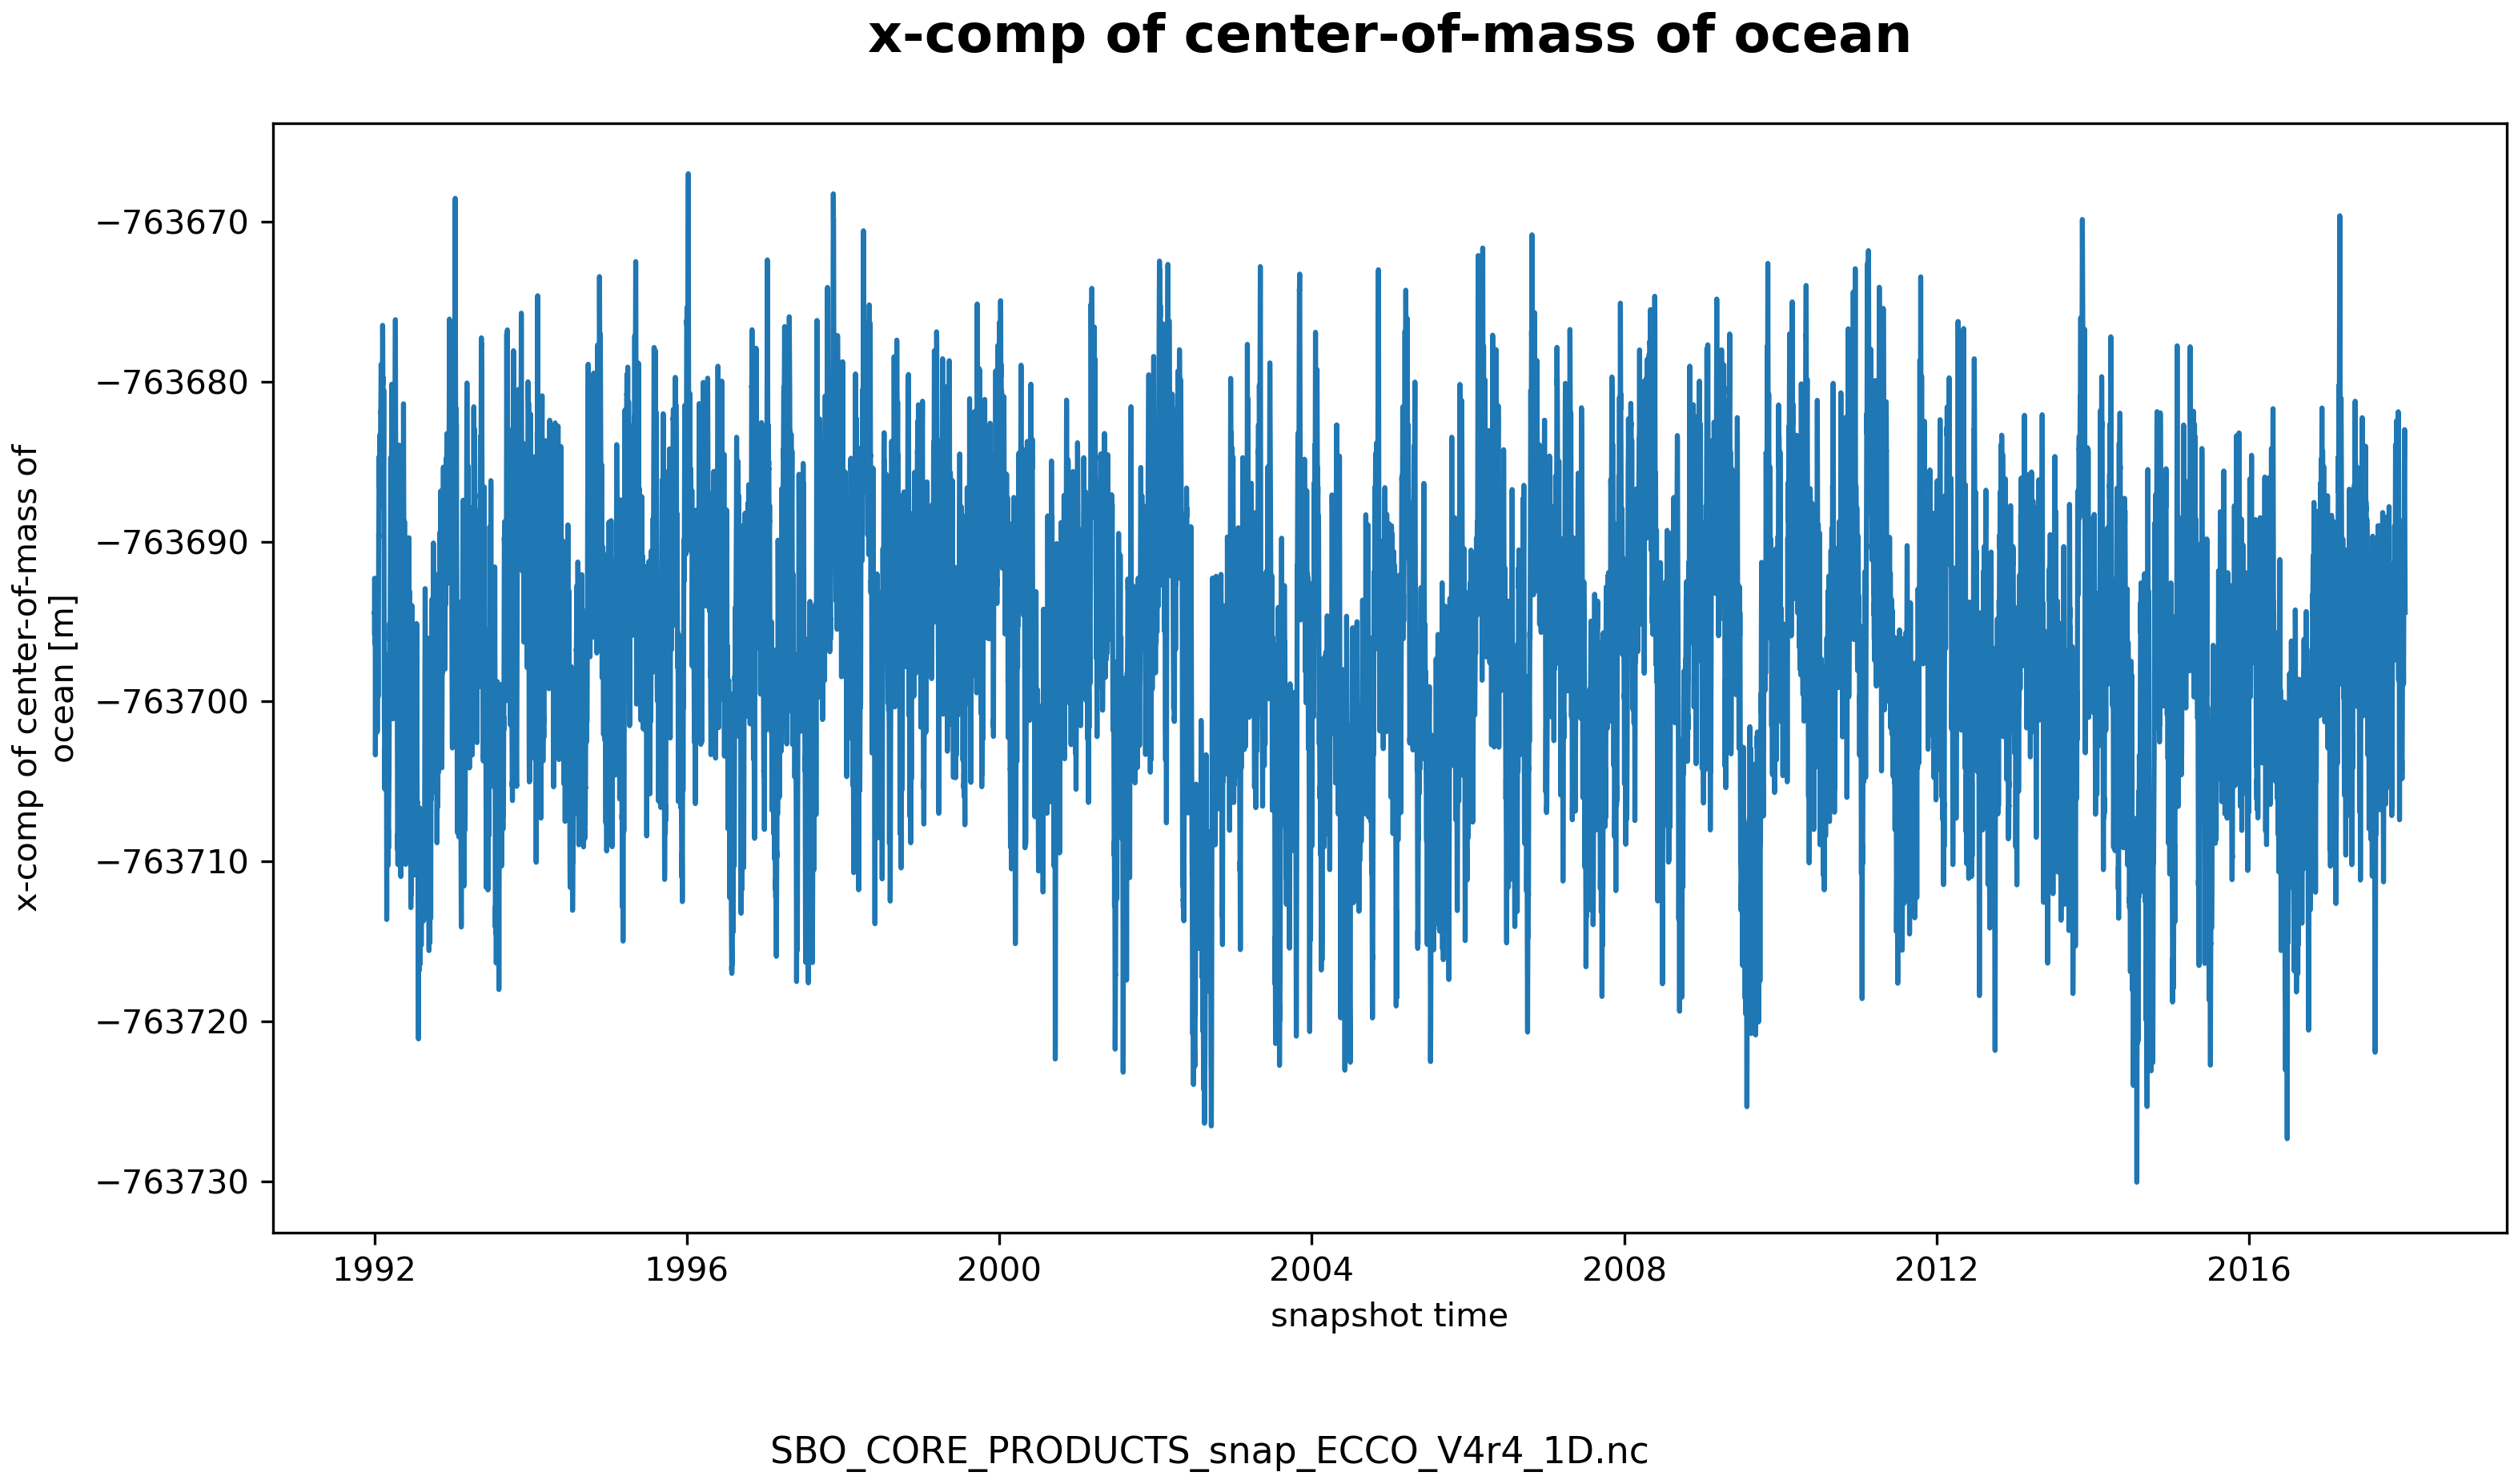
\includegraphics[scale=0.55]{../images/plots/v4r4/oneD_plots/SBO_Core_Products/xcom.png}
\caption{Dataset: SBO\_CORE\_PRODUCTS, Variable: xcom}
\label{tab:table-SBO_CORE_PRODUCTS_xcom-Plot}
\end{figure}
\newpage
\pagebreak
\subsubsection{1D Variable: xcom\_fw}
\begin{longtable}{|m{0.06\textwidth}|m{0.3\textwidth}|m{0.45\textwidth}|m{0.12\textwidth}|}
\caption{Attributes description of the variable 'xcom\_fw' from SBO\_CORE\_PRODUCTS's  dataset.}
\label{tab:table-SBO_CORE_PRODUCTS_xcom_fw} \\ 
\hline \endhead \hline \endfoot
\rowcolor{lightgray} \textbf{Storage Type} & \textbf{Variable Name} & \textbf{Description} & \textbf{Unit} \\ \hline
float64 & xcom\_fw & X-comp of center-of-mass of freshwater flux & m \\ \hline
\multicolumn{4}{|c|}{\cellcolor{lightgray}{\textbf{Description of the variable in Common Data language (CDL)}}} \\ \hline
\multicolumn{4}{|c|}{\fontfamily{lmtt}\selectfont{\makecell{\parbox{.95\textwidth}{\vspace*{0.25cm} \footnotesize{float64 xcom\_fw(time)\\
\hspace*{0.5cm}xcom\_fw: \_FillValue = 9.969209968386869e+36\\
\hspace*{0.5cm}xcom\_fw: coordinates = time\\
\hspace*{0.5cm}xcom\_fw: coverage\_content\_type = modelResult\\
\hspace*{0.5cm}xcom\_fw: long\_name = x-comp of center-of-mass of freshwater flux\\
\hspace*{0.5cm}xcom\_fw: units = m\\
\hspace*{0.5cm}xcom\_fw: valid\_max = -573864.6948562652\\
\hspace*{0.5cm}xcom\_fw: valid\_min = -573864.6948562702\\
}}}}} \\ \hline
\rowcolor{lightgray} \multicolumn{4}{|c|}{\textbf{Comments}} \\ \hline
\multicolumn{4}{|p{1\textwidth}|}{\footnotesize{{N/a}}} \\ \hline
\end{longtable}

\begin{figure}[H]
\centering
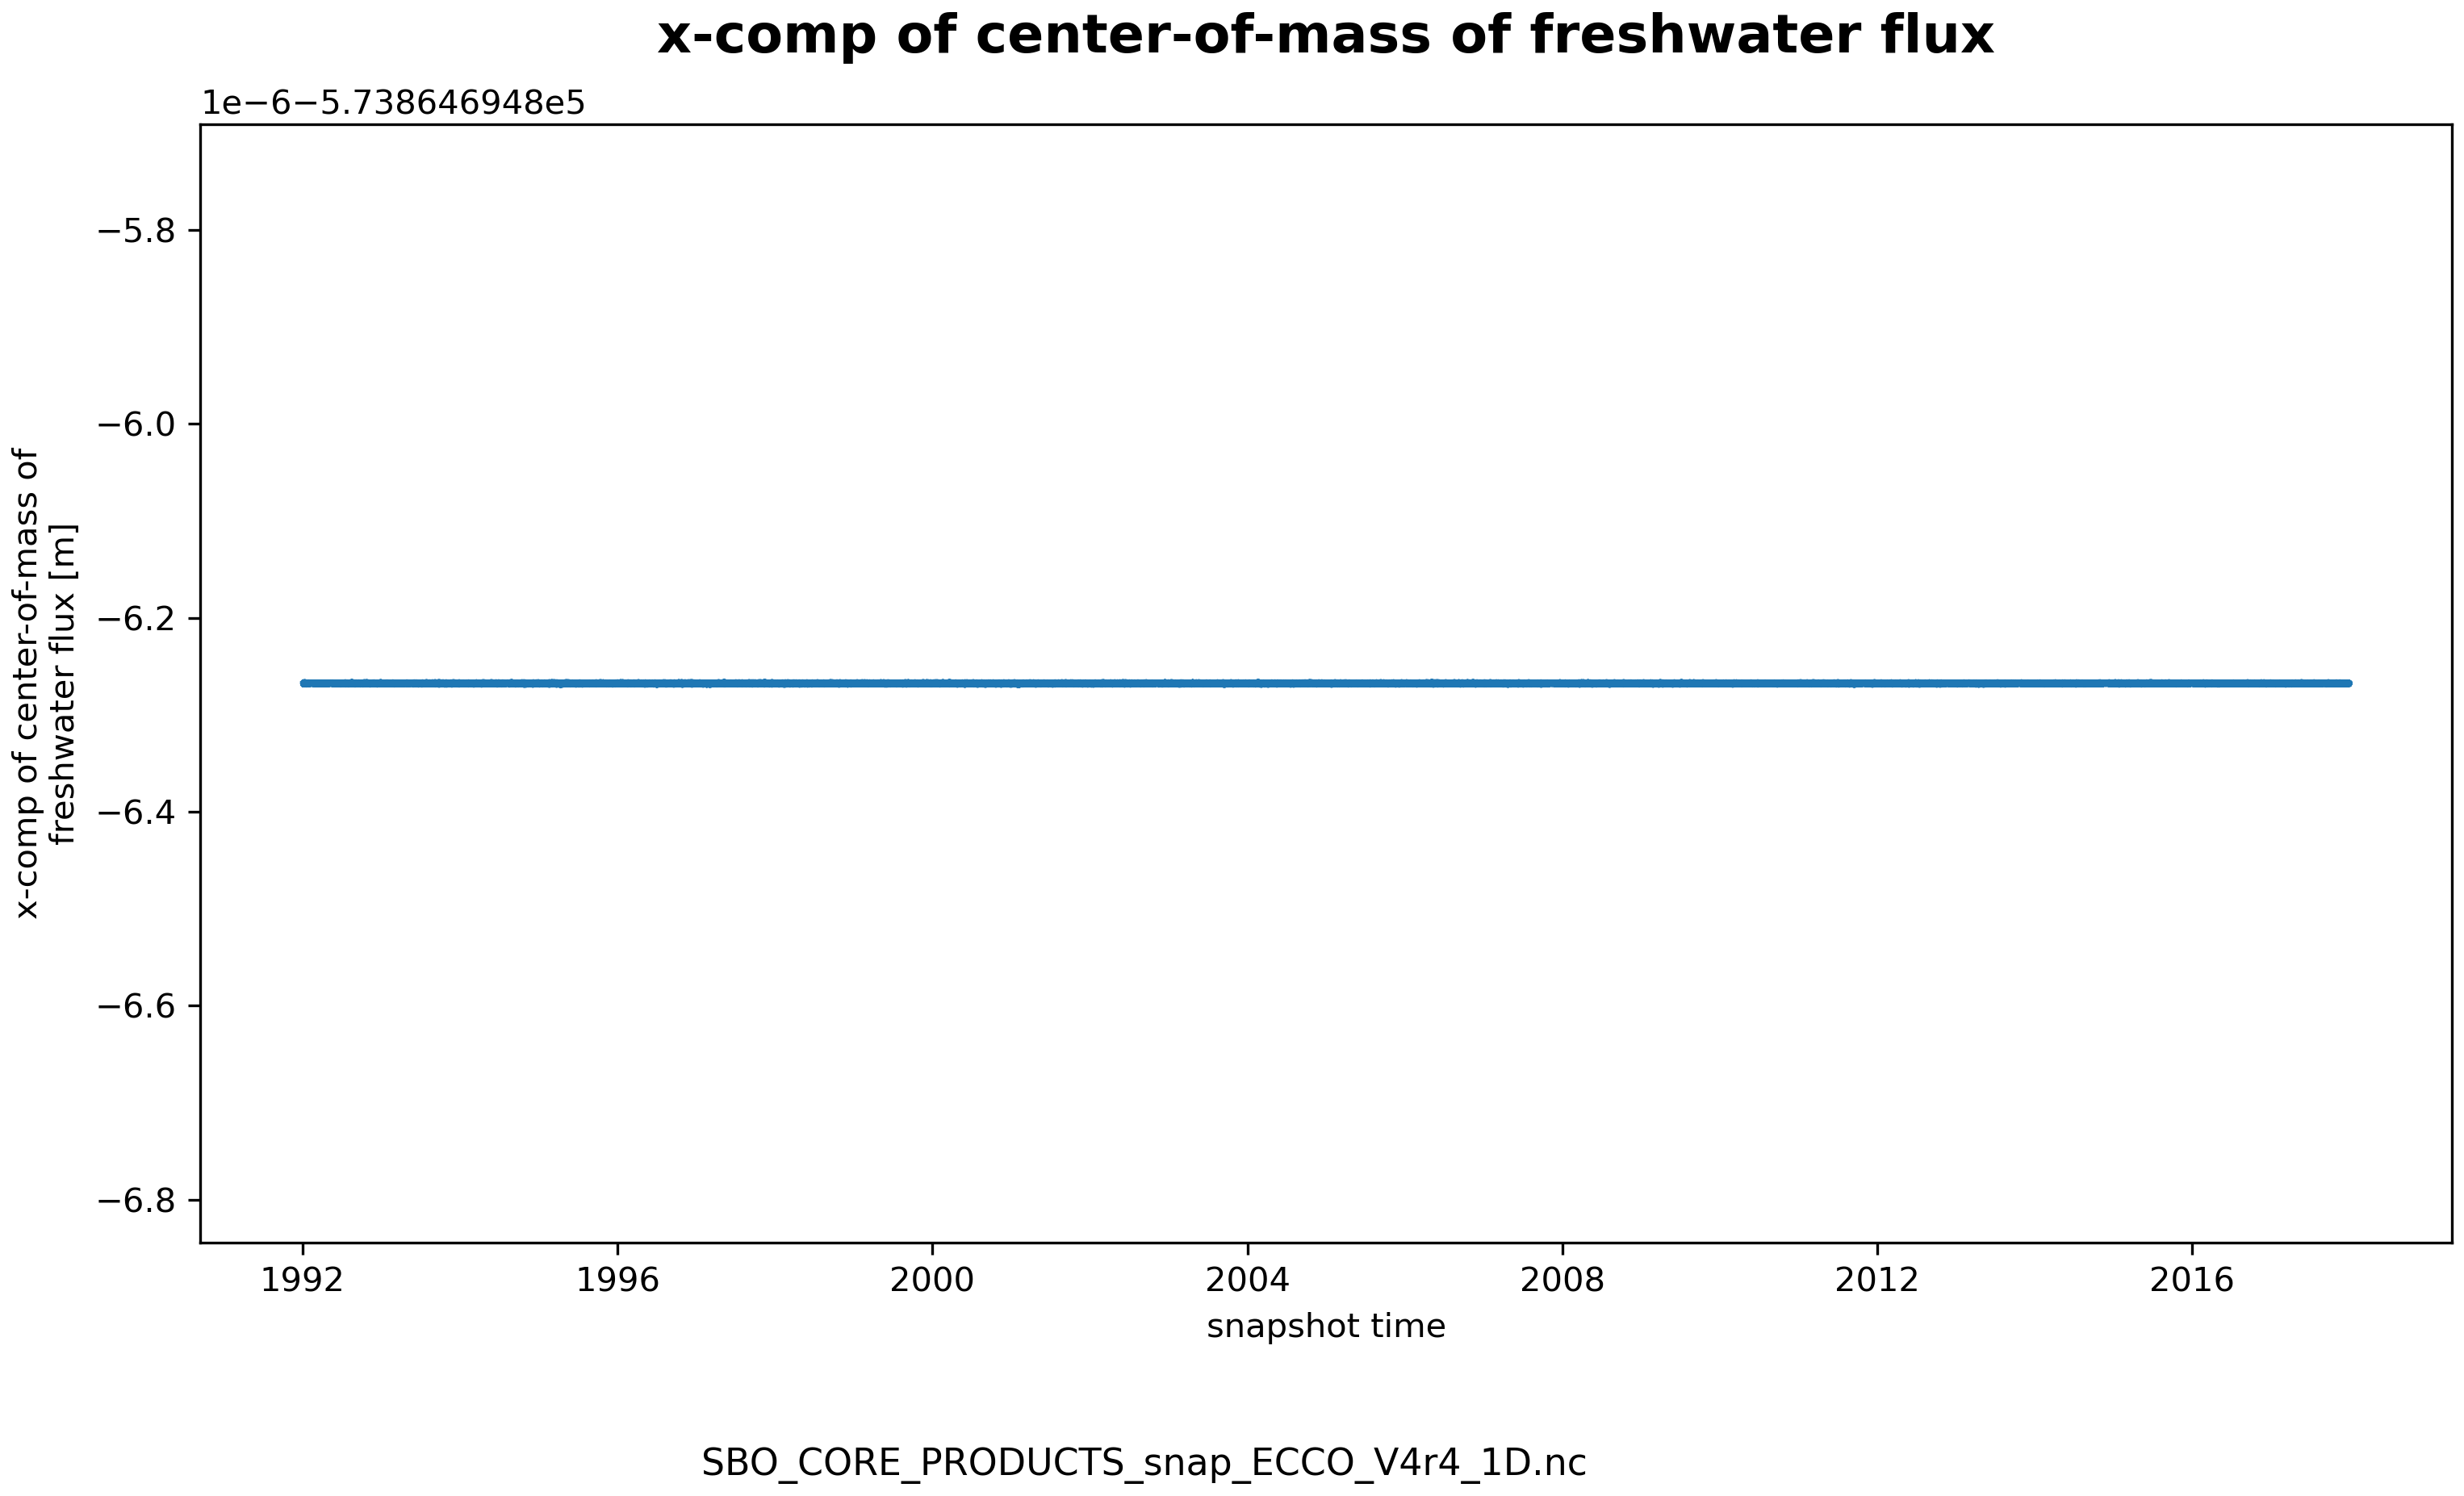
\includegraphics[scale=0.55]{../images/plots/v4r4/oneD_plots/SBO_Core_Products/xcom_fw.png}
\caption{Dataset: SBO\_CORE\_PRODUCTS, Variable: xcom\_fw}
\label{tab:table-SBO_CORE_PRODUCTS_xcom_fw-Plot}
\end{figure}
\newpage
\pagebreak
\subsubsection{1D Variable: xoamc}
\begin{longtable}{|m{0.06\textwidth}|m{0.3\textwidth}|m{0.45\textwidth}|m{0.12\textwidth}|}
\caption{Attributes description of the variable 'xoamc' from SBO\_CORE\_PRODUCTS's  dataset.}
\label{tab:table-SBO_CORE_PRODUCTS_xoamc} \\ 
\hline \endhead \hline \endfoot
\rowcolor{lightgray} \textbf{Storage Type} & \textbf{Variable Name} & \textbf{Description} & \textbf{Unit} \\ \hline
float64 & xoamc & X-comp of oceanic angular momentum due to currents & kg m2 s-1 \\ \hline
\multicolumn{4}{|c|}{\cellcolor{lightgray}{\textbf{Description of the variable in Common Data language (CDL)}}} \\ \hline
\multicolumn{4}{|c|}{\fontfamily{lmtt}\selectfont{\makecell{\parbox{.95\textwidth}{\vspace*{0.25cm} \footnotesize{float64 xoamc(time)\\
\hspace*{0.5cm}xoamc: \_FillValue = 9.969209968386869e+36\\
\hspace*{0.5cm}xoamc: coordinates = time\\
\hspace*{0.5cm}xoamc: coverage\_content\_type = modelResult\\
\hspace*{0.5cm}xoamc: long\_name = x-comp of oceanic angular momentum due to currents\\
\hspace*{0.5cm}xoamc: units = kg m2 s-1\\
\hspace*{0.5cm}xoamc: valid\_max = 2.555331552045857e+24\\
\hspace*{0.5cm}xoamc: valid\_min = -3.783733447704127e+24\\
}}}}} \\ \hline
\rowcolor{lightgray} \multicolumn{4}{|c|}{\textbf{Comments}} \\ \hline
\multicolumn{4}{|p{1\textwidth}|}{\footnotesize{{N/a}}} \\ \hline
\end{longtable}

\begin{figure}[H]
\centering
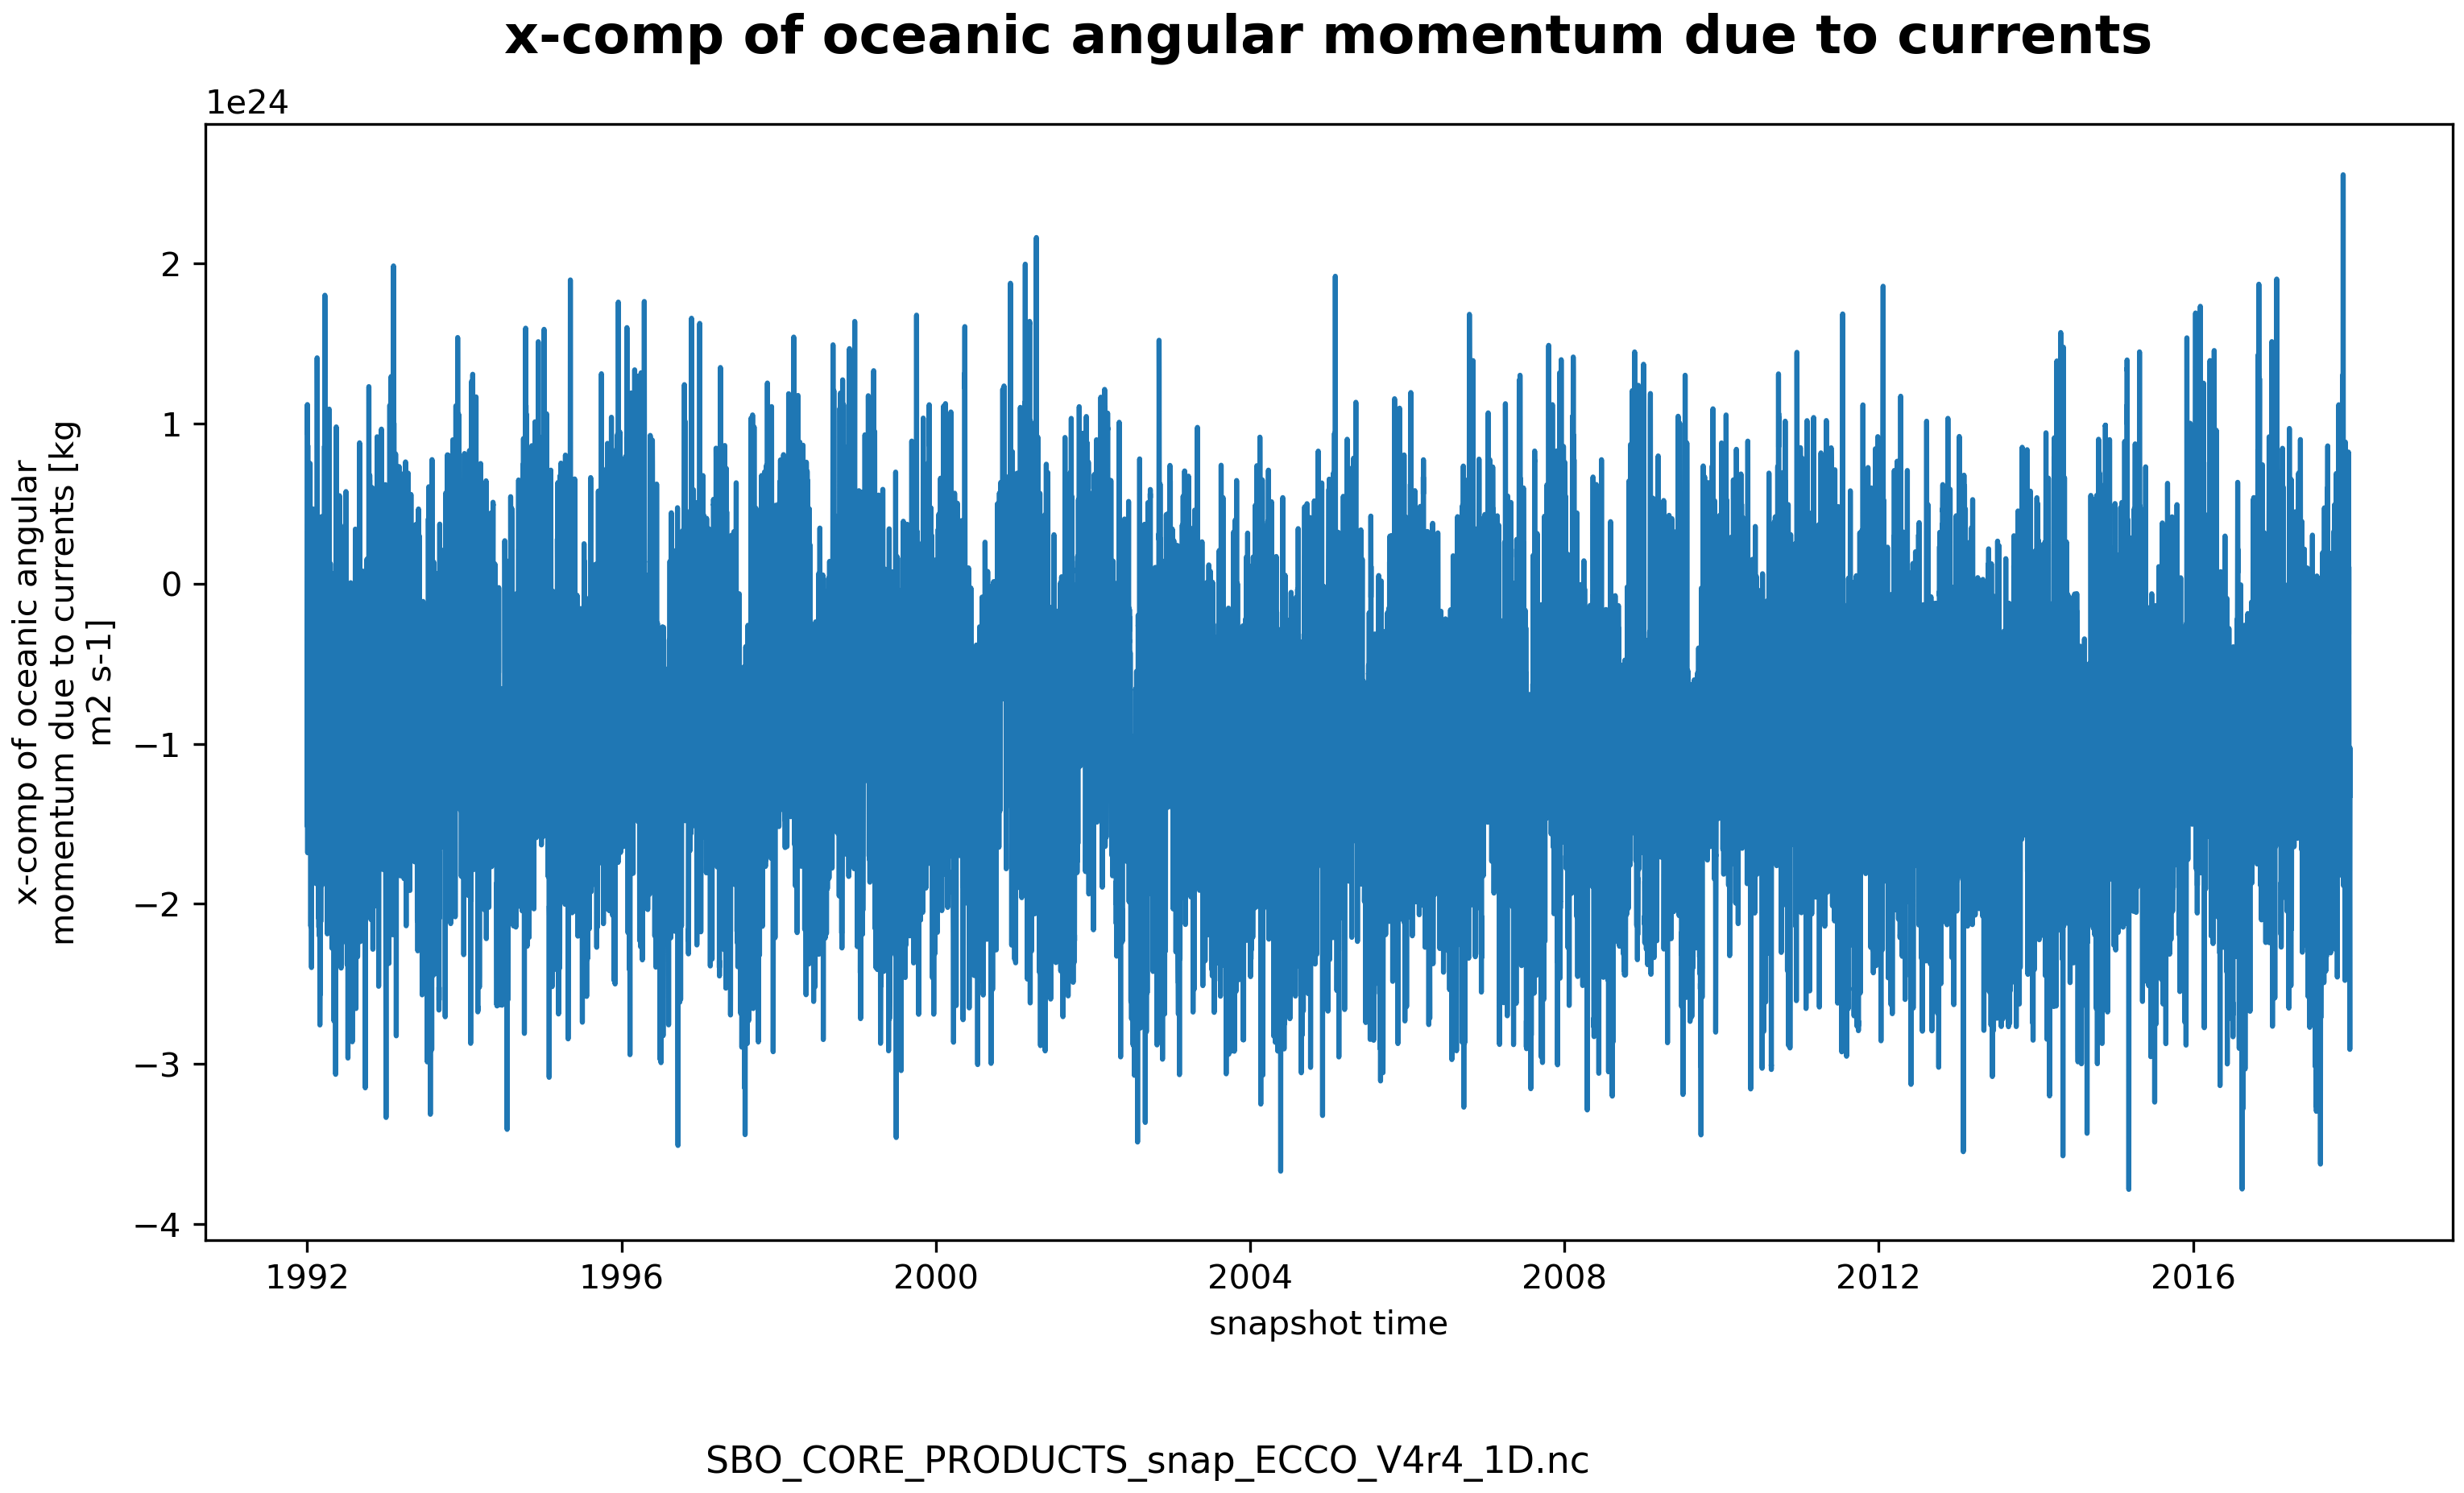
\includegraphics[scale=0.55]{../images/plots/v4r4/oneD_plots/SBO_Core_Products/xoamc.png}
\caption{Dataset: SBO\_CORE\_PRODUCTS, Variable: xoamc}
\label{tab:table-SBO_CORE_PRODUCTS_xoamc-Plot}
\end{figure}
\newpage
\pagebreak
\subsubsection{1D Variable: xoamc\_si}
\begin{longtable}{|m{0.06\textwidth}|m{0.3\textwidth}|m{0.45\textwidth}|m{0.12\textwidth}|}
\caption{Attributes description of the variable 'xoamc\_si' from SBO\_CORE\_PRODUCTS's  dataset.}
\label{tab:table-SBO_CORE_PRODUCTS_xoamc_si} \\ 
\hline \endhead \hline \endfoot
\rowcolor{lightgray} \textbf{Storage Type} & \textbf{Variable Name} & \textbf{Description} & \textbf{Unit} \\ \hline
float64 & xoamc\_si & X-comp of oceanic angular momentum due to sea-ice motion & kg m2 s-1 \\ \hline
\multicolumn{4}{|c|}{\cellcolor{lightgray}{\textbf{Description of the variable in Common Data language (CDL)}}} \\ \hline
\multicolumn{4}{|c|}{\fontfamily{lmtt}\selectfont{\makecell{\parbox{.95\textwidth}{\vspace*{0.25cm} \footnotesize{float64 xoamc\_si(time)\\
\hspace*{0.5cm}xoamc\_si: \_FillValue = 9.969209968386869e+36\\
\hspace*{0.5cm}xoamc\_si: coordinates = time\\
\hspace*{0.5cm}xoamc\_si: coverage\_content\_type = modelResult\\
\hspace*{0.5cm}xoamc\_si: long\_name = x-comp of oceanic angular momentum due to sea-ice motion\\
\hspace*{0.5cm}xoamc\_si: units = kg m2 s-1\\
\hspace*{0.5cm}xoamc\_si: valid\_max = 1.3721188892065168e+22\\
\hspace*{0.5cm}xoamc\_si: valid\_min = -9.76342837969224e+21\\
}}}}} \\ \hline
\rowcolor{lightgray} \multicolumn{4}{|c|}{\textbf{Comments}} \\ \hline
\multicolumn{4}{|p{1\textwidth}|}{\footnotesize{{N/a}}} \\ \hline
\end{longtable}

\begin{figure}[H]
\centering
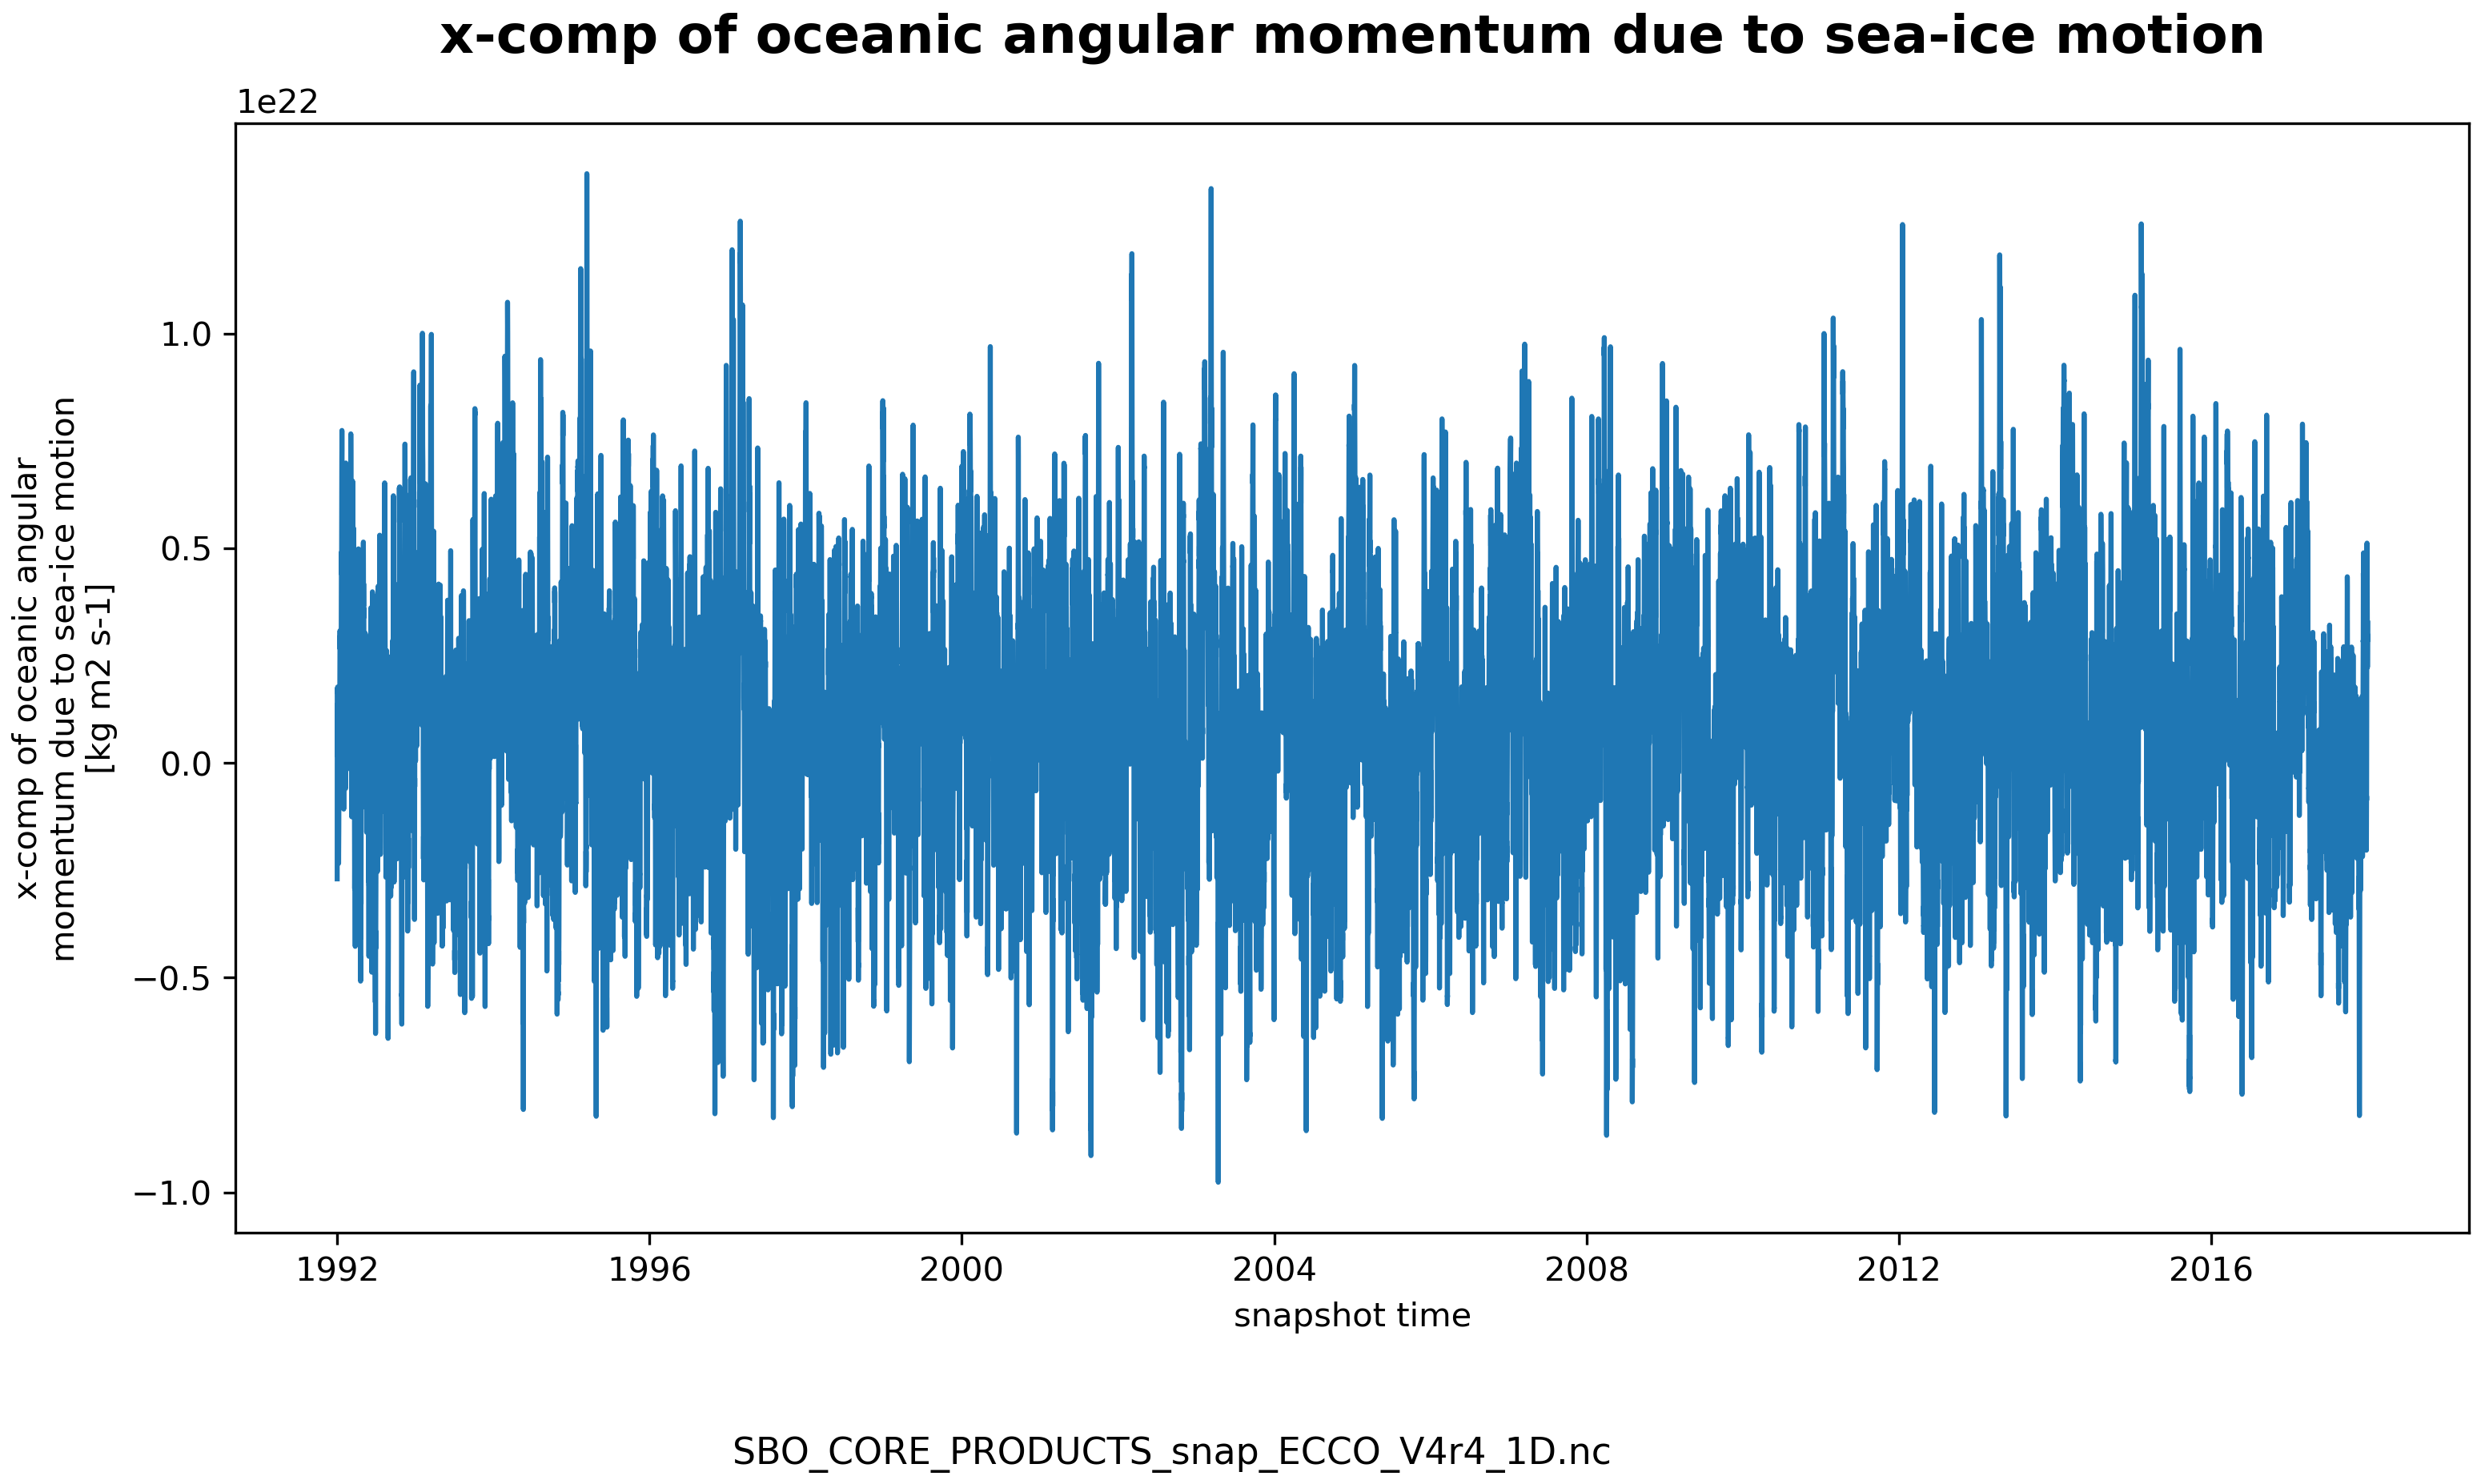
\includegraphics[scale=0.55]{../images/plots/v4r4/oneD_plots/SBO_Core_Products/xoamc_si.png}
\caption{Dataset: SBO\_CORE\_PRODUCTS, Variable: xoamc\_si}
\label{tab:table-SBO_CORE_PRODUCTS_xoamc_si-Plot}
\end{figure}
\newpage
\pagebreak
\subsubsection{1D Variable: xoamp}
\begin{longtable}{|m{0.06\textwidth}|m{0.3\textwidth}|m{0.45\textwidth}|m{0.12\textwidth}|}
\caption{Attributes description of the variable 'xoamp' from SBO\_CORE\_PRODUCTS's  dataset.}
\label{tab:table-SBO_CORE_PRODUCTS_xoamp} \\ 
\hline \endhead \hline \endfoot
\rowcolor{lightgray} \textbf{Storage Type} & \textbf{Variable Name} & \textbf{Description} & \textbf{Unit} \\ \hline
float64 & xoamp & X-comp of oceanic angular momentum due to pressure & kg m2 s-1 \\ \hline
\multicolumn{4}{|c|}{\cellcolor{lightgray}{\textbf{Description of the variable in Common Data language (CDL)}}} \\ \hline
\multicolumn{4}{|c|}{\fontfamily{lmtt}\selectfont{\makecell{\parbox{.95\textwidth}{\vspace*{0.25cm} \footnotesize{float64 xoamp(time)\\
\hspace*{0.5cm}xoamp: \_FillValue = 9.969209968386869e+36\\
\hspace*{0.5cm}xoamp: coordinates = time\\
\hspace*{0.5cm}xoamp: coverage\_content\_type = modelResult\\
\hspace*{0.5cm}xoamp: long\_name = x-comp of oceanic angular momentum due to pressure\\
\hspace*{0.5cm}xoamp: units = kg m2 s-1\\
\hspace*{0.5cm}xoamp: valid\_max = 1.3546098666231897e+29\\
\hspace*{0.5cm}xoamp: valid\_min = 1.3543642768158851e+29\\
}}}}} \\ \hline
\rowcolor{lightgray} \multicolumn{4}{|c|}{\textbf{Comments}} \\ \hline
\multicolumn{4}{|p{1\textwidth}|}{\footnotesize{{N/a}}} \\ \hline
\end{longtable}

\begin{figure}[H]
\centering
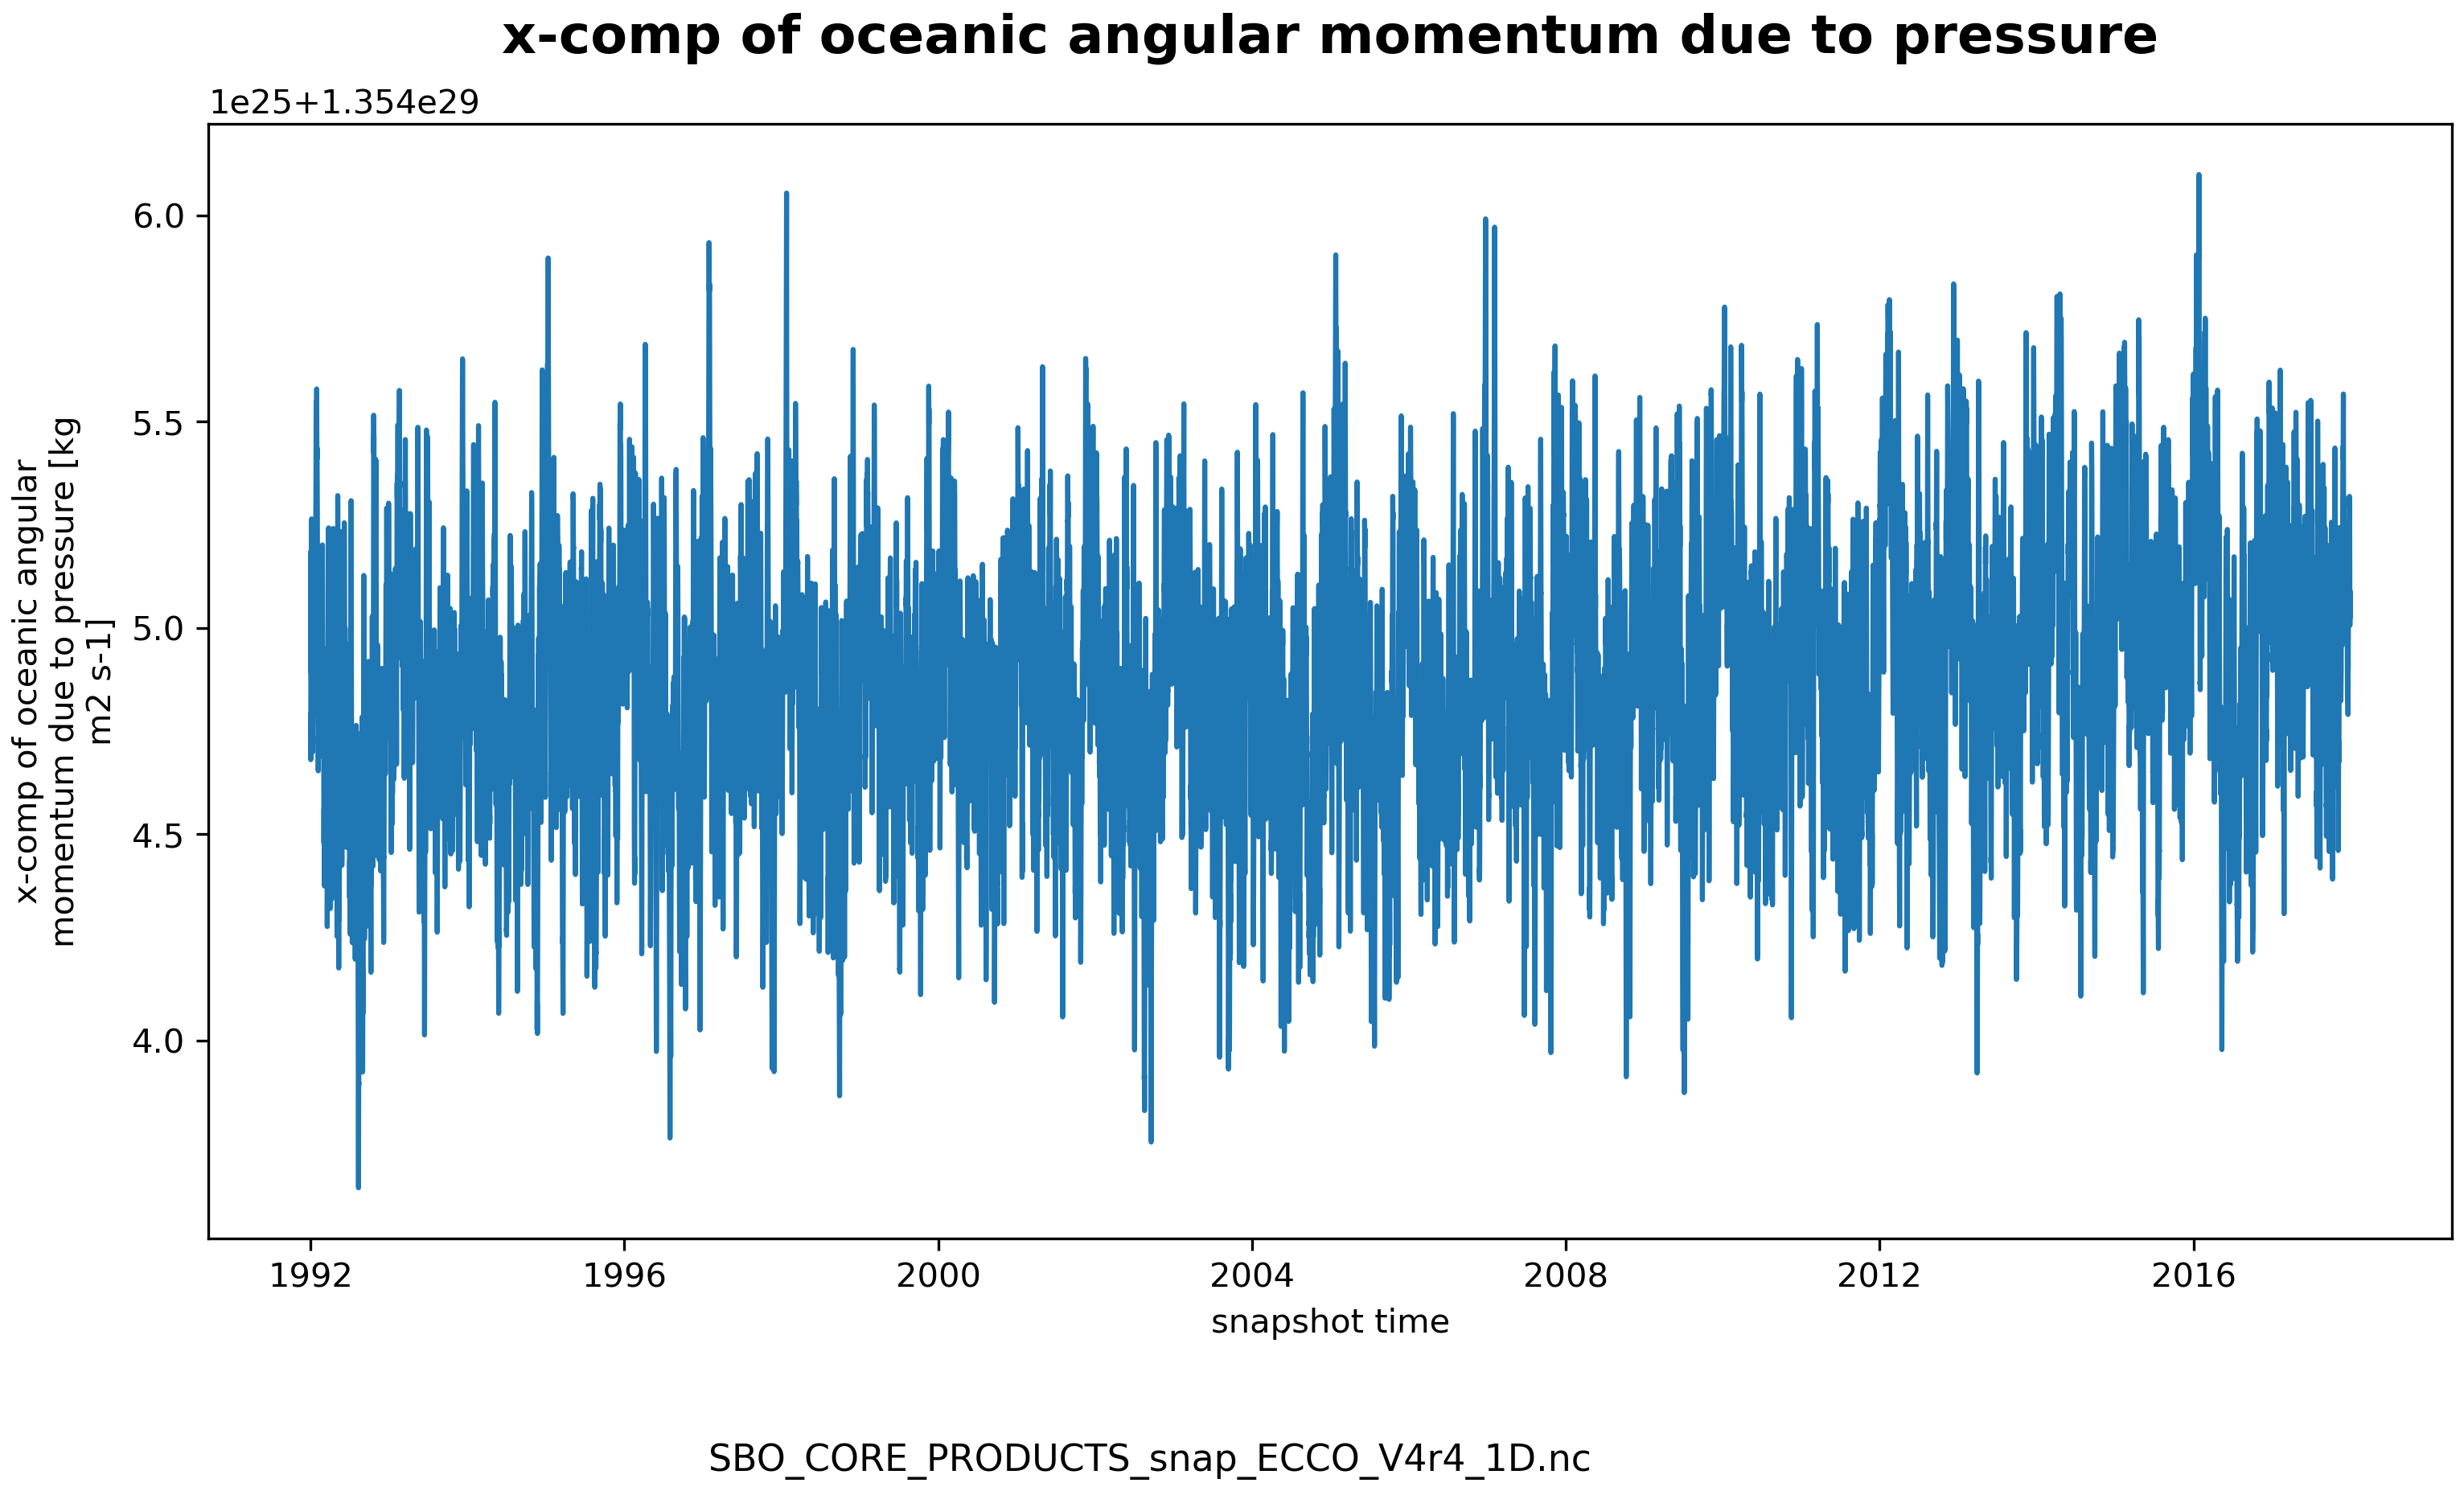
\includegraphics[scale=0.55]{../images/plots/v4r4/oneD_plots/SBO_Core_Products/xoamp.png}
\caption{Dataset: SBO\_CORE\_PRODUCTS, Variable: xoamp}
\label{tab:table-SBO_CORE_PRODUCTS_xoamp-Plot}
\end{figure}
\newpage
\pagebreak
\subsubsection{1D Variable: xoamp\_dsl}
\begin{longtable}{|m{0.06\textwidth}|m{0.3\textwidth}|m{0.45\textwidth}|m{0.12\textwidth}|}
\caption{Attributes description of the variable 'xoamp\_dsl' from SBO\_CORE\_PRODUCTS's  dataset.}
\label{tab:table-SBO_CORE_PRODUCTS_xoamp_dsl} \\ 
\hline \endhead \hline \endfoot
\rowcolor{lightgray} \textbf{Storage Type} & \textbf{Variable Name} & \textbf{Description} & \textbf{Unit} \\ \hline
float64 & xoamp\_dsl & X-comp of oceanic angular momentum due to pressure based on dynamic (ib-corrected) sea level & kg m2 s-1 \\ \hline
\multicolumn{4}{|c|}{\cellcolor{lightgray}{\textbf{Description of the variable in Common Data language (CDL)}}} \\ \hline
\multicolumn{4}{|c|}{\fontfamily{lmtt}\selectfont{\makecell{\parbox{.95\textwidth}{\vspace*{0.25cm} \footnotesize{float64 xoamp\_dsl(time)\\
\hspace*{0.5cm}xoamp\_dsl: \_FillValue = 9.969209968386869e+36\\
\hspace*{0.5cm}xoamp\_dsl: coordinates = time\\
\hspace*{0.5cm}xoamp\_dsl: coverage\_content\_type = modelResult\\
\hspace*{0.5cm}xoamp\_dsl: long\_name = x-comp of oceanic angular momentum due to pressure based on dynamic (IB-corrected) sea level\\
\hspace*{0.5cm}xoamp\_dsl: units = kg m2 s-1\\
\hspace*{0.5cm}xoamp\_dsl: valid\_max = 1.3545518352698056e+29\\
\hspace*{0.5cm}xoamp\_dsl: valid\_min = 1.354440386439953e+29\\
}}}}} \\ \hline
\rowcolor{lightgray} \multicolumn{4}{|c|}{\textbf{Comments}} \\ \hline
\multicolumn{4}{|p{1\textwidth}|}{\footnotesize{{N/a}}} \\ \hline
\end{longtable}

\begin{figure}[H]
\centering
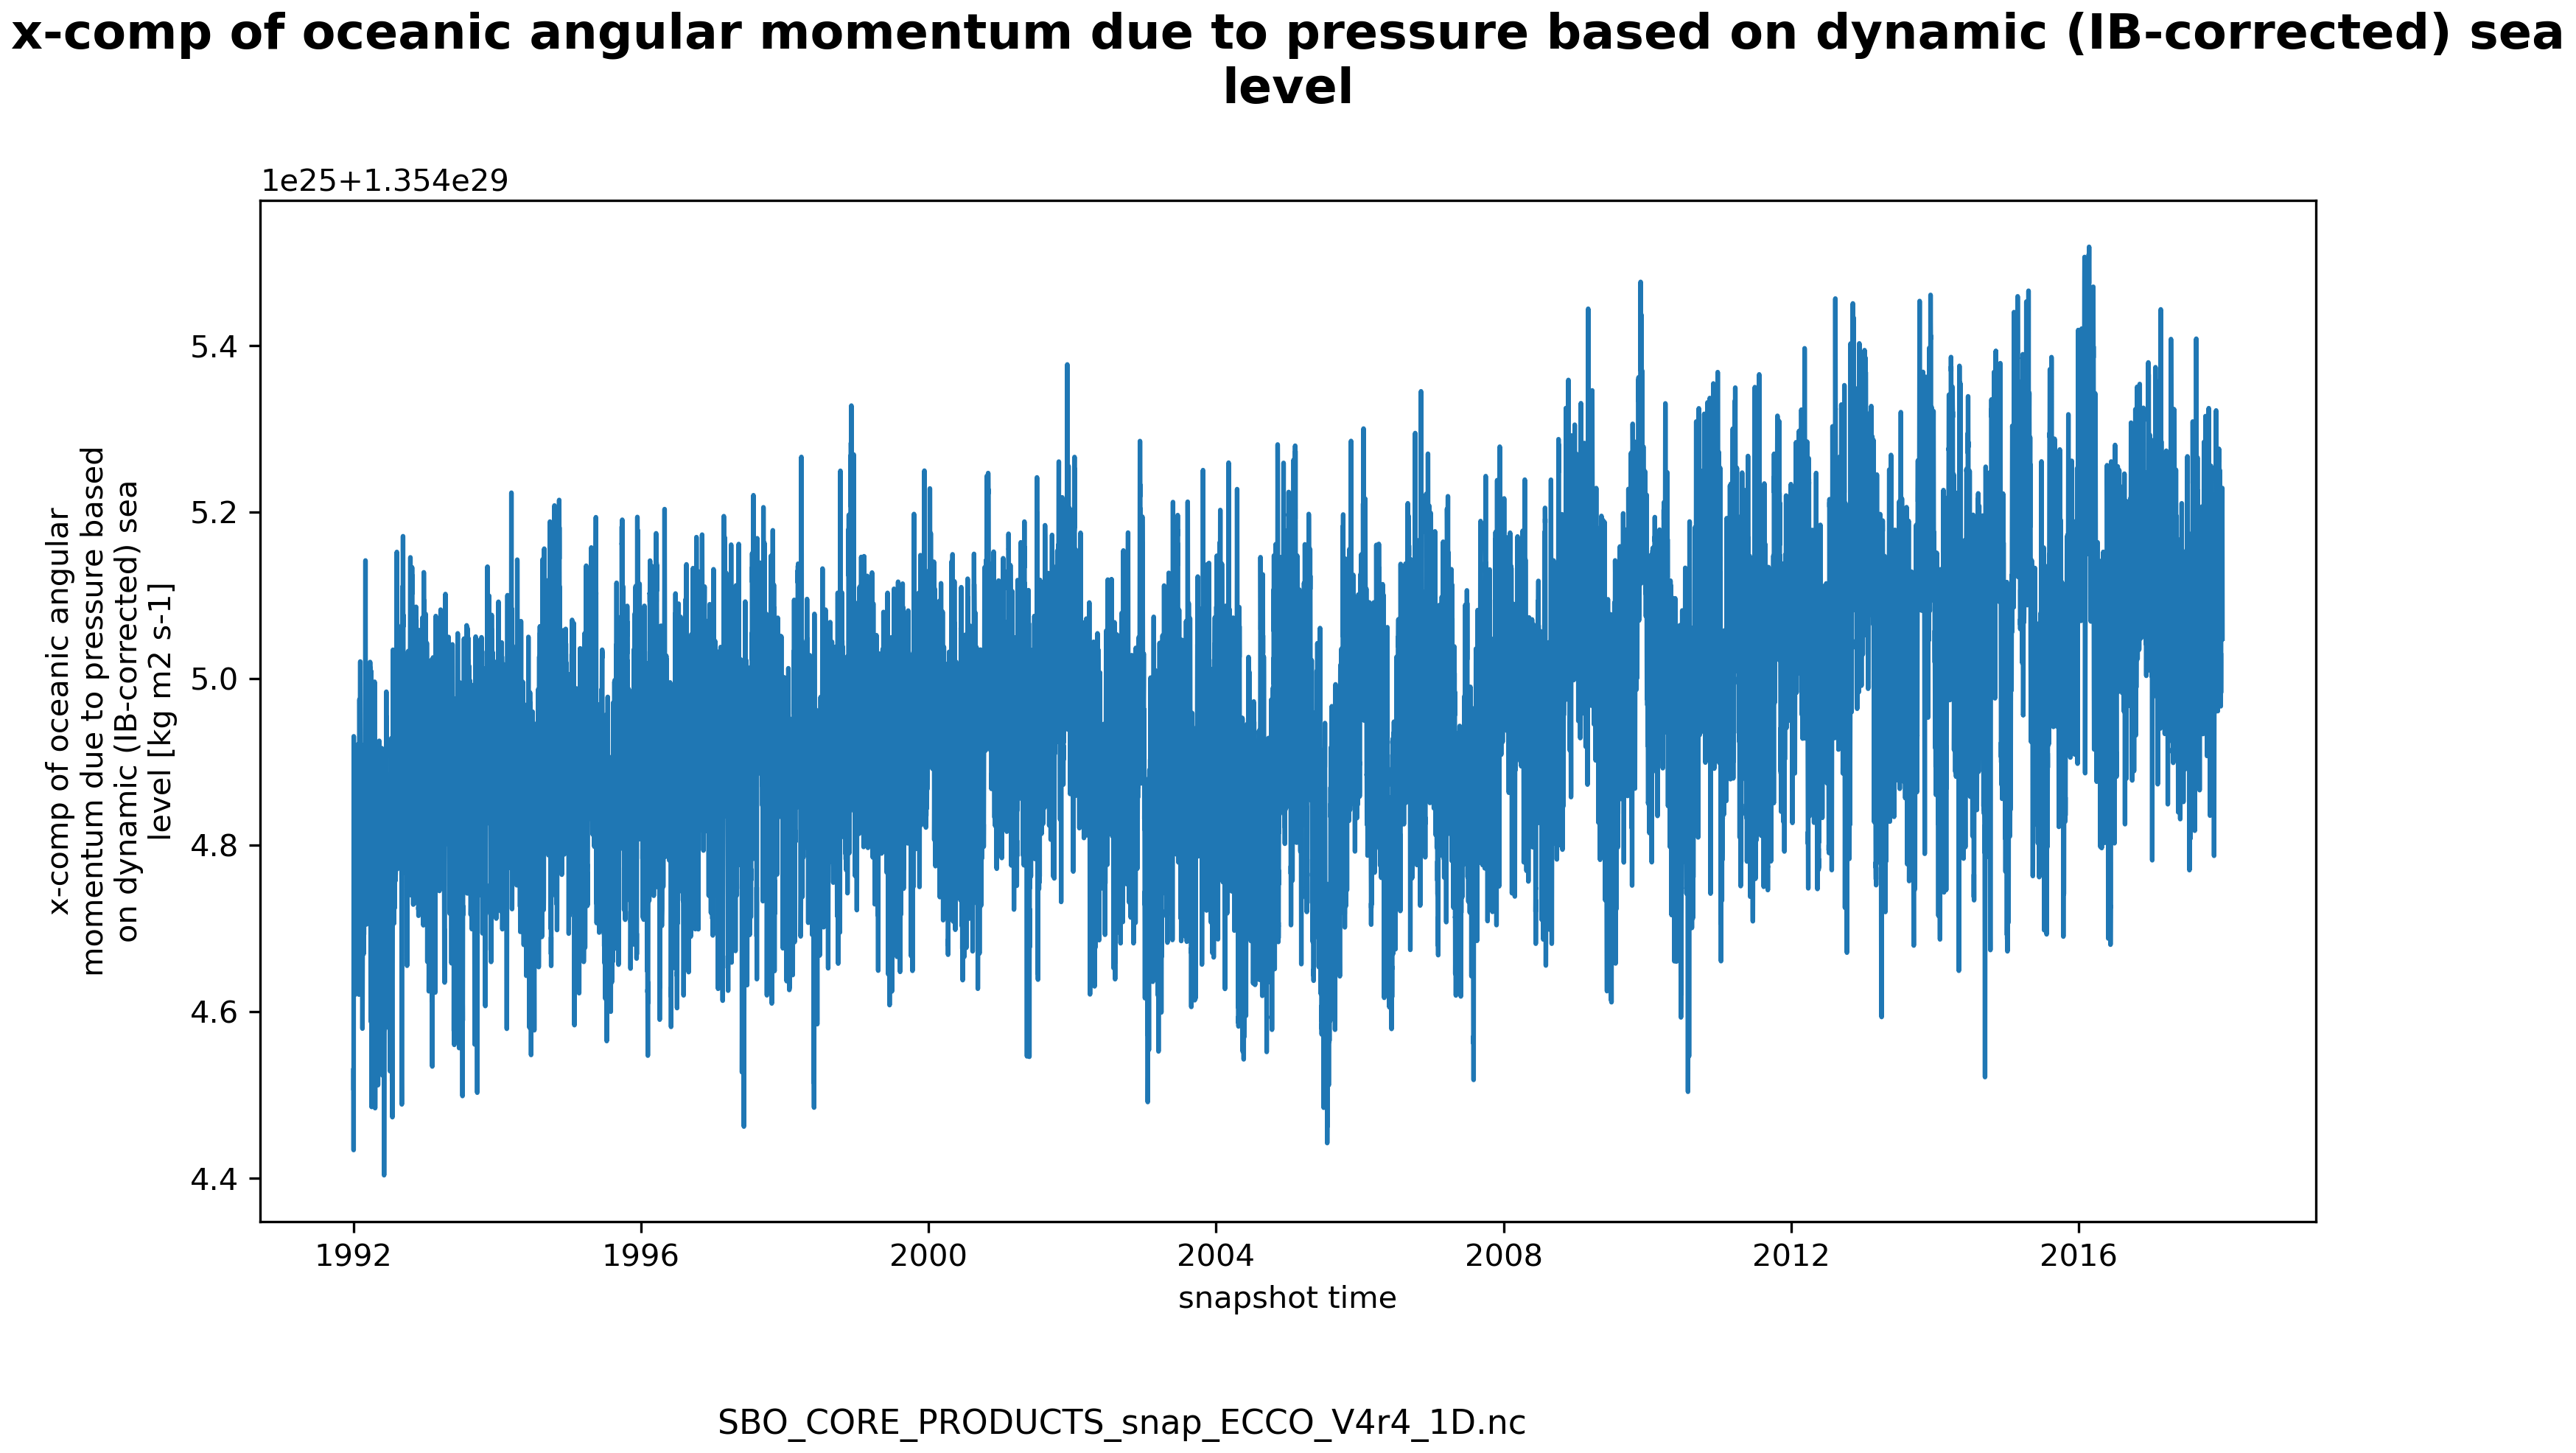
\includegraphics[scale=0.55]{../images/plots/v4r4/oneD_plots/SBO_Core_Products/xoamp_dsl.png}
\caption{Dataset: SBO\_CORE\_PRODUCTS, Variable: xoamp\_dsl}
\label{tab:table-SBO_CORE_PRODUCTS_xoamp_dsl-Plot}
\end{figure}
\newpage
\pagebreak
\subsubsection{1D Variable: xoamp\_fw}
\begin{longtable}{|m{0.06\textwidth}|m{0.3\textwidth}|m{0.45\textwidth}|m{0.12\textwidth}|}
\caption{Attributes description of the variable 'xoamp\_fw' from SBO\_CORE\_PRODUCTS's  dataset.}
\label{tab:table-SBO_CORE_PRODUCTS_xoamp_fw} \\ 
\hline \endhead \hline \endfoot
\rowcolor{lightgray} \textbf{Storage Type} & \textbf{Variable Name} & \textbf{Description} & \textbf{Unit} \\ \hline
float64 & xoamp\_fw & X-comp of oceanic angular momentum due to freshwater flux & kg m2 s-1 \\ \hline
\multicolumn{4}{|c|}{\cellcolor{lightgray}{\textbf{Description of the variable in Common Data language (CDL)}}} \\ \hline
\multicolumn{4}{|c|}{\fontfamily{lmtt}\selectfont{\makecell{\parbox{.95\textwidth}{\vspace*{0.25cm} \footnotesize{float64 xoamp\_fw(time)\\
\hspace*{0.5cm}xoamp\_fw: \_FillValue = 9.969209968386869e+36\\
\hspace*{0.5cm}xoamp\_fw: coordinates = time\\
\hspace*{0.5cm}xoamp\_fw: coverage\_content\_type = modelResult\\
\hspace*{0.5cm}xoamp\_fw: long\_name = x-comp of oceanic angular momentum due to freshwater flux\\
\hspace*{0.5cm}xoamp\_fw: units = kg m2 s-1\\
\hspace*{0.5cm}xoamp\_fw: valid\_max = 3.351358892803656e+24\\
\hspace*{0.5cm}xoamp\_fw: valid\_min = 1.805799644912138e+24\\
}}}}} \\ \hline
\rowcolor{lightgray} \multicolumn{4}{|c|}{\textbf{Comments}} \\ \hline
\multicolumn{4}{|p{1\textwidth}|}{\footnotesize{{N/a}}} \\ \hline
\end{longtable}

\begin{figure}[H]
\centering
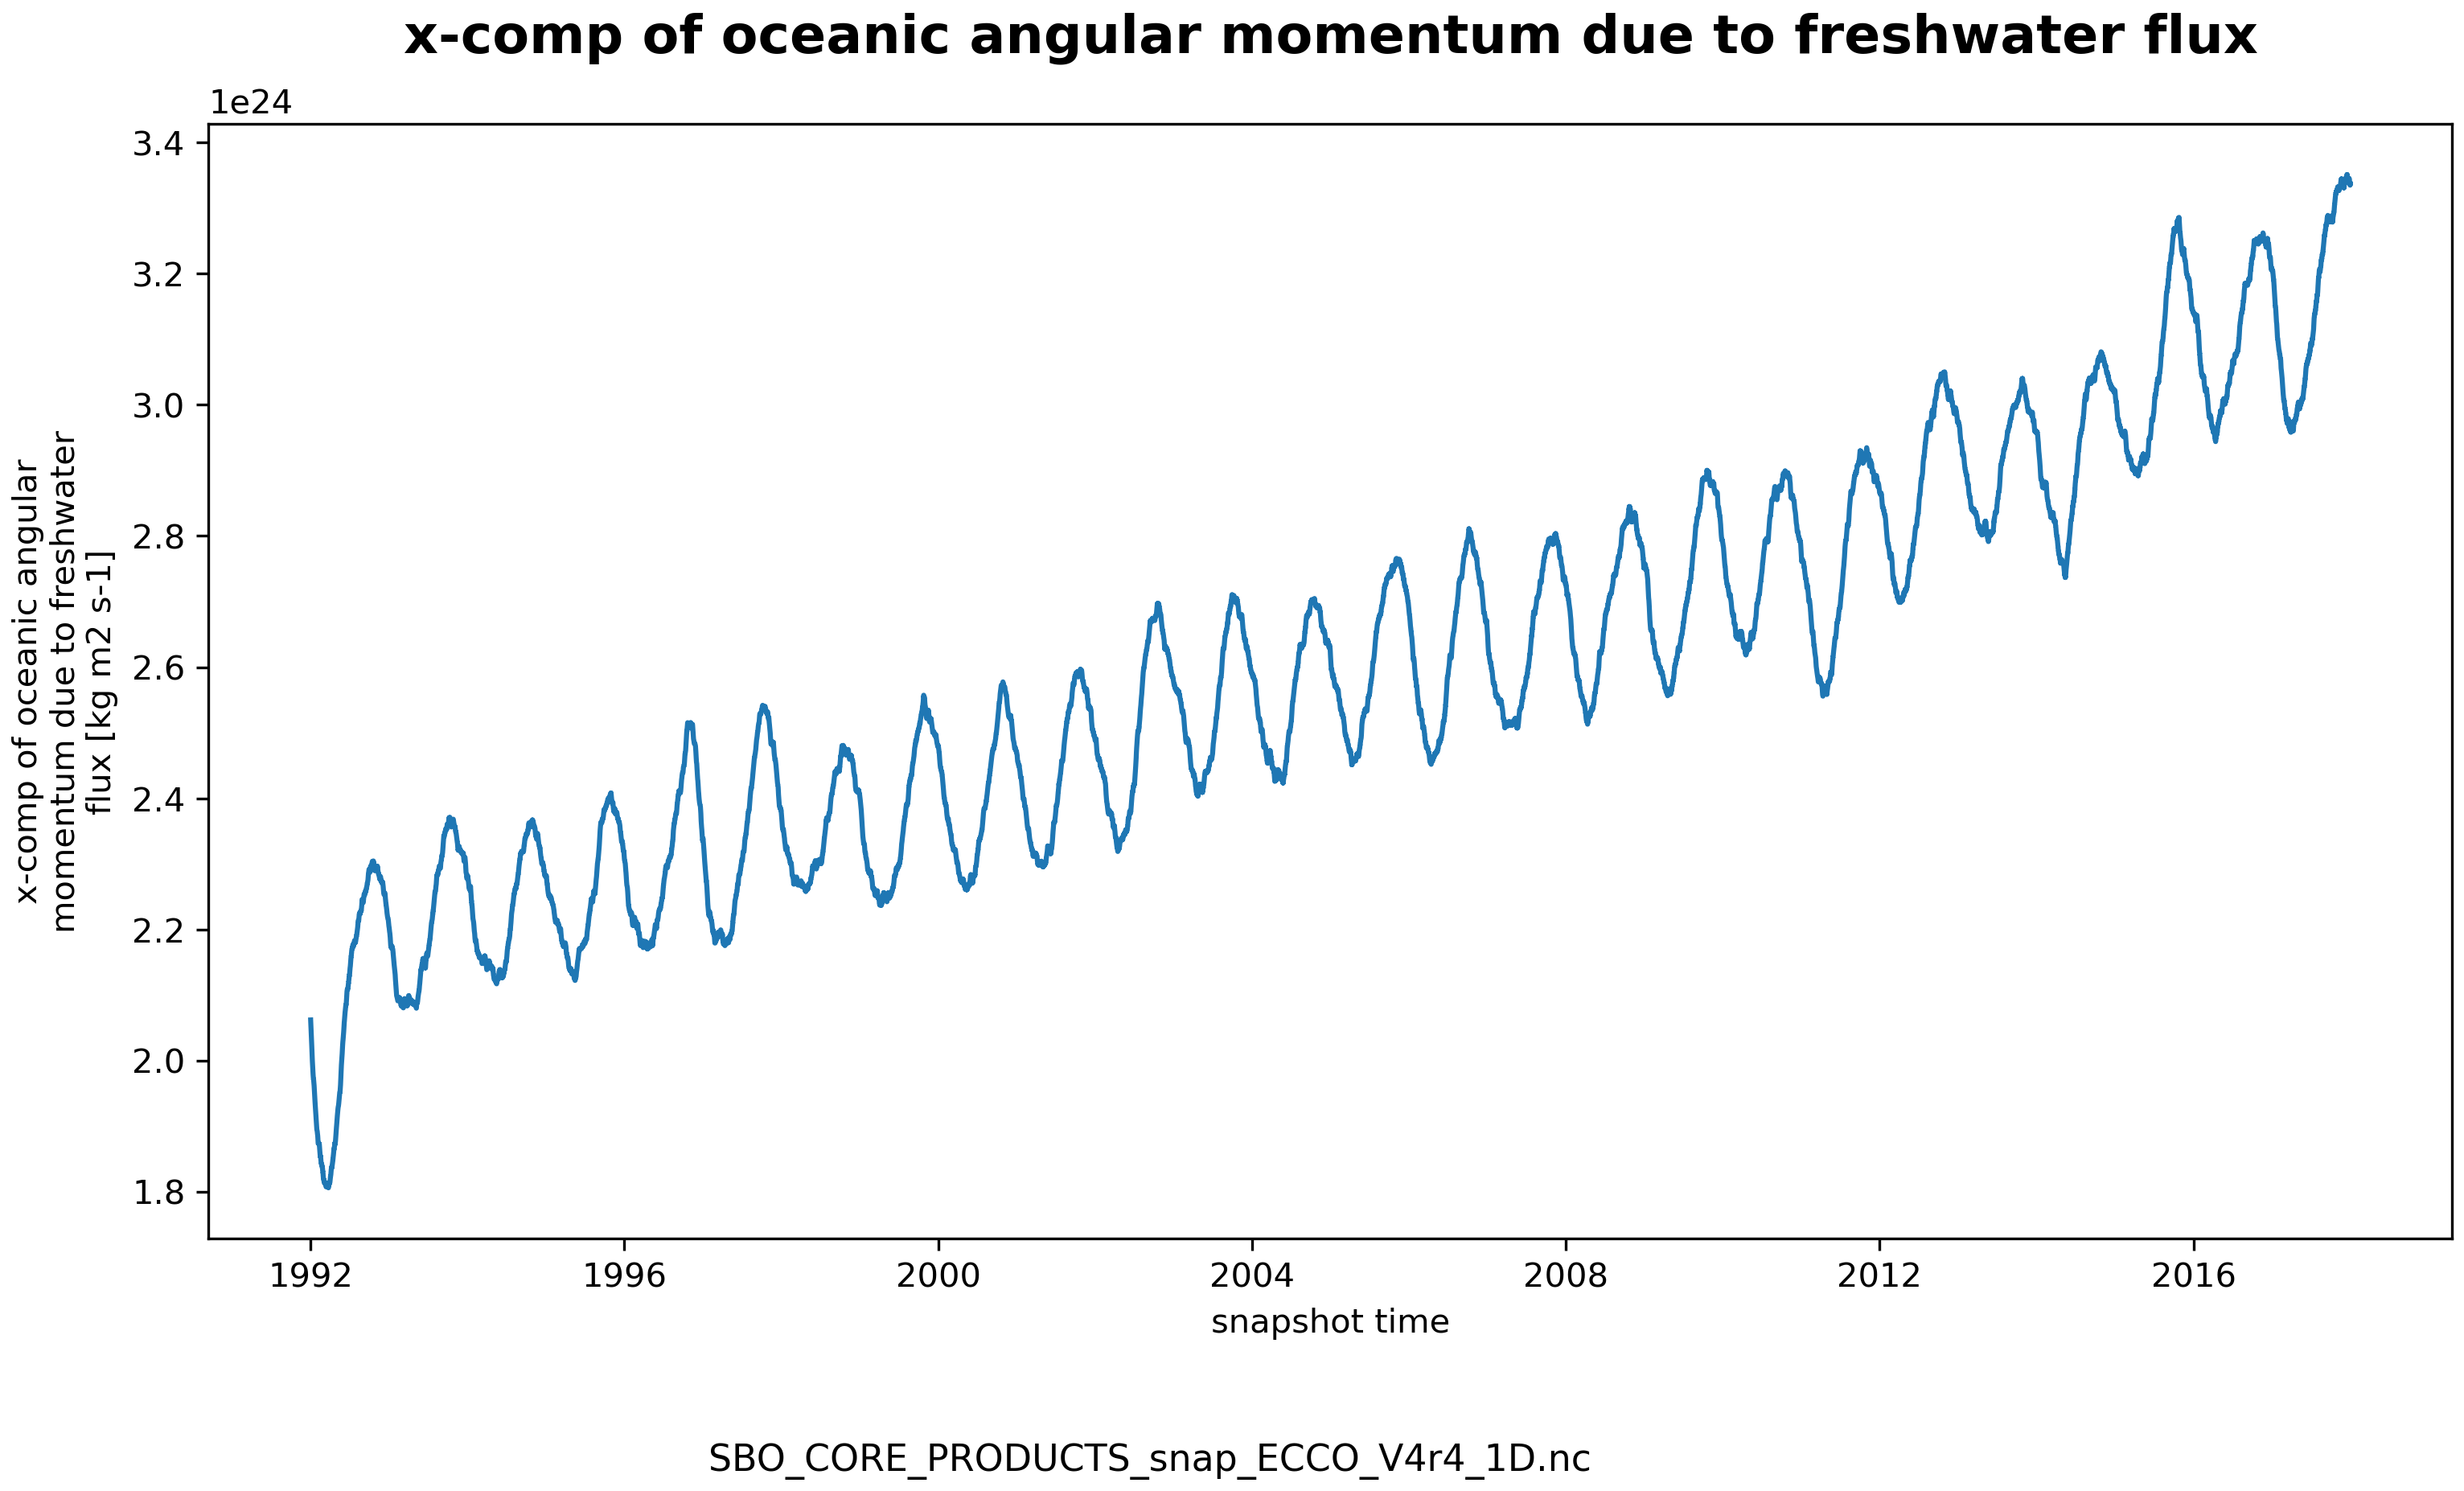
\includegraphics[scale=0.55]{../images/plots/v4r4/oneD_plots/SBO_Core_Products/xoamp_fw.png}
\caption{Dataset: SBO\_CORE\_PRODUCTS, Variable: xoamp\_fw}
\label{tab:table-SBO_CORE_PRODUCTS_xoamp_fw-Plot}
\end{figure}
\newpage
\pagebreak
\subsubsection{1D Variable: ycom}
\begin{longtable}{|m{0.06\textwidth}|m{0.3\textwidth}|m{0.45\textwidth}|m{0.12\textwidth}|}
\caption{Attributes description of the variable 'ycom' from SBO\_CORE\_PRODUCTS's  dataset.}
\label{tab:table-SBO_CORE_PRODUCTS_ycom} \\ 
\hline \endhead \hline \endfoot
\rowcolor{lightgray} \textbf{Storage Type} & \textbf{Variable Name} & \textbf{Description} & \textbf{Unit} \\ \hline
float64 & ycom & Y-comp of center-of-mass of ocean & m \\ \hline
\multicolumn{4}{|c|}{\cellcolor{lightgray}{\textbf{Description of the variable in Common Data language (CDL)}}} \\ \hline
\multicolumn{4}{|c|}{\fontfamily{lmtt}\selectfont{\makecell{\parbox{.95\textwidth}{\vspace*{0.25cm} \footnotesize{float64 ycom(time)\\
\hspace*{0.5cm}ycom: \_FillValue = 9.969209968386869e+36\\
\hspace*{0.5cm}ycom: coordinates = time\\
\hspace*{0.5cm}ycom: coverage\_content\_type = modelResult\\
\hspace*{0.5cm}ycom: long\_name = y-comp of center-of-mass of ocean\\
\hspace*{0.5cm}ycom: units = m\\
\hspace*{0.5cm}ycom: valid\_max = -466327.21844756586\\
\hspace*{0.5cm}ycom: valid\_min = -466387.24450374383\\
}}}}} \\ \hline
\rowcolor{lightgray} \multicolumn{4}{|c|}{\textbf{Comments}} \\ \hline
\multicolumn{4}{|p{1\textwidth}|}{\footnotesize{{N/a}}} \\ \hline
\end{longtable}

\begin{figure}[H]
\centering
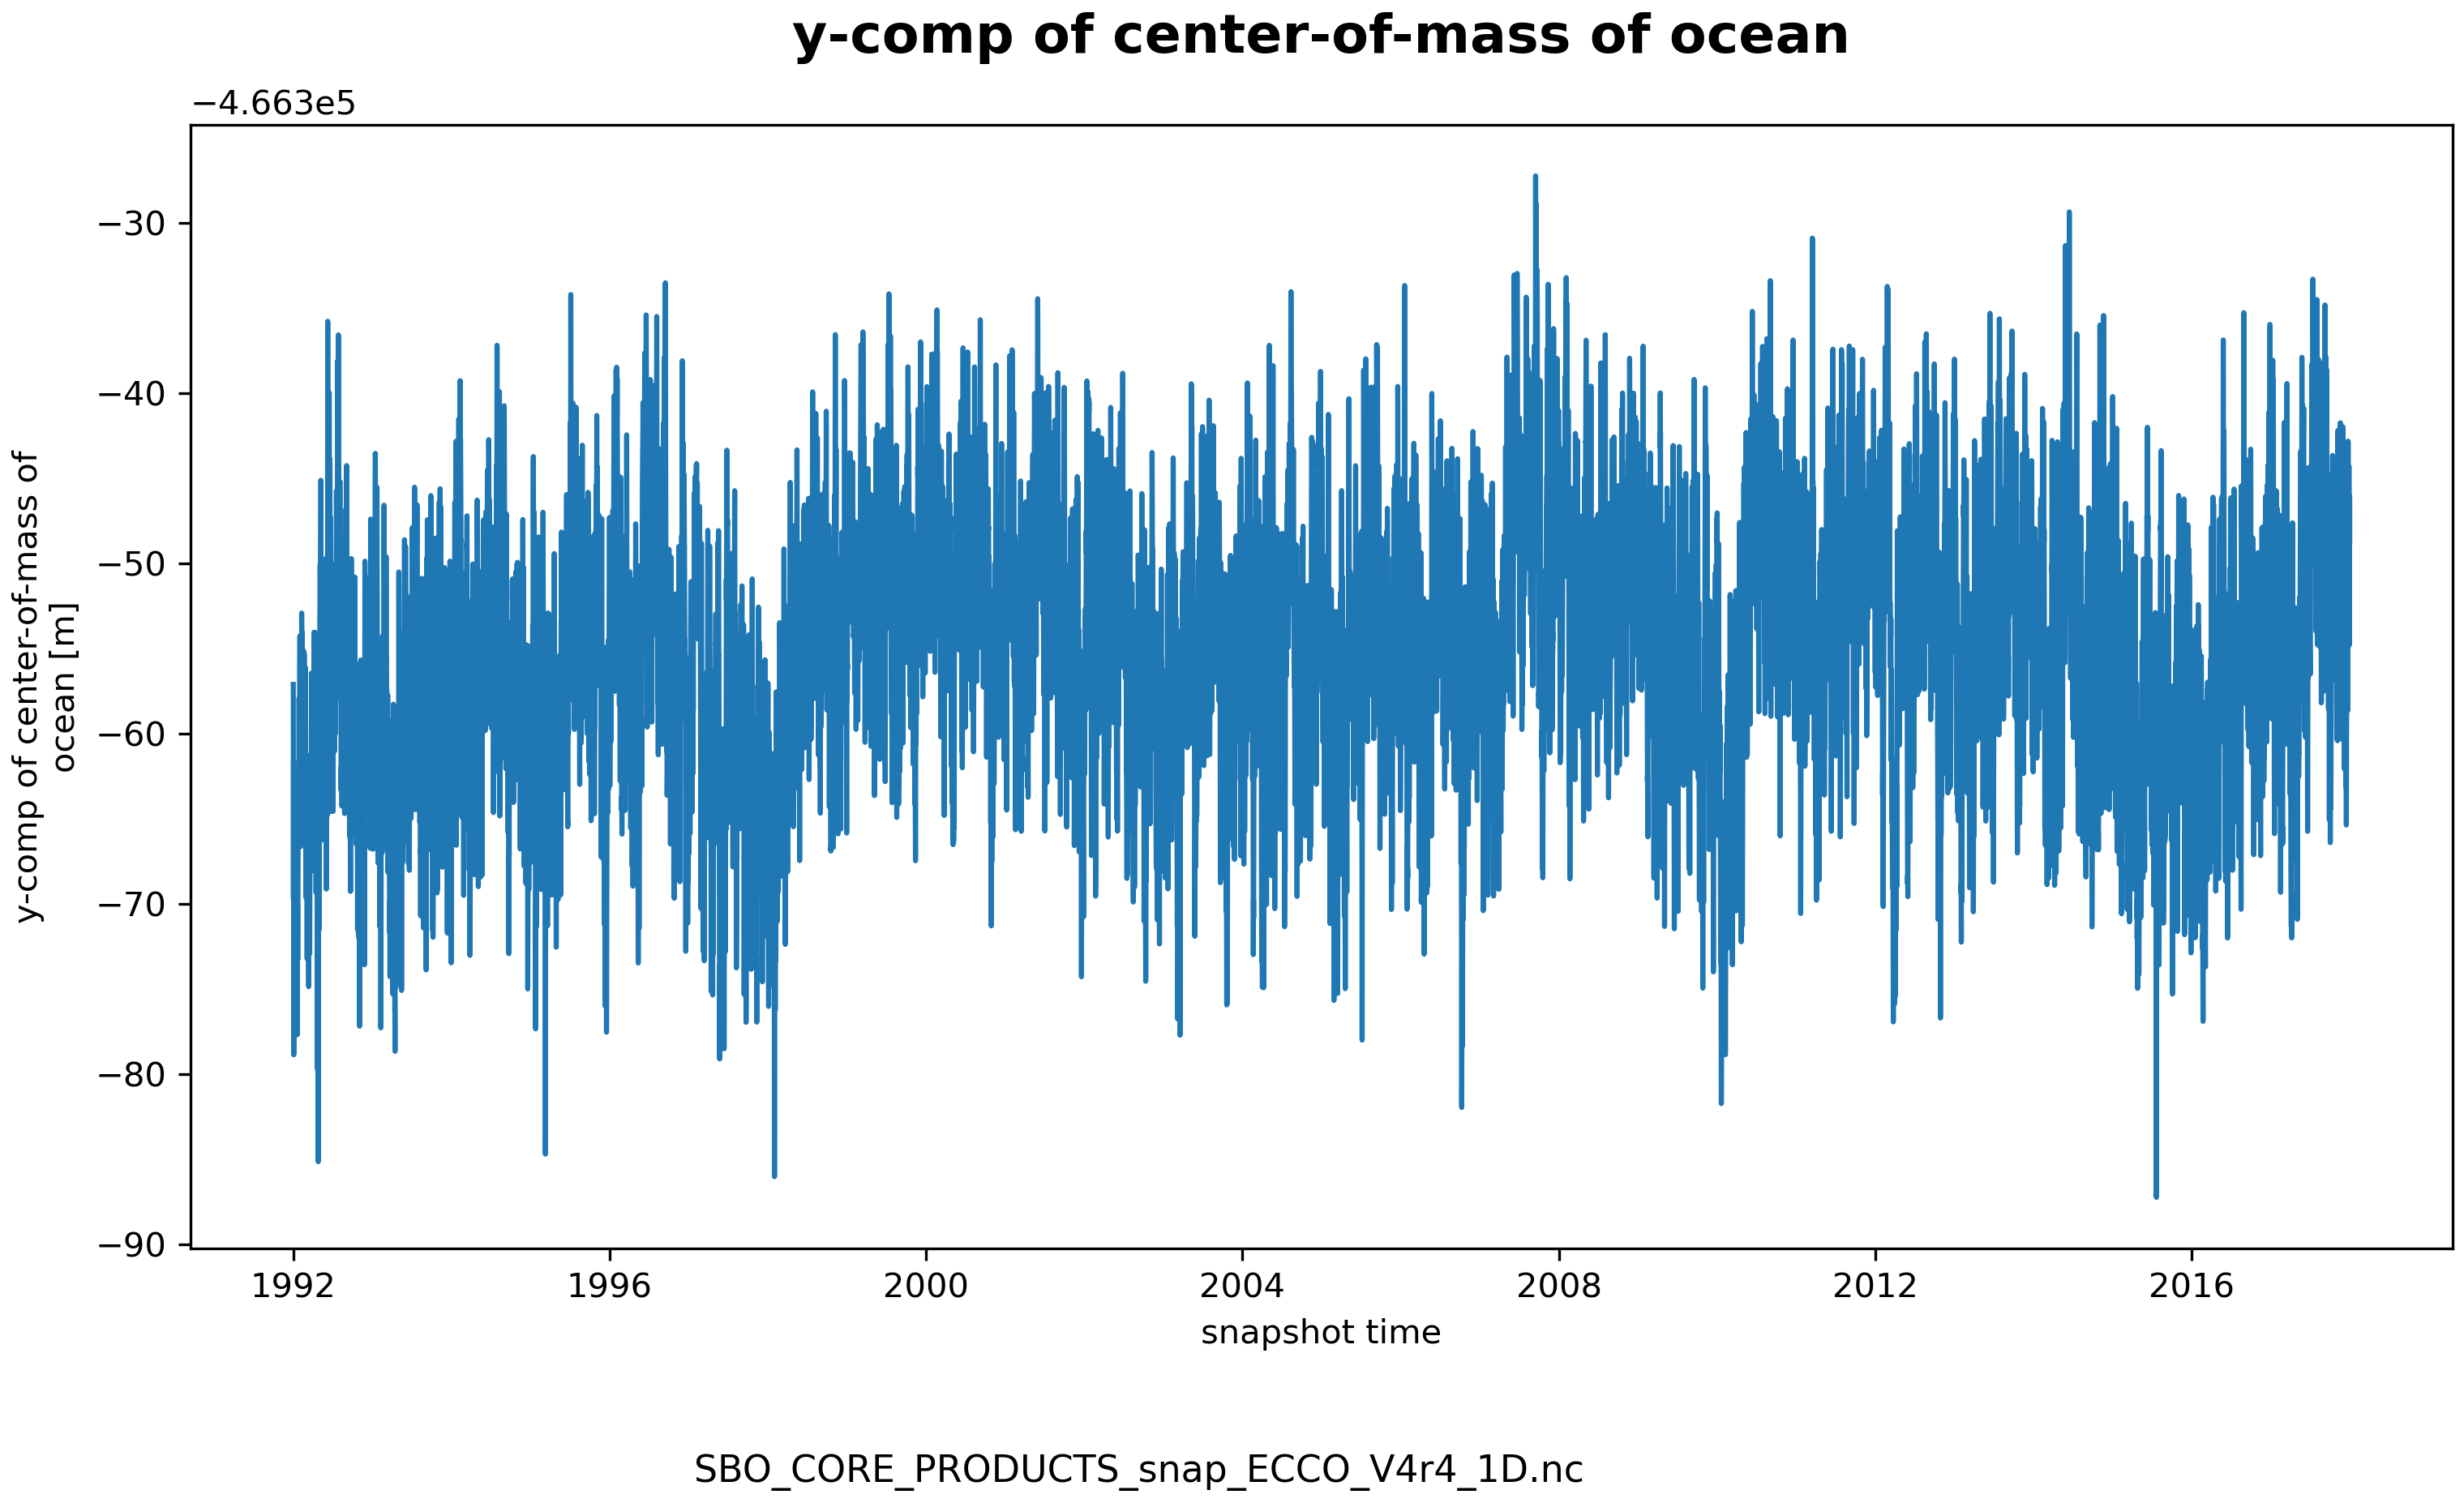
\includegraphics[scale=0.55]{../images/plots/v4r4/oneD_plots/SBO_Core_Products/ycom.png}
\caption{Dataset: SBO\_CORE\_PRODUCTS, Variable: ycom}
\label{tab:table-SBO_CORE_PRODUCTS_ycom-Plot}
\end{figure}
\newpage
\pagebreak
\subsubsection{1D Variable: ycom\_fw}
\begin{longtable}{|m{0.06\textwidth}|m{0.3\textwidth}|m{0.45\textwidth}|m{0.12\textwidth}|}
\caption{Attributes description of the variable 'ycom\_fw' from SBO\_CORE\_PRODUCTS's  dataset.}
\label{tab:table-SBO_CORE_PRODUCTS_ycom_fw} \\ 
\hline \endhead \hline \endfoot
\rowcolor{lightgray} \textbf{Storage Type} & \textbf{Variable Name} & \textbf{Description} & \textbf{Unit} \\ \hline
float64 & ycom\_fw & Y-comp of center-of-mass of freshwater flux & m \\ \hline
\multicolumn{4}{|c|}{\cellcolor{lightgray}{\textbf{Description of the variable in Common Data language (CDL)}}} \\ \hline
\multicolumn{4}{|c|}{\fontfamily{lmtt}\selectfont{\makecell{\parbox{.95\textwidth}{\vspace*{0.25cm} \footnotesize{float64 ycom\_fw(time)\\
\hspace*{0.5cm}ycom\_fw: \_FillValue = 9.969209968386869e+36\\
\hspace*{0.5cm}ycom\_fw: coordinates = time\\
\hspace*{0.5cm}ycom\_fw: coverage\_content\_type = modelResult\\
\hspace*{0.5cm}ycom\_fw: long\_name = y-comp of center-of-mass of freshwater flux\\
\hspace*{0.5cm}ycom\_fw: units = m\\
\hspace*{0.5cm}ycom\_fw: valid\_max = -324750.4152921157\\
\hspace*{0.5cm}ycom\_fw: valid\_min = -324750.41529212013\\
}}}}} \\ \hline
\rowcolor{lightgray} \multicolumn{4}{|c|}{\textbf{Comments}} \\ \hline
\multicolumn{4}{|p{1\textwidth}|}{\footnotesize{{N/a}}} \\ \hline
\end{longtable}

\begin{figure}[H]
\centering
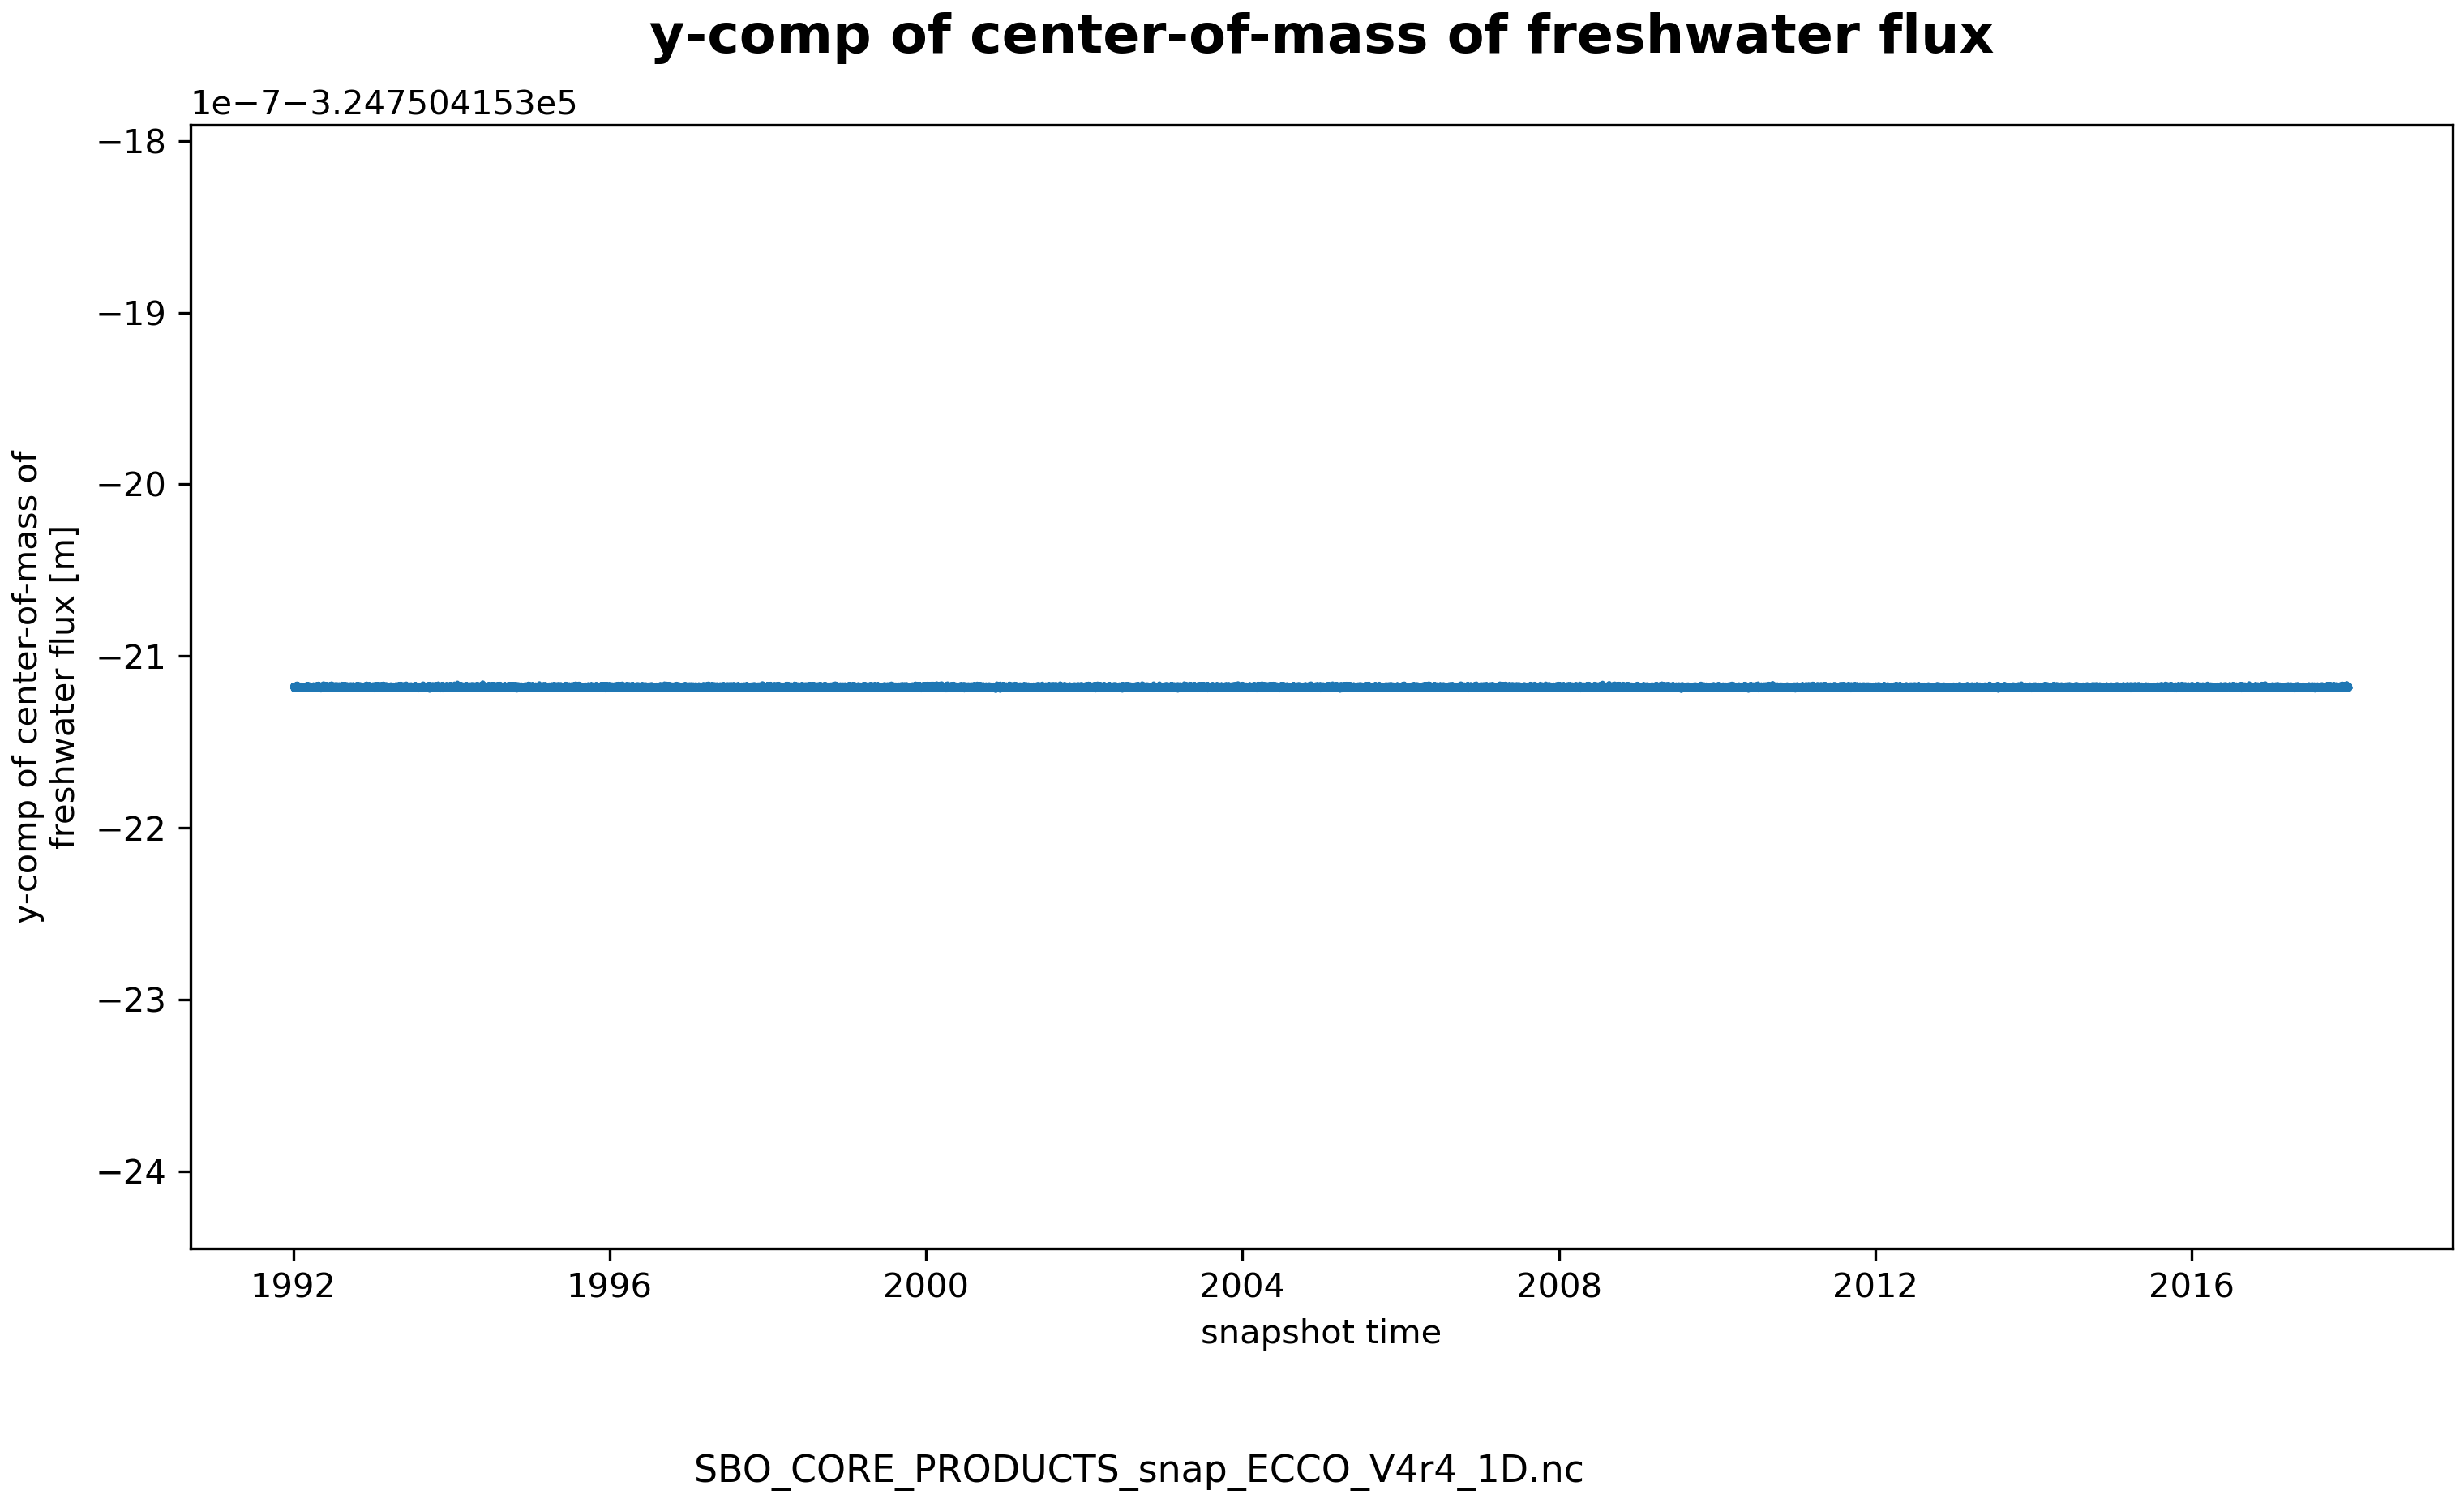
\includegraphics[scale=0.55]{../images/plots/v4r4/oneD_plots/SBO_Core_Products/ycom_fw.png}
\caption{Dataset: SBO\_CORE\_PRODUCTS, Variable: ycom\_fw}
\label{tab:table-SBO_CORE_PRODUCTS_ycom_fw-Plot}
\end{figure}
\newpage
\pagebreak
\subsubsection{1D Variable: yoamc}
\begin{longtable}{|m{0.06\textwidth}|m{0.3\textwidth}|m{0.45\textwidth}|m{0.12\textwidth}|}
\caption{Attributes description of the variable 'yoamc' from SBO\_CORE\_PRODUCTS's  dataset.}
\label{tab:table-SBO_CORE_PRODUCTS_yoamc} \\ 
\hline \endhead \hline \endfoot
\rowcolor{lightgray} \textbf{Storage Type} & \textbf{Variable Name} & \textbf{Description} & \textbf{Unit} \\ \hline
float64 & yoamc & Y-comp of oceanic angular momentum due to currents & kg m2 s-1 \\ \hline
\multicolumn{4}{|c|}{\cellcolor{lightgray}{\textbf{Description of the variable in Common Data language (CDL)}}} \\ \hline
\multicolumn{4}{|c|}{\fontfamily{lmtt}\selectfont{\makecell{\parbox{.95\textwidth}{\vspace*{0.25cm} \footnotesize{float64 yoamc(time)\\
\hspace*{0.5cm}yoamc: \_FillValue = 9.969209968386869e+36\\
\hspace*{0.5cm}yoamc: coordinates = time\\
\hspace*{0.5cm}yoamc: coverage\_content\_type = modelResult\\
\hspace*{0.5cm}yoamc: long\_name = y-comp of oceanic angular momentum due to currents\\
\hspace*{0.5cm}yoamc: units = kg m2 s-1\\
\hspace*{0.5cm}yoamc: valid\_max = 4.179441018940977e+24\\
\hspace*{0.5cm}yoamc: valid\_min = -2.19249690136359e+24\\
}}}}} \\ \hline
\rowcolor{lightgray} \multicolumn{4}{|c|}{\textbf{Comments}} \\ \hline
\multicolumn{4}{|p{1\textwidth}|}{\footnotesize{{N/a}}} \\ \hline
\end{longtable}

\begin{figure}[H]
\centering
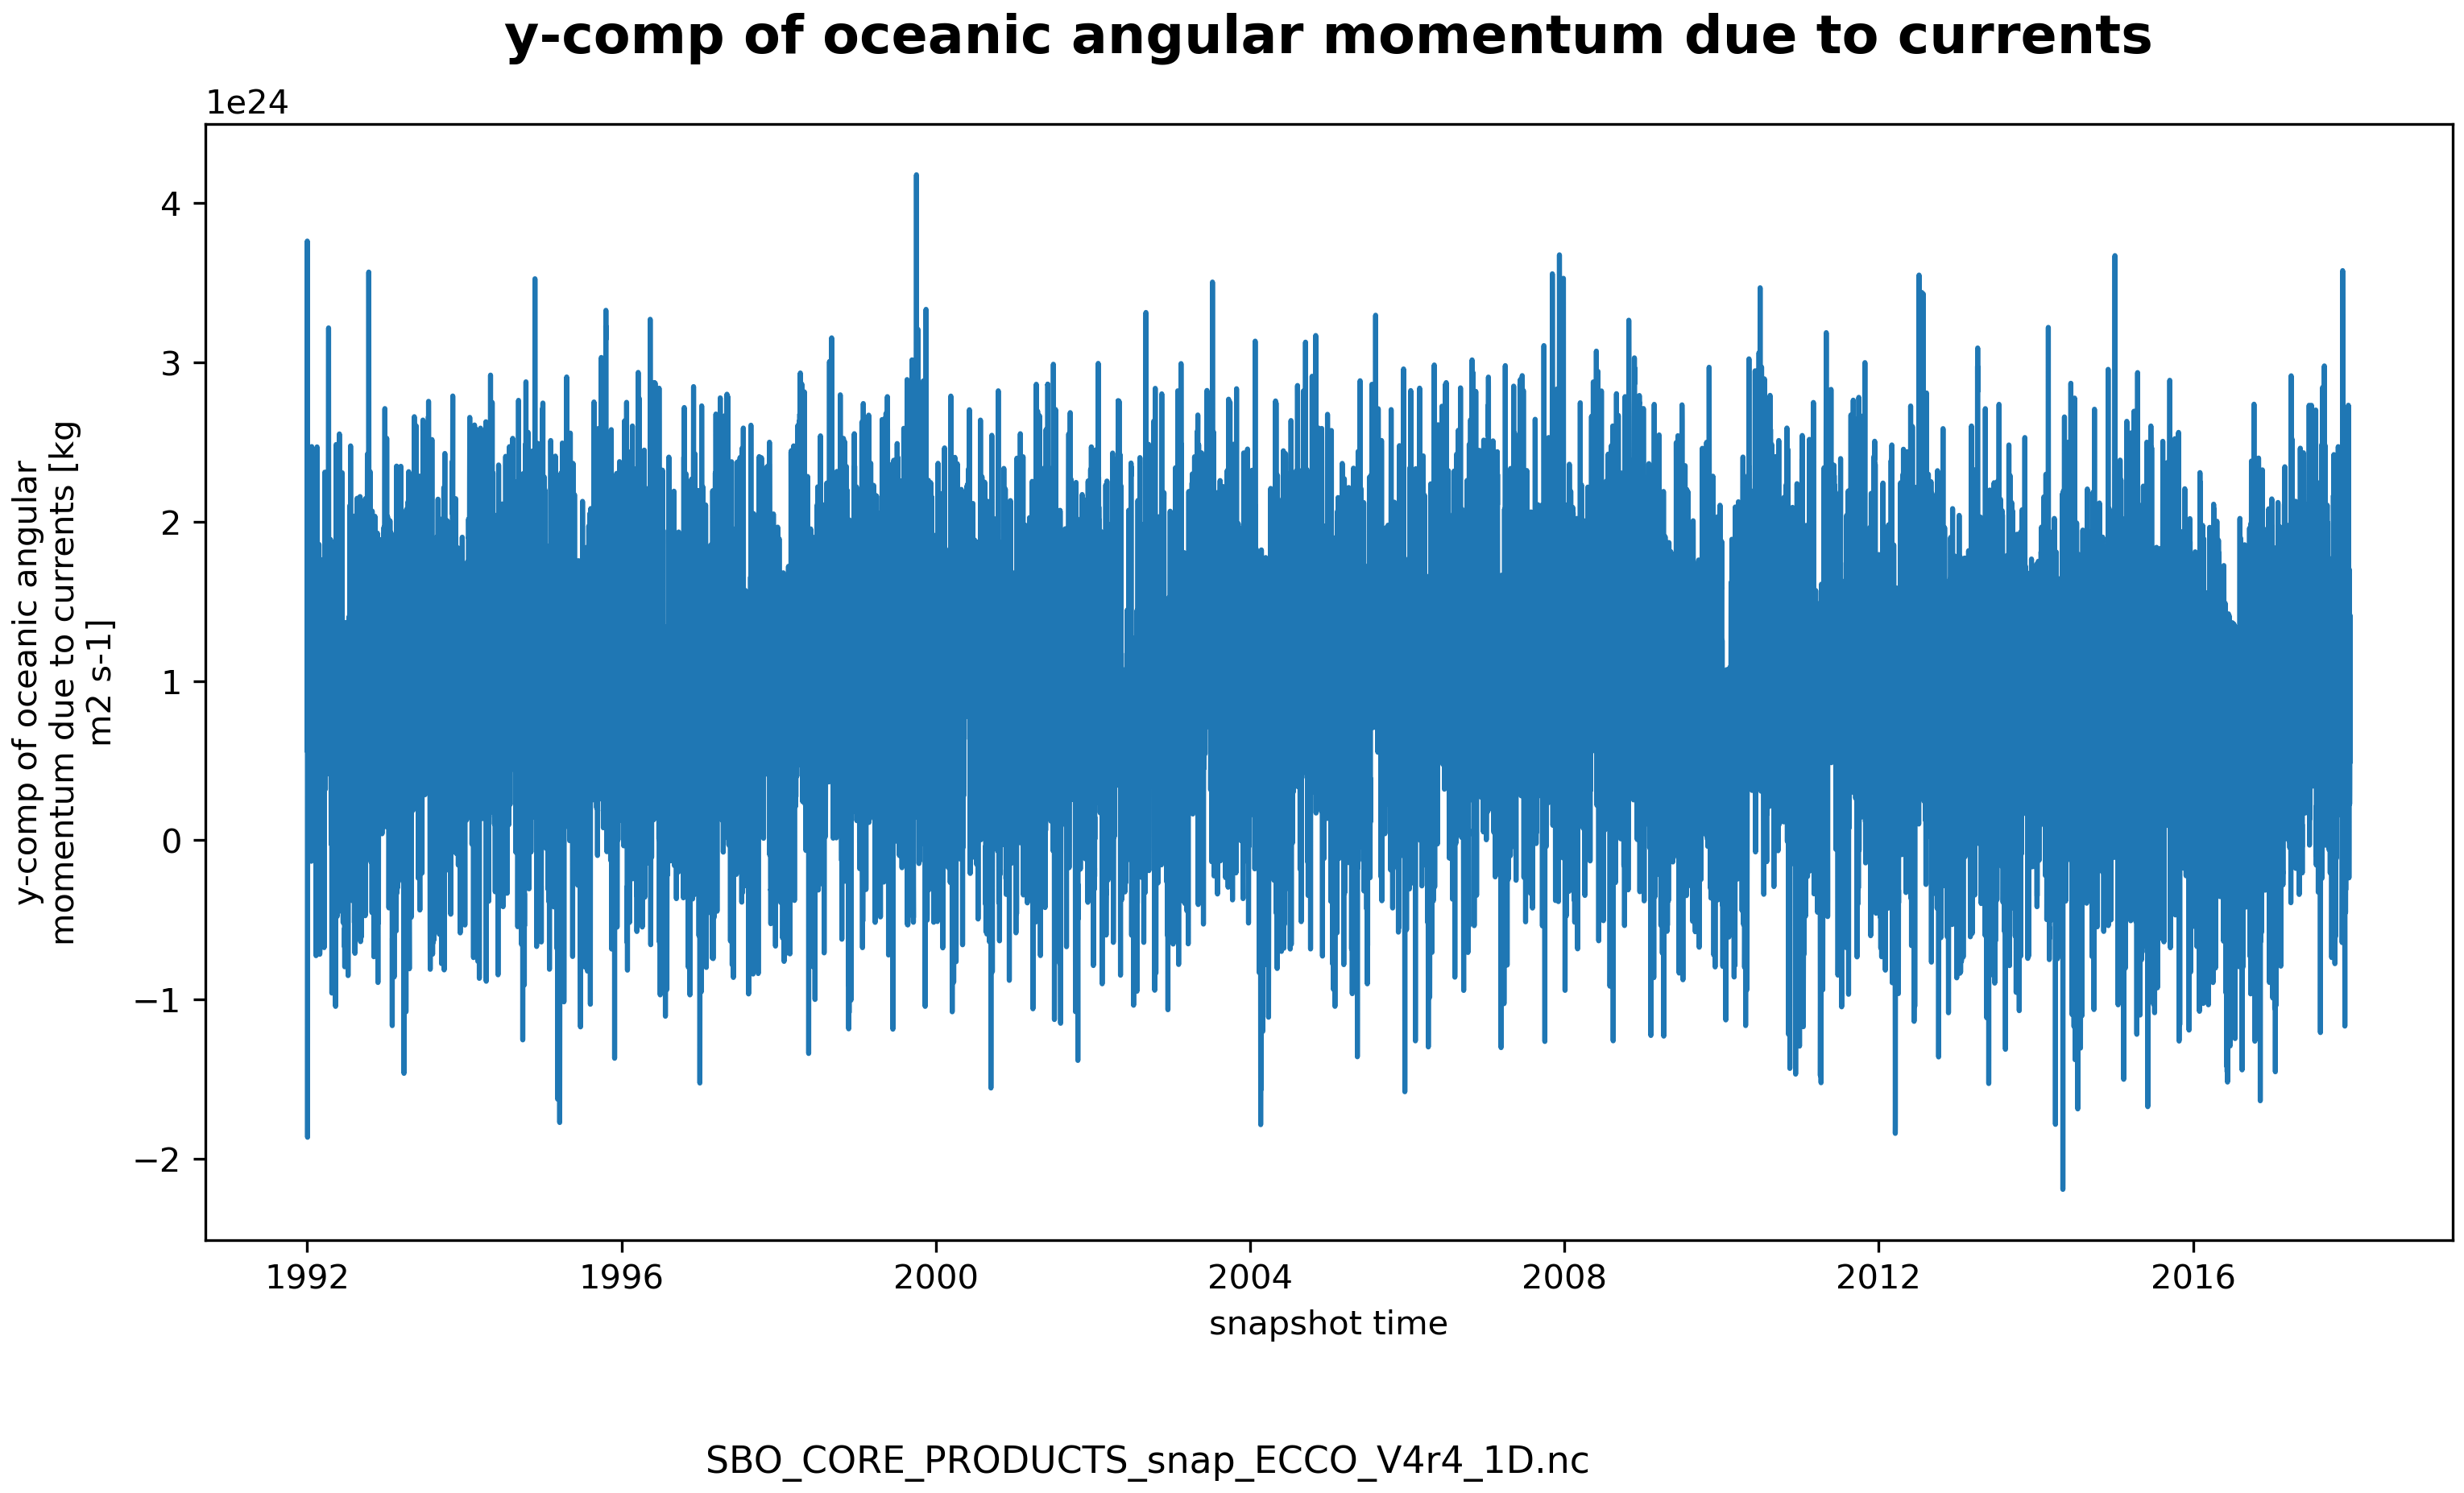
\includegraphics[scale=0.55]{../images/plots/v4r4/oneD_plots/SBO_Core_Products/yoamc.png}
\caption{Dataset: SBO\_CORE\_PRODUCTS, Variable: yoamc}
\label{tab:table-SBO_CORE_PRODUCTS_yoamc-Plot}
\end{figure}
\newpage
\pagebreak
\subsubsection{1D Variable: yoamc\_si}
\begin{longtable}{|m{0.06\textwidth}|m{0.3\textwidth}|m{0.45\textwidth}|m{0.12\textwidth}|}
\caption{Attributes description of the variable 'yoamc\_si' from SBO\_CORE\_PRODUCTS's  dataset.}
\label{tab:table-SBO_CORE_PRODUCTS_yoamc_si} \\ 
\hline \endhead \hline \endfoot
\rowcolor{lightgray} \textbf{Storage Type} & \textbf{Variable Name} & \textbf{Description} & \textbf{Unit} \\ \hline
float64 & yoamc\_si & Y-comp of oceanic angular momentum due to sea-ice motion & kg m2 s-1 \\ \hline
\multicolumn{4}{|c|}{\cellcolor{lightgray}{\textbf{Description of the variable in Common Data language (CDL)}}} \\ \hline
\multicolumn{4}{|c|}{\fontfamily{lmtt}\selectfont{\makecell{\parbox{.95\textwidth}{\vspace*{0.25cm} \footnotesize{float64 yoamc\_si(time)\\
\hspace*{0.5cm}yoamc\_si: \_FillValue = 9.969209968386869e+36\\
\hspace*{0.5cm}yoamc\_si: coordinates = time\\
\hspace*{0.5cm}yoamc\_si: coverage\_content\_type = modelResult\\
\hspace*{0.5cm}yoamc\_si: long\_name = y-comp of oceanic angular momentum due to sea-ice motion\\
\hspace*{0.5cm}yoamc\_si: units = kg m2 s-1\\
\hspace*{0.5cm}yoamc\_si: valid\_max = 1.6107851446370722e+22\\
\hspace*{0.5cm}yoamc\_si: valid\_min = -1.176556337395274e+22\\
}}}}} \\ \hline
\rowcolor{lightgray} \multicolumn{4}{|c|}{\textbf{Comments}} \\ \hline
\multicolumn{4}{|p{1\textwidth}|}{\footnotesize{{N/a}}} \\ \hline
\end{longtable}

\begin{figure}[H]
\centering
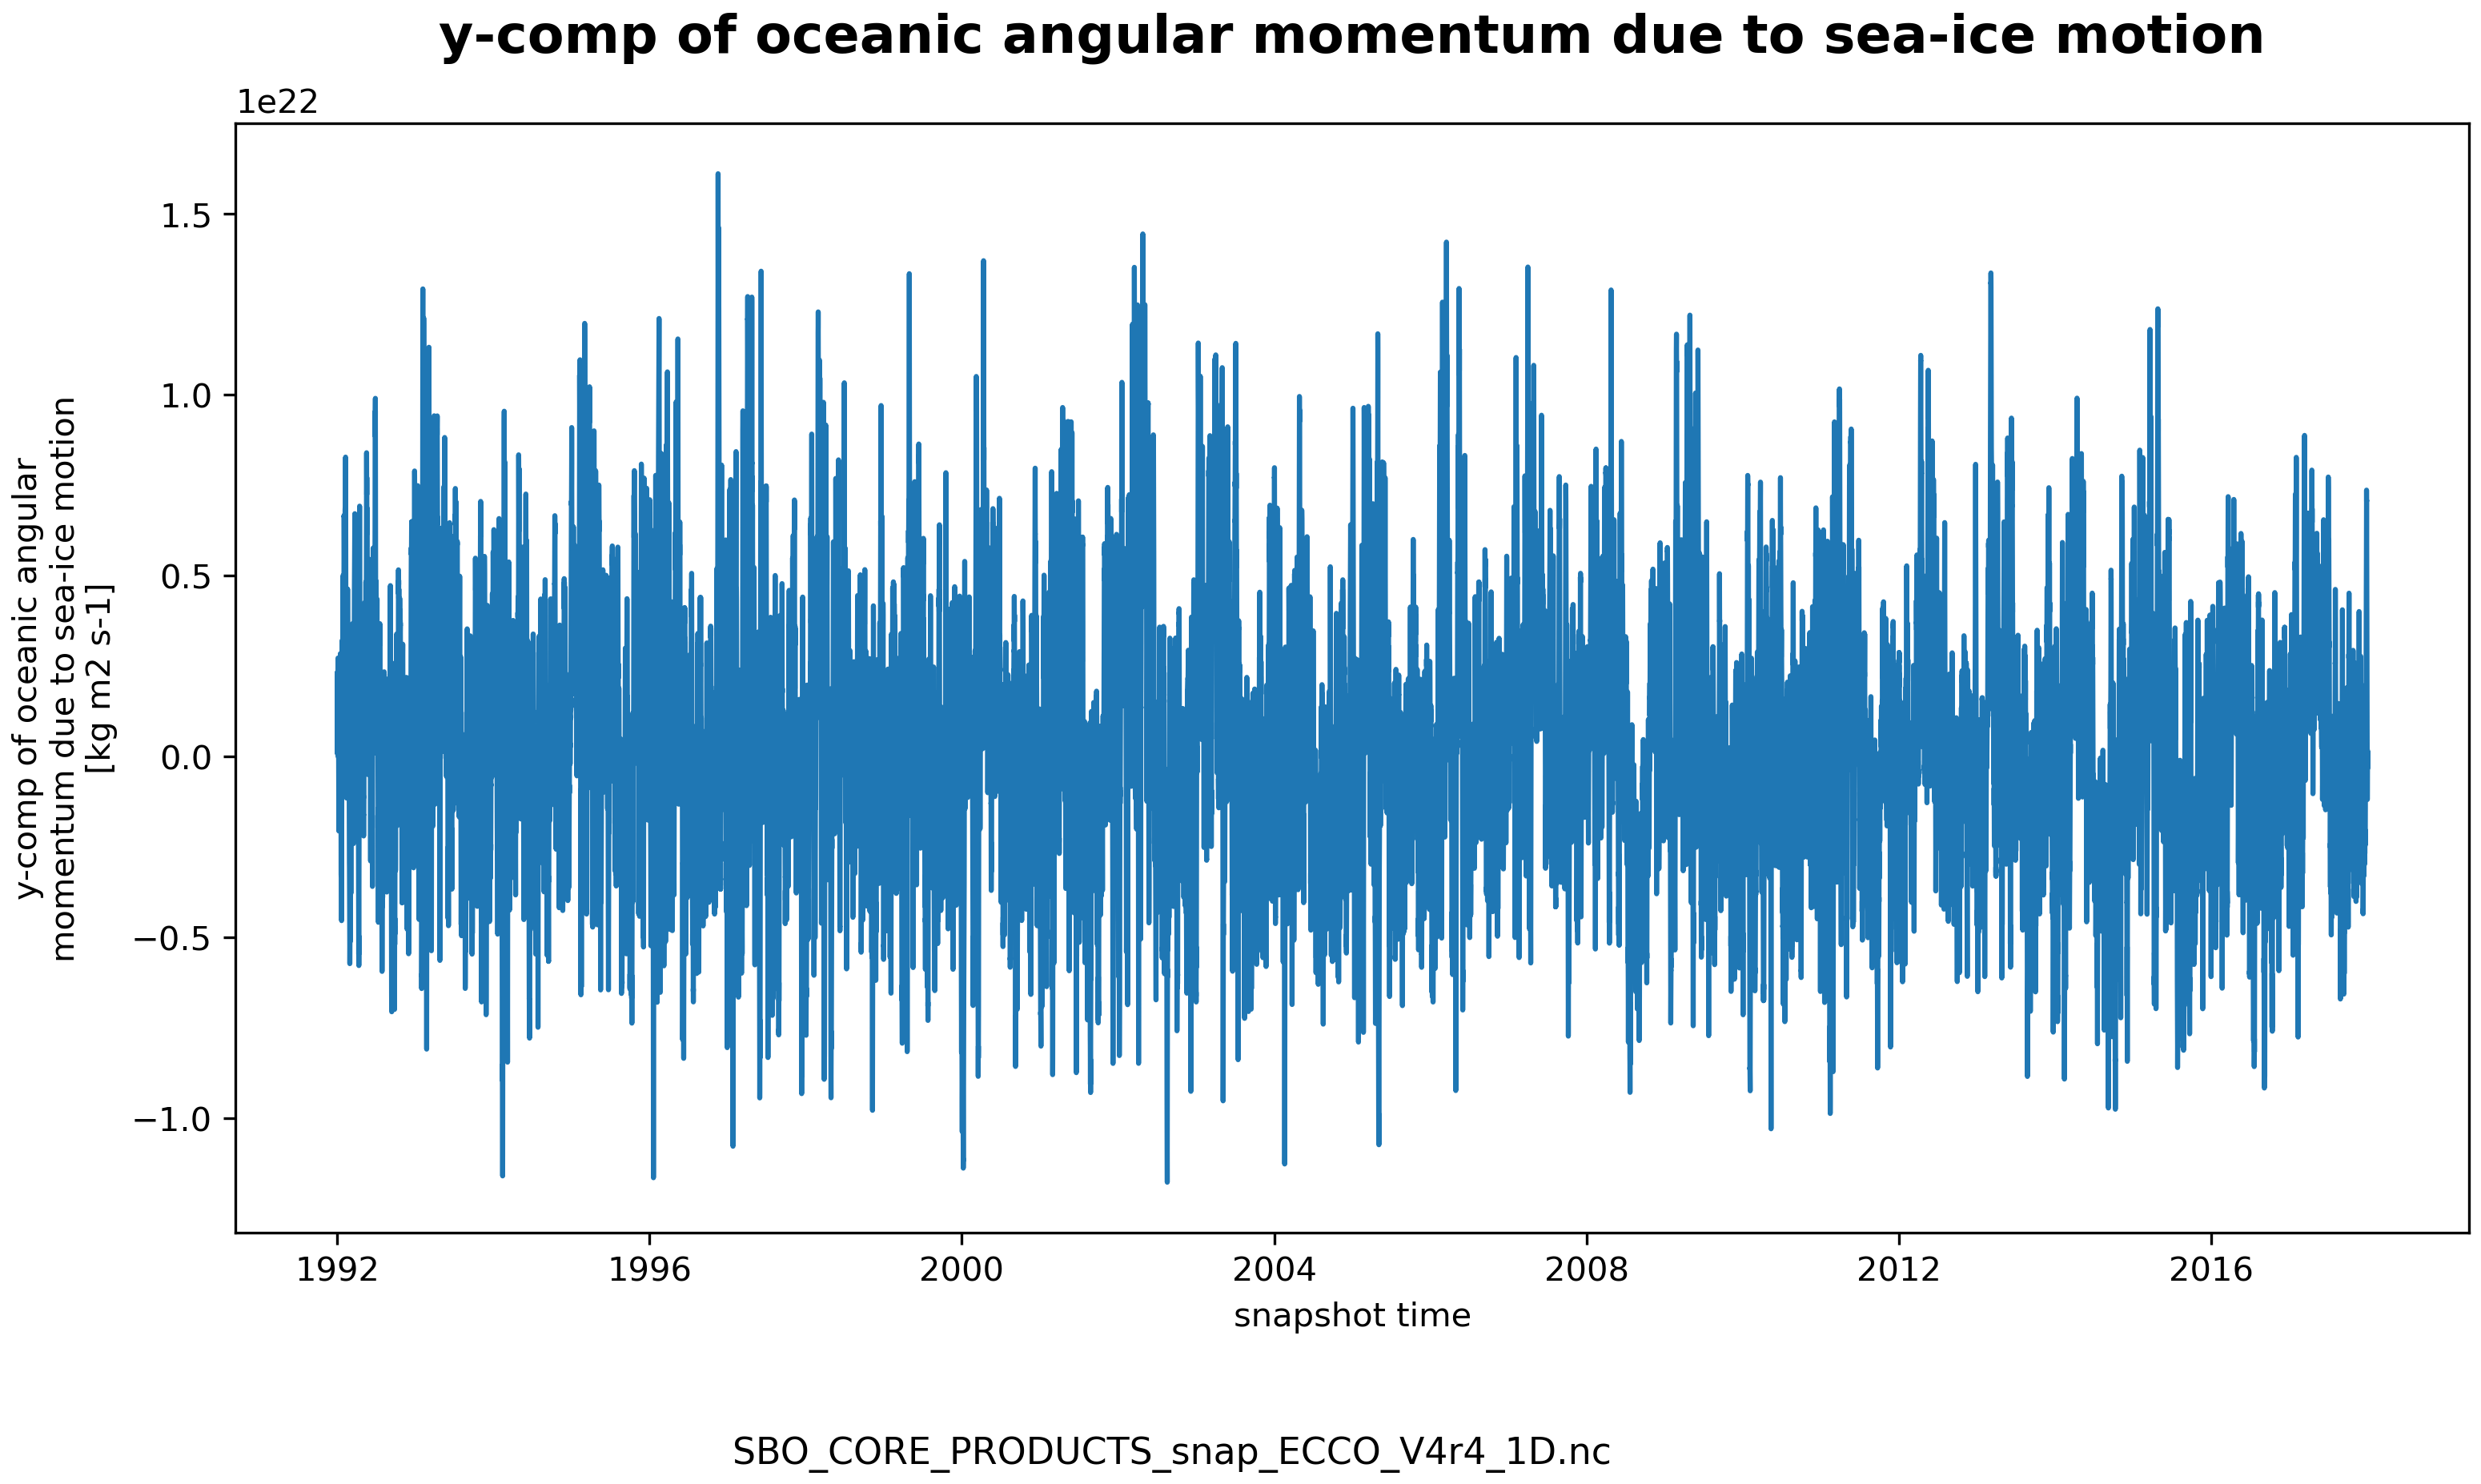
\includegraphics[scale=0.55]{../images/plots/v4r4/oneD_plots/SBO_Core_Products/yoamc_si.png}
\caption{Dataset: SBO\_CORE\_PRODUCTS, Variable: yoamc\_si}
\label{tab:table-SBO_CORE_PRODUCTS_yoamc_si-Plot}
\end{figure}
\newpage
\pagebreak
\subsubsection{1D Variable: yoamp}
\begin{longtable}{|m{0.06\textwidth}|m{0.3\textwidth}|m{0.45\textwidth}|m{0.12\textwidth}|}
\caption{Attributes description of the variable 'yoamp' from SBO\_CORE\_PRODUCTS's  dataset.}
\label{tab:table-SBO_CORE_PRODUCTS_yoamp} \\ 
\hline \endhead \hline \endfoot
\rowcolor{lightgray} \textbf{Storage Type} & \textbf{Variable Name} & \textbf{Description} & \textbf{Unit} \\ \hline
float64 & yoamp & Y-comp of oceanic angular momentum due to pressure & kg m2 s-1 \\ \hline
\multicolumn{4}{|c|}{\cellcolor{lightgray}{\textbf{Description of the variable in Common Data language (CDL)}}} \\ \hline
\multicolumn{4}{|c|}{\fontfamily{lmtt}\selectfont{\makecell{\parbox{.95\textwidth}{\vspace*{0.25cm} \footnotesize{float64 yoamp(time)\\
\hspace*{0.5cm}yoamp: \_FillValue = 9.969209968386869e+36\\
\hspace*{0.5cm}yoamp: coordinates = time\\
\hspace*{0.5cm}yoamp: coverage\_content\_type = modelResult\\
\hspace*{0.5cm}yoamp: long\_name = y-comp of oceanic angular momentum due to pressure\\
\hspace*{0.5cm}yoamp: units = kg m2 s-1\\
\hspace*{0.5cm}yoamp: valid\_max = 1.0478581623131764e+29\\
\hspace*{0.5cm}yoamp: valid\_min = 1.0476388397938864e+29\\
}}}}} \\ \hline
\rowcolor{lightgray} \multicolumn{4}{|c|}{\textbf{Comments}} \\ \hline
\multicolumn{4}{|p{1\textwidth}|}{\footnotesize{{N/a}}} \\ \hline
\end{longtable}

\begin{figure}[H]
\centering
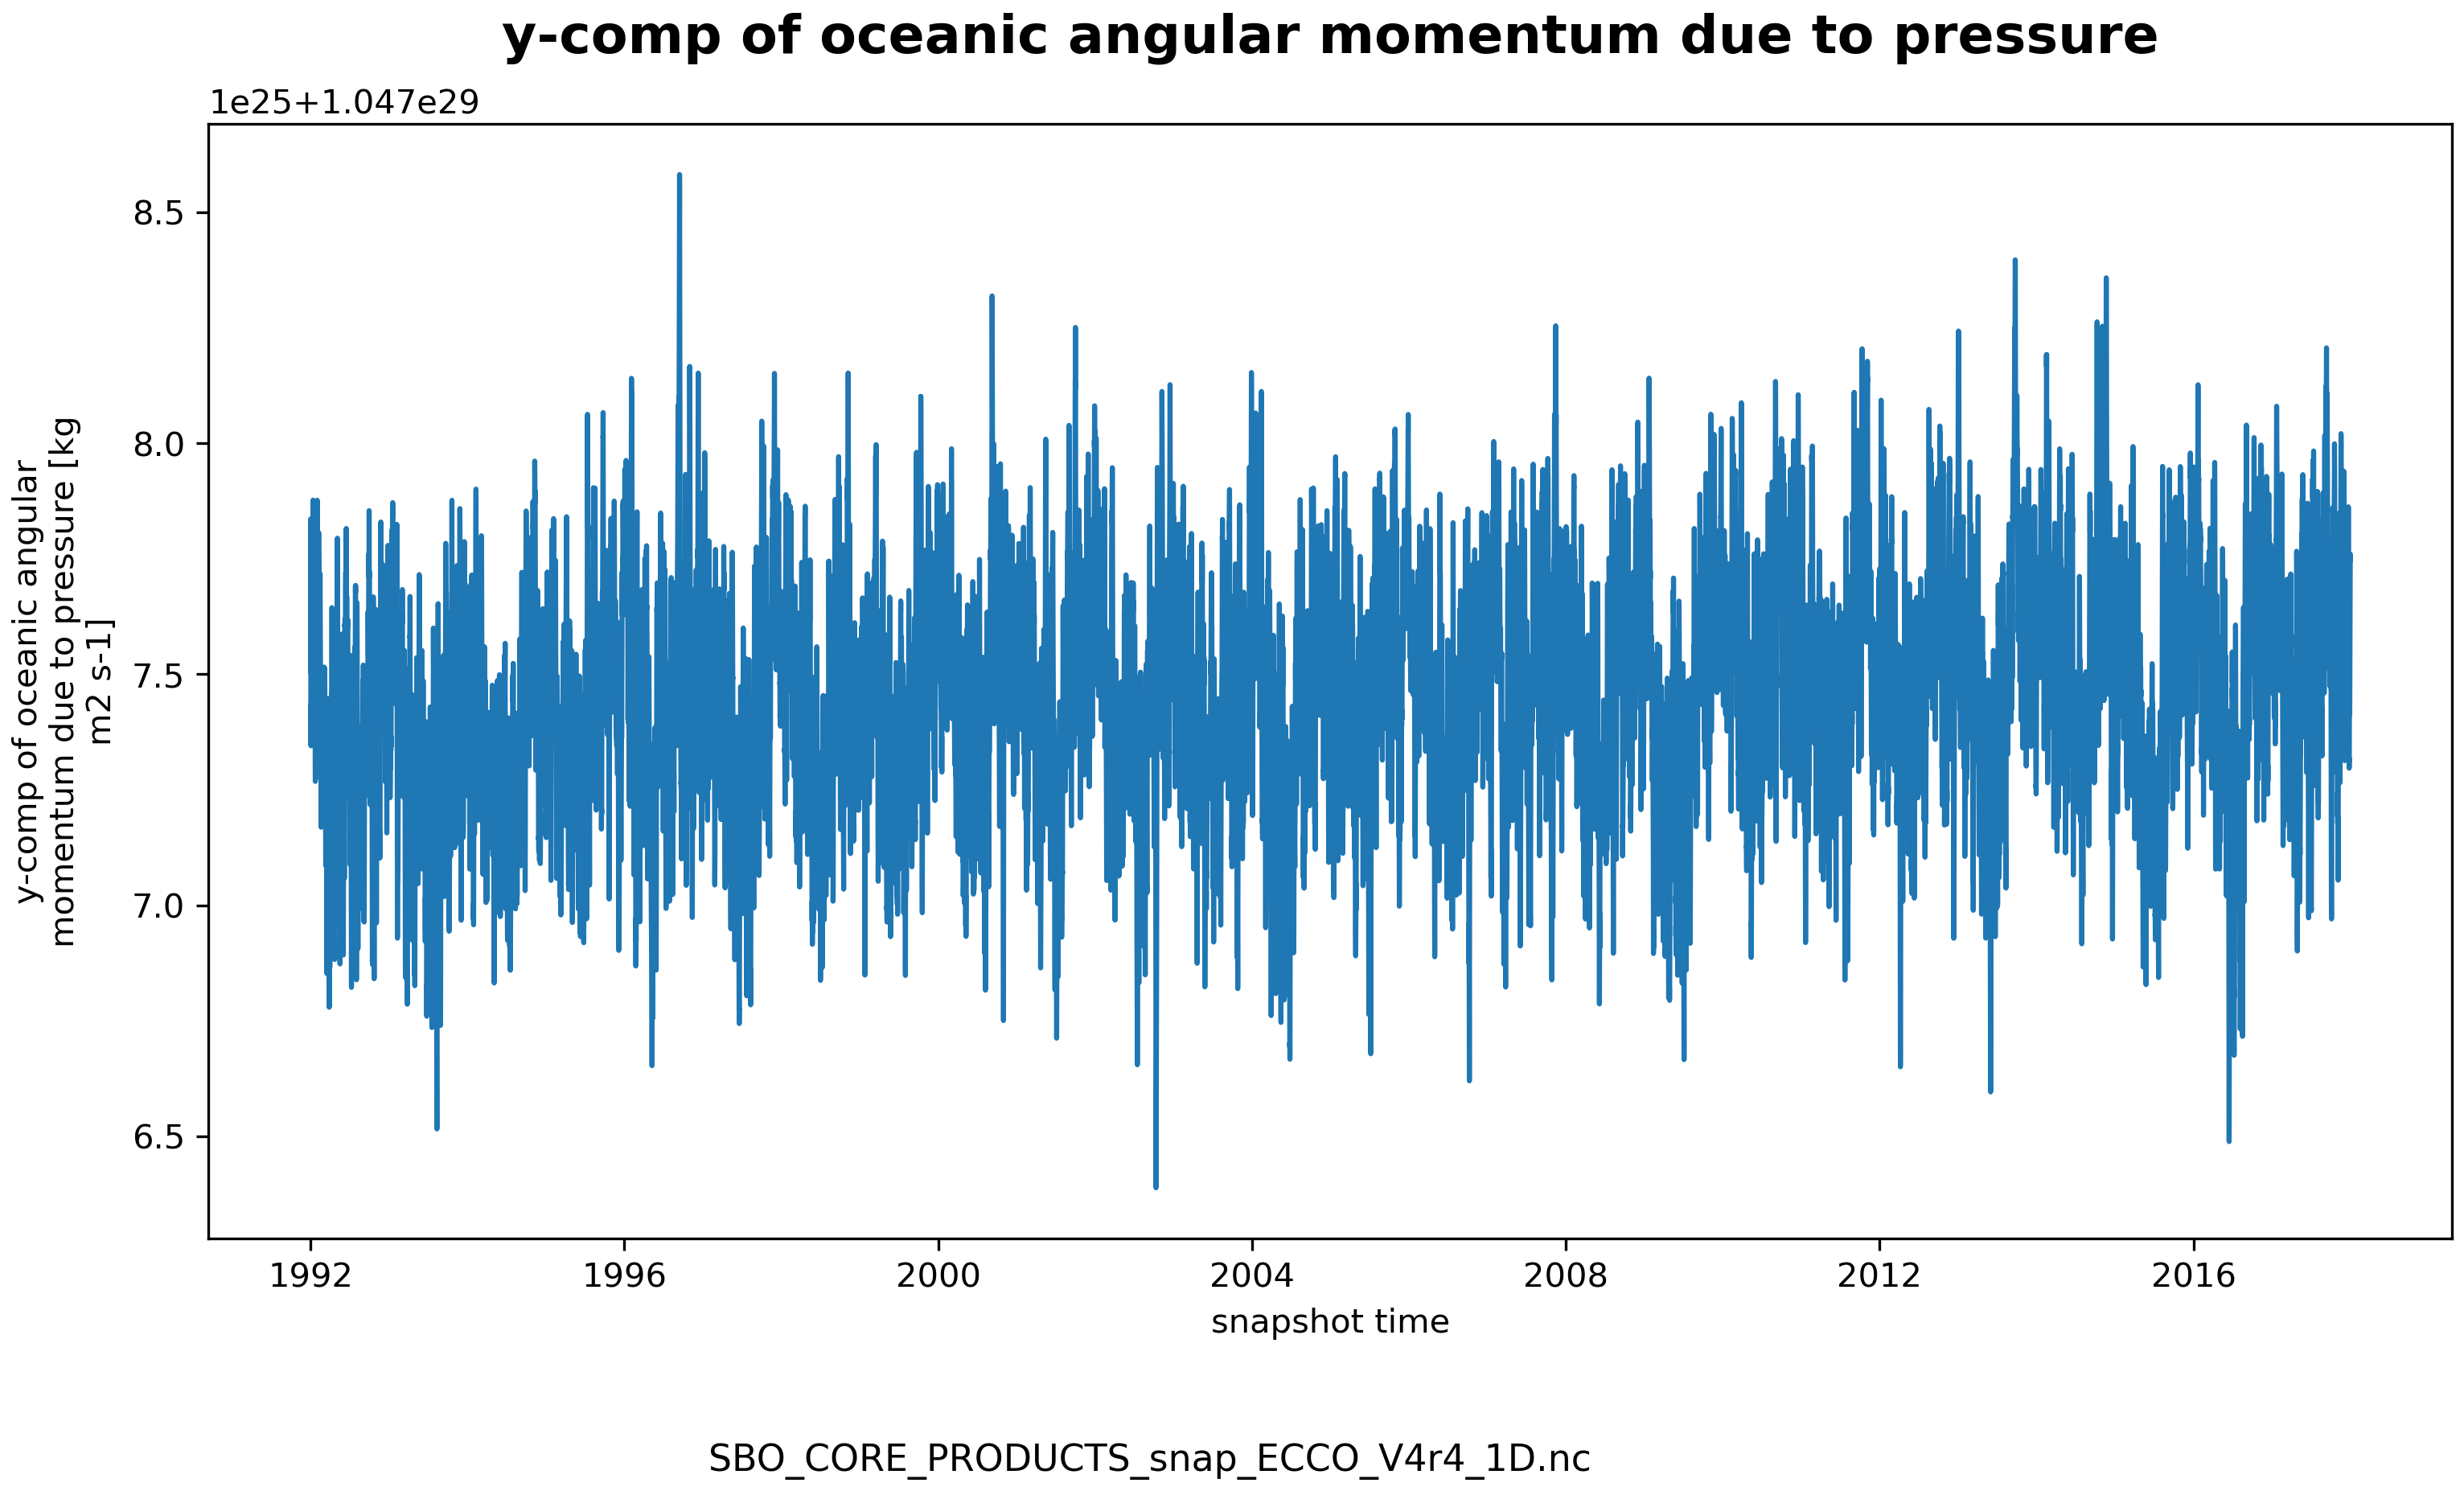
\includegraphics[scale=0.55]{../images/plots/v4r4/oneD_plots/SBO_Core_Products/yoamp.png}
\caption{Dataset: SBO\_CORE\_PRODUCTS, Variable: yoamp}
\label{tab:table-SBO_CORE_PRODUCTS_yoamp-Plot}
\end{figure}
\newpage
\pagebreak
\subsubsection{1D Variable: yoamp\_dsl}
\begin{longtable}{|m{0.06\textwidth}|m{0.3\textwidth}|m{0.45\textwidth}|m{0.12\textwidth}|}
\caption{Attributes description of the variable 'yoamp\_dsl' from SBO\_CORE\_PRODUCTS's  dataset.}
\label{tab:table-SBO_CORE_PRODUCTS_yoamp_dsl} \\ 
\hline \endhead \hline \endfoot
\rowcolor{lightgray} \textbf{Storage Type} & \textbf{Variable Name} & \textbf{Description} & \textbf{Unit} \\ \hline
float64 & yoamp\_dsl & Y-comp of oceanic angular momentum due to pressure based on dynamic (ib-corrected) sea level & kg m2 s-1 \\ \hline
\multicolumn{4}{|c|}{\cellcolor{lightgray}{\textbf{Description of the variable in Common Data language (CDL)}}} \\ \hline
\multicolumn{4}{|c|}{\fontfamily{lmtt}\selectfont{\makecell{\parbox{.95\textwidth}{\vspace*{0.25cm} \footnotesize{float64 yoamp\_dsl(time)\\
\hspace*{0.5cm}yoamp\_dsl: \_FillValue = 9.969209968386869e+36\\
\hspace*{0.5cm}yoamp\_dsl: coordinates = time\\
\hspace*{0.5cm}yoamp\_dsl: coverage\_content\_type = modelResult\\
\hspace*{0.5cm}yoamp\_dsl: long\_name = y-comp of oceanic angular momentum due to pressure based on dynamic (IB-corrected) sea level\\
\hspace*{0.5cm}yoamp\_dsl: units = kg m2 s-1\\
\hspace*{0.5cm}yoamp\_dsl: valid\_max = 1.0478187262074598e+29\\
\hspace*{0.5cm}yoamp\_dsl: valid\_min = 1.0476994334049981e+29\\
}}}}} \\ \hline
\rowcolor{lightgray} \multicolumn{4}{|c|}{\textbf{Comments}} \\ \hline
\multicolumn{4}{|p{1\textwidth}|}{\footnotesize{{N/a}}} \\ \hline
\end{longtable}

\begin{figure}[H]
\centering
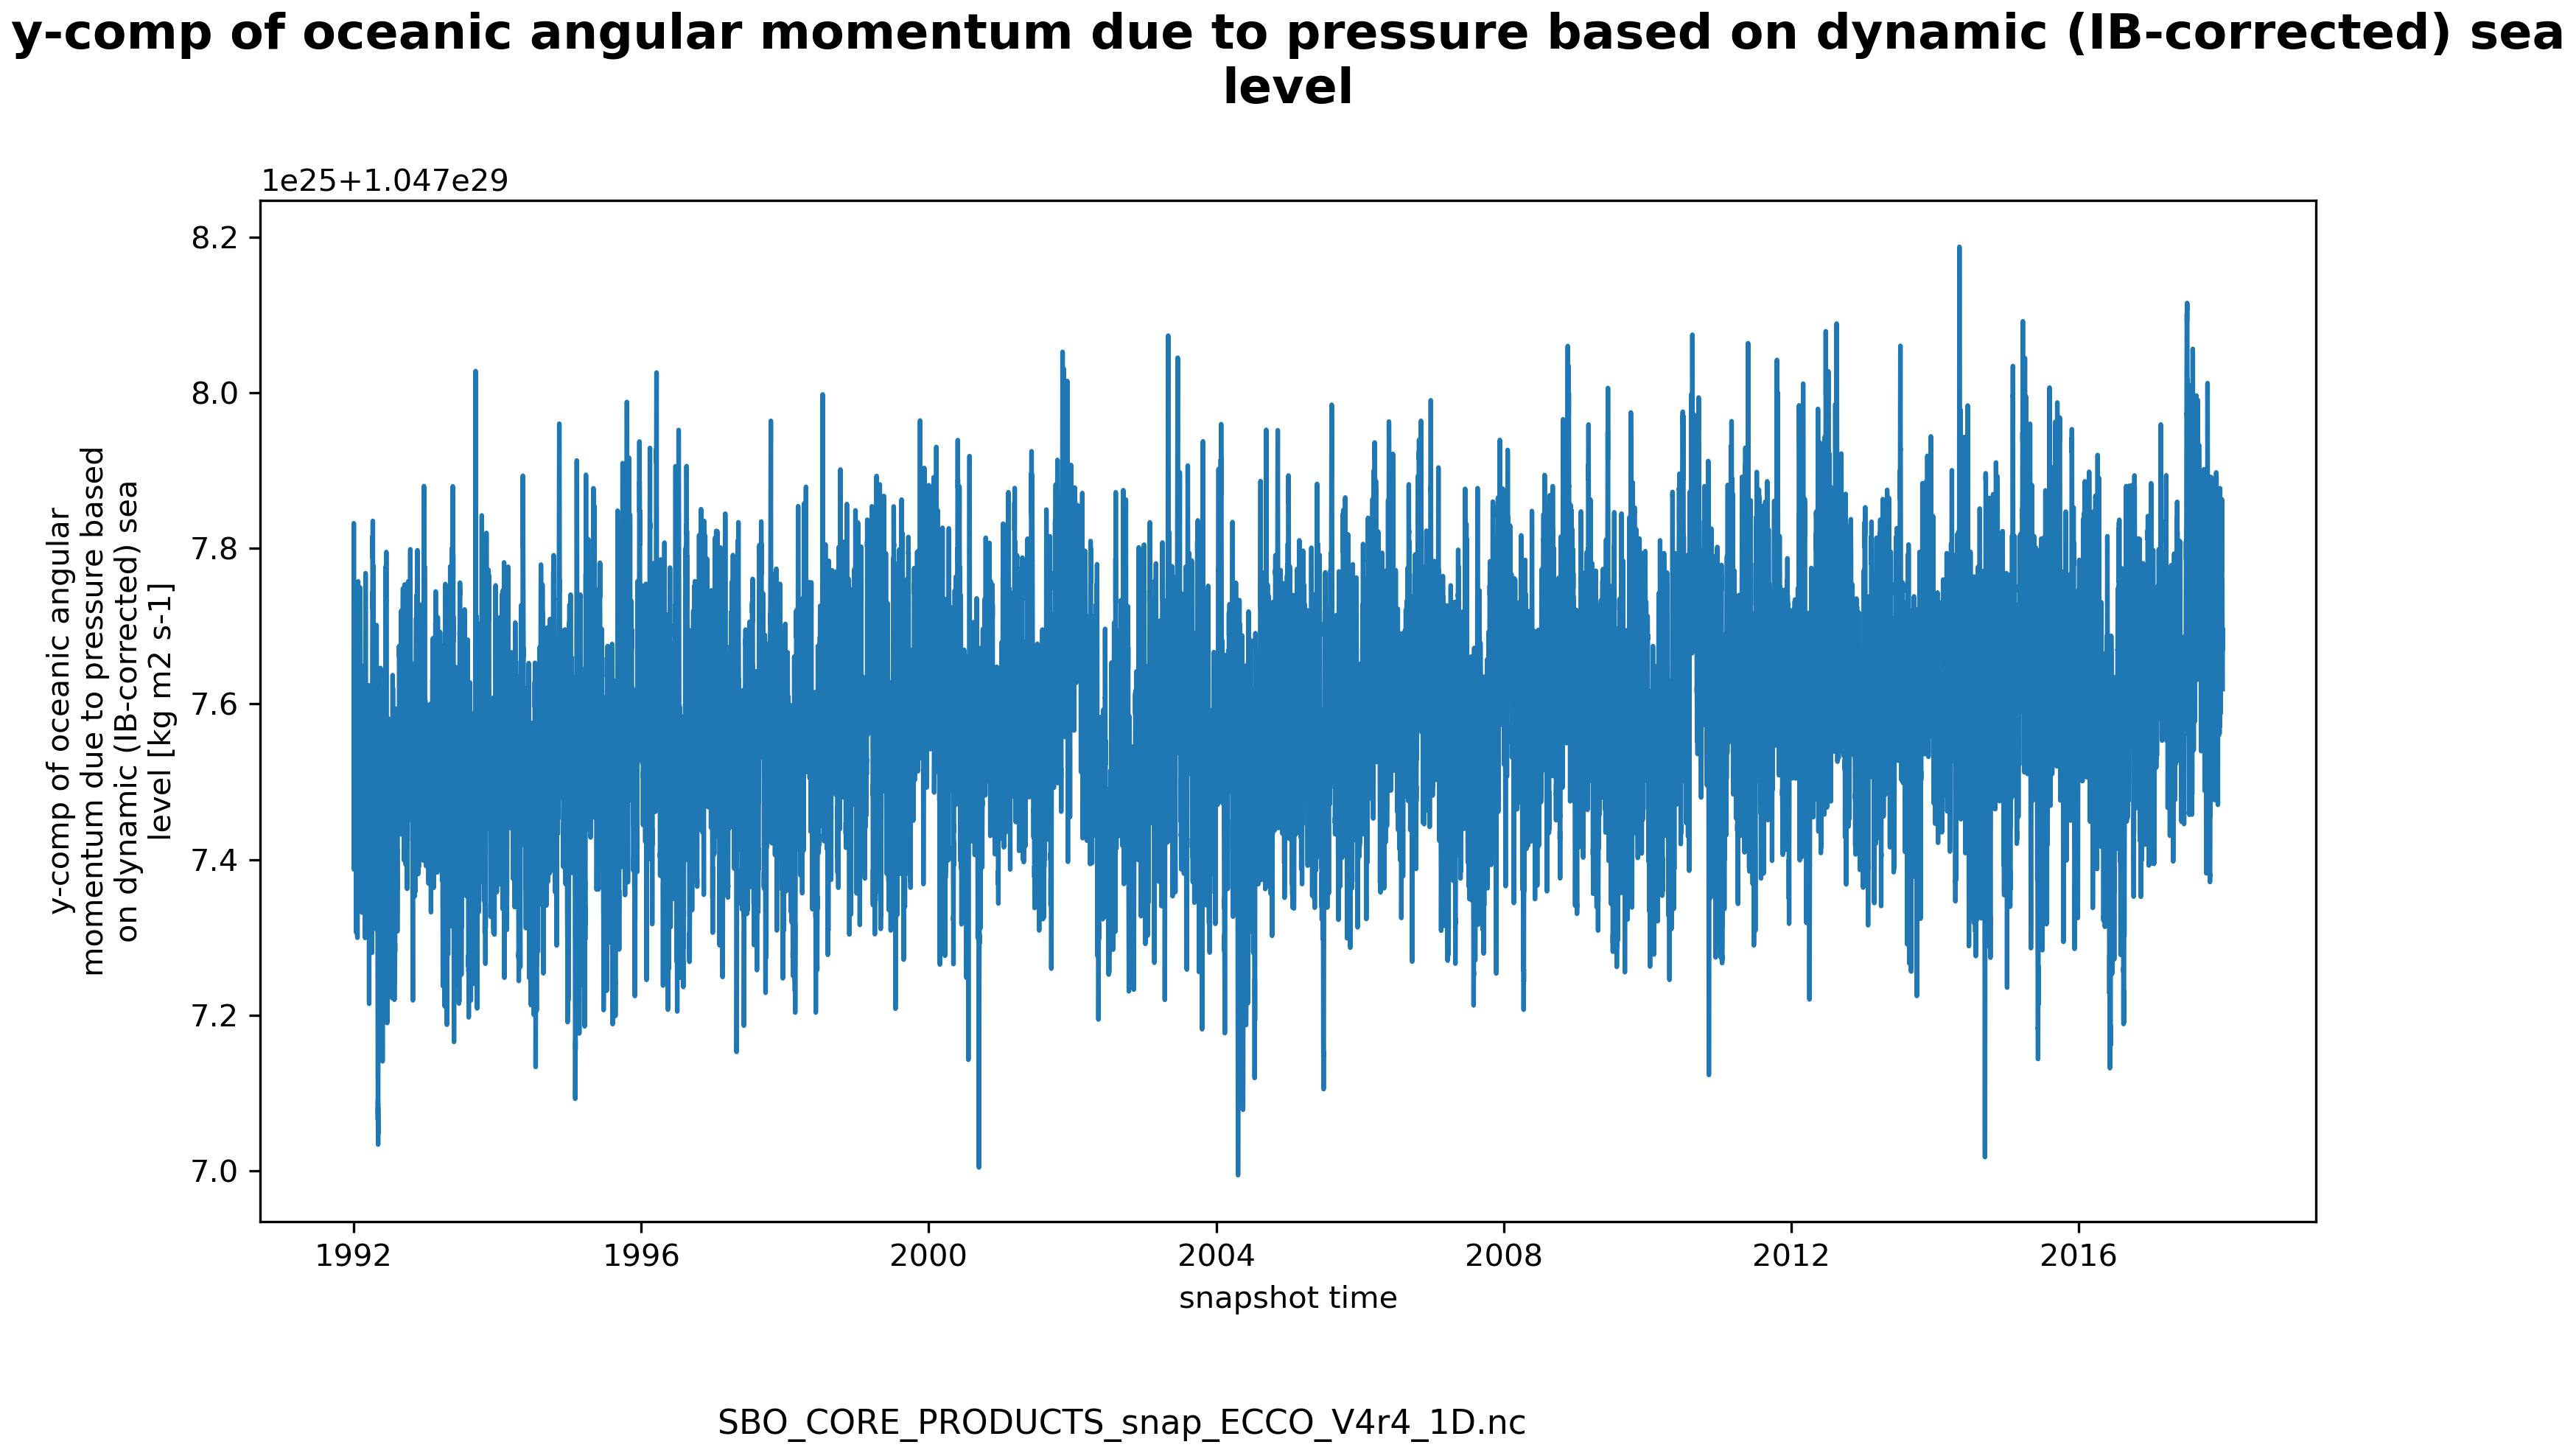
\includegraphics[scale=0.55]{../images/plots/v4r4/oneD_plots/SBO_Core_Products/yoamp_dsl.png}
\caption{Dataset: SBO\_CORE\_PRODUCTS, Variable: yoamp\_dsl}
\label{tab:table-SBO_CORE_PRODUCTS_yoamp_dsl-Plot}
\end{figure}
\newpage
\pagebreak
\subsubsection{1D Variable: yoamp\_fw}
\begin{longtable}{|m{0.06\textwidth}|m{0.3\textwidth}|m{0.45\textwidth}|m{0.12\textwidth}|}
\caption{Attributes description of the variable 'yoamp\_fw' from SBO\_CORE\_PRODUCTS's  dataset.}
\label{tab:table-SBO_CORE_PRODUCTS_yoamp_fw} \\ 
\hline \endhead \hline \endfoot
\rowcolor{lightgray} \textbf{Storage Type} & \textbf{Variable Name} & \textbf{Description} & \textbf{Unit} \\ \hline
float64 & yoamp\_fw & Y-comp of oceanic angular momentum due to freshwater flux & kg m2 s-1 \\ \hline
\multicolumn{4}{|c|}{\cellcolor{lightgray}{\textbf{Description of the variable in Common Data language (CDL)}}} \\ \hline
\multicolumn{4}{|c|}{\fontfamily{lmtt}\selectfont{\makecell{\parbox{.95\textwidth}{\vspace*{0.25cm} \footnotesize{float64 yoamp\_fw(time)\\
\hspace*{0.5cm}yoamp\_fw: \_FillValue = 9.969209968386869e+36\\
\hspace*{0.5cm}yoamp\_fw: coordinates = time\\
\hspace*{0.5cm}yoamp\_fw: coverage\_content\_type = modelResult\\
\hspace*{0.5cm}yoamp\_fw: long\_name = y-comp of oceanic angular momentum due to freshwater flux\\
\hspace*{0.5cm}yoamp\_fw: units = kg m2 s-1\\
\hspace*{0.5cm}yoamp\_fw: valid\_max = 4.872705717529432e+24\\
\hspace*{0.5cm}yoamp\_fw: valid\_min = 2.6255410225894626e+24\\
}}}}} \\ \hline
\rowcolor{lightgray} \multicolumn{4}{|c|}{\textbf{Comments}} \\ \hline
\multicolumn{4}{|p{1\textwidth}|}{\footnotesize{{N/a}}} \\ \hline
\end{longtable}

\begin{figure}[H]
\centering
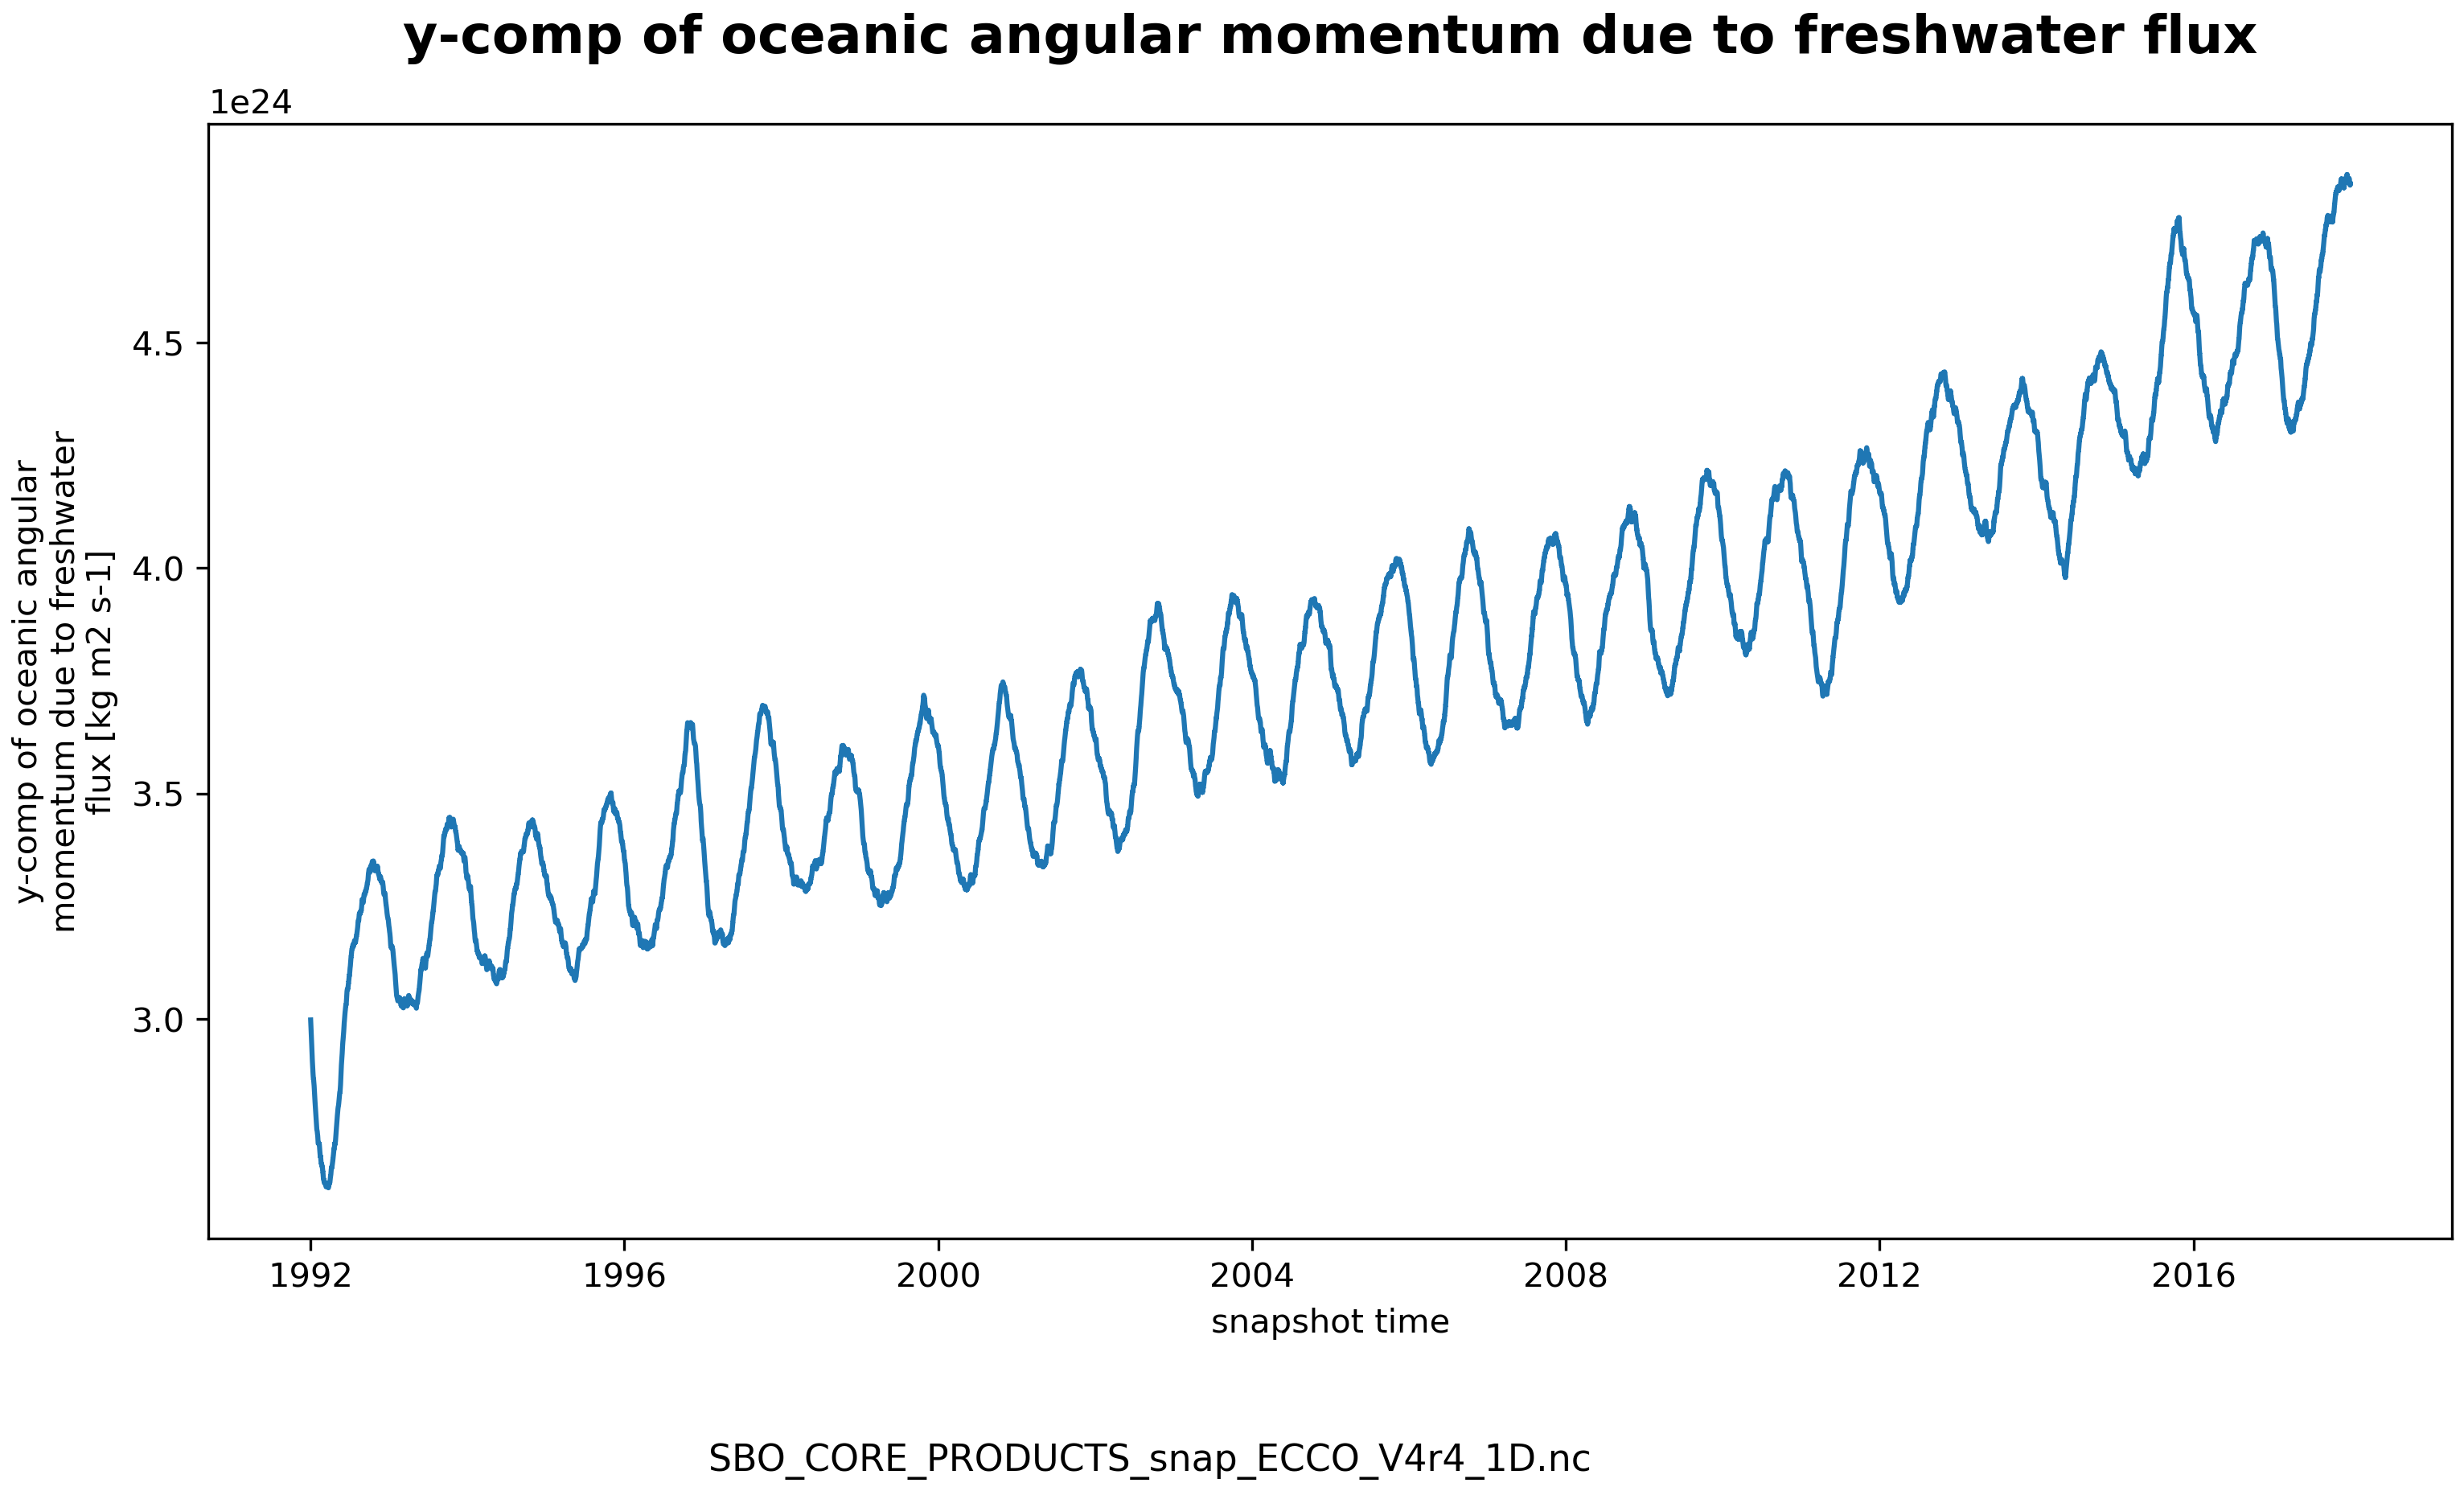
\includegraphics[scale=0.55]{../images/plots/v4r4/oneD_plots/SBO_Core_Products/yoamp_fw.png}
\caption{Dataset: SBO\_CORE\_PRODUCTS, Variable: yoamp\_fw}
\label{tab:table-SBO_CORE_PRODUCTS_yoamp_fw-Plot}
\end{figure}
\newpage
\pagebreak
\subsubsection{1D Variable: zcom}
\begin{longtable}{|m{0.06\textwidth}|m{0.3\textwidth}|m{0.45\textwidth}|m{0.12\textwidth}|}
\caption{Attributes description of the variable 'zcom' from SBO\_CORE\_PRODUCTS's  dataset.}
\label{tab:table-SBO_CORE_PRODUCTS_zcom} \\ 
\hline \endhead \hline \endfoot
\rowcolor{lightgray} \textbf{Storage Type} & \textbf{Variable Name} & \textbf{Description} & \textbf{Unit} \\ \hline
float64 & zcom & Z-comp of center-of-mass of ocean & m \\ \hline
\multicolumn{4}{|c|}{\cellcolor{lightgray}{\textbf{Description of the variable in Common Data language (CDL)}}} \\ \hline
\multicolumn{4}{|c|}{\fontfamily{lmtt}\selectfont{\makecell{\parbox{.95\textwidth}{\vspace*{0.25cm} \footnotesize{float64 zcom(time)\\
\hspace*{0.5cm}zcom: \_FillValue = 9.969209968386869e+36\\
\hspace*{0.5cm}zcom: coordinates = time\\
\hspace*{0.5cm}zcom: coverage\_content\_type = modelResult\\
\hspace*{0.5cm}zcom: long\_name = z-comp of center-of-mass of ocean\\
\hspace*{0.5cm}zcom: units = m\\
\hspace*{0.5cm}zcom: valid\_max = -875350.3238026679\\
\hspace*{0.5cm}zcom: valid\_min = -875420.3898804963\\
}}}}} \\ \hline
\rowcolor{lightgray} \multicolumn{4}{|c|}{\textbf{Comments}} \\ \hline
\multicolumn{4}{|p{1\textwidth}|}{\footnotesize{{N/a}}} \\ \hline
\end{longtable}

\begin{figure}[H]
\centering
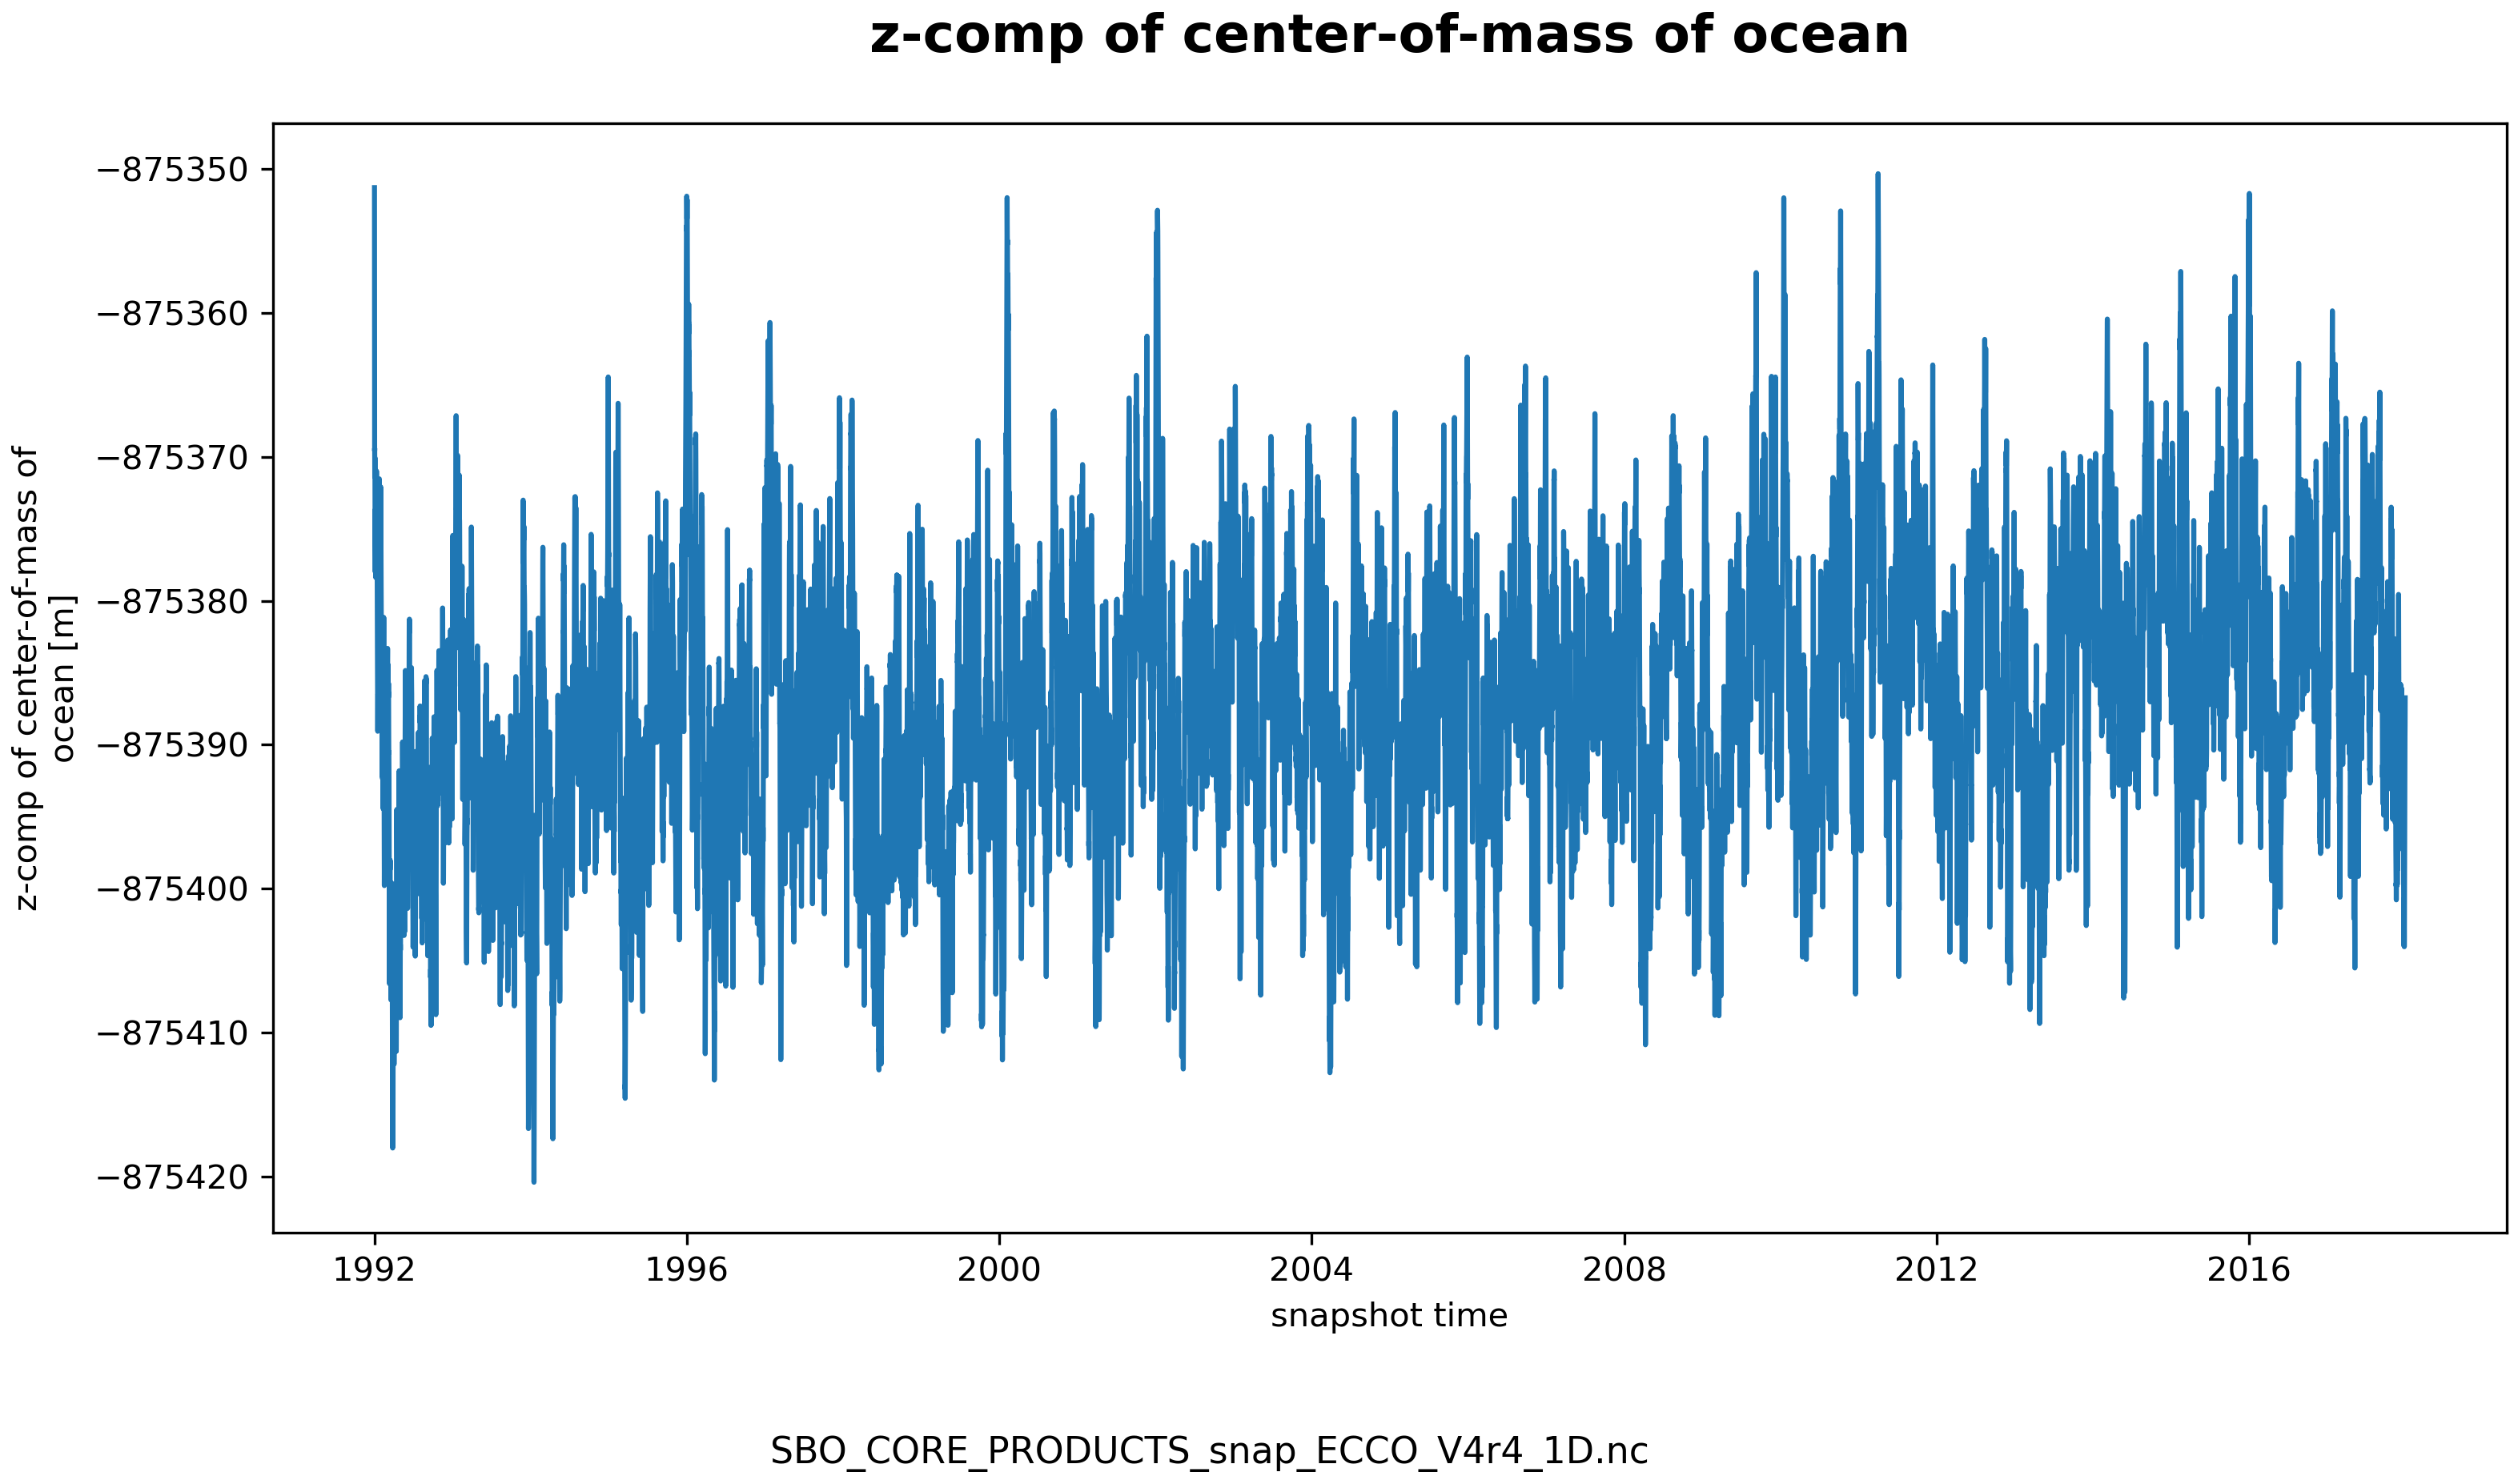
\includegraphics[scale=0.55]{../images/plots/v4r4/oneD_plots/SBO_Core_Products/zcom.png}
\caption{Dataset: SBO\_CORE\_PRODUCTS, Variable: zcom}
\label{tab:table-SBO_CORE_PRODUCTS_zcom-Plot}
\end{figure}
\newpage
\pagebreak
\subsubsection{1D Variable: zcom\_fw}
\begin{longtable}{|m{0.06\textwidth}|m{0.3\textwidth}|m{0.45\textwidth}|m{0.12\textwidth}|}
\caption{Attributes description of the variable 'zcom\_fw' from SBO\_CORE\_PRODUCTS's  dataset.}
\label{tab:table-SBO_CORE_PRODUCTS_zcom_fw} \\ 
\hline \endhead \hline \endfoot
\rowcolor{lightgray} \textbf{Storage Type} & \textbf{Variable Name} & \textbf{Description} & \textbf{Unit} \\ \hline
float64 & zcom\_fw & Z-comp of center-of-mass of freshater flux & m \\ \hline
\multicolumn{4}{|c|}{\cellcolor{lightgray}{\textbf{Description of the variable in Common Data language (CDL)}}} \\ \hline
\multicolumn{4}{|c|}{\fontfamily{lmtt}\selectfont{\makecell{\parbox{.95\textwidth}{\vspace*{0.25cm} \footnotesize{float64 zcom\_fw(time)\\
\hspace*{0.5cm}zcom\_fw: \_FillValue = 9.969209968386869e+36\\
\hspace*{0.5cm}zcom\_fw: coordinates = time\\
\hspace*{0.5cm}zcom\_fw: coverage\_content\_type = modelResult\\
\hspace*{0.5cm}zcom\_fw: long\_name = z-comp of center-of-mass of freshater flux\\
\hspace*{0.5cm}zcom\_fw: units = m\\
\hspace*{0.5cm}zcom\_fw: valid\_max = -648386.5781734567\\
\hspace*{0.5cm}zcom\_fw: valid\_min = -648386.5781734617\\
}}}}} \\ \hline
\rowcolor{lightgray} \multicolumn{4}{|c|}{\textbf{Comments}} \\ \hline
\multicolumn{4}{|p{1\textwidth}|}{\footnotesize{{N/a}}} \\ \hline
\end{longtable}

\begin{figure}[H]
\centering
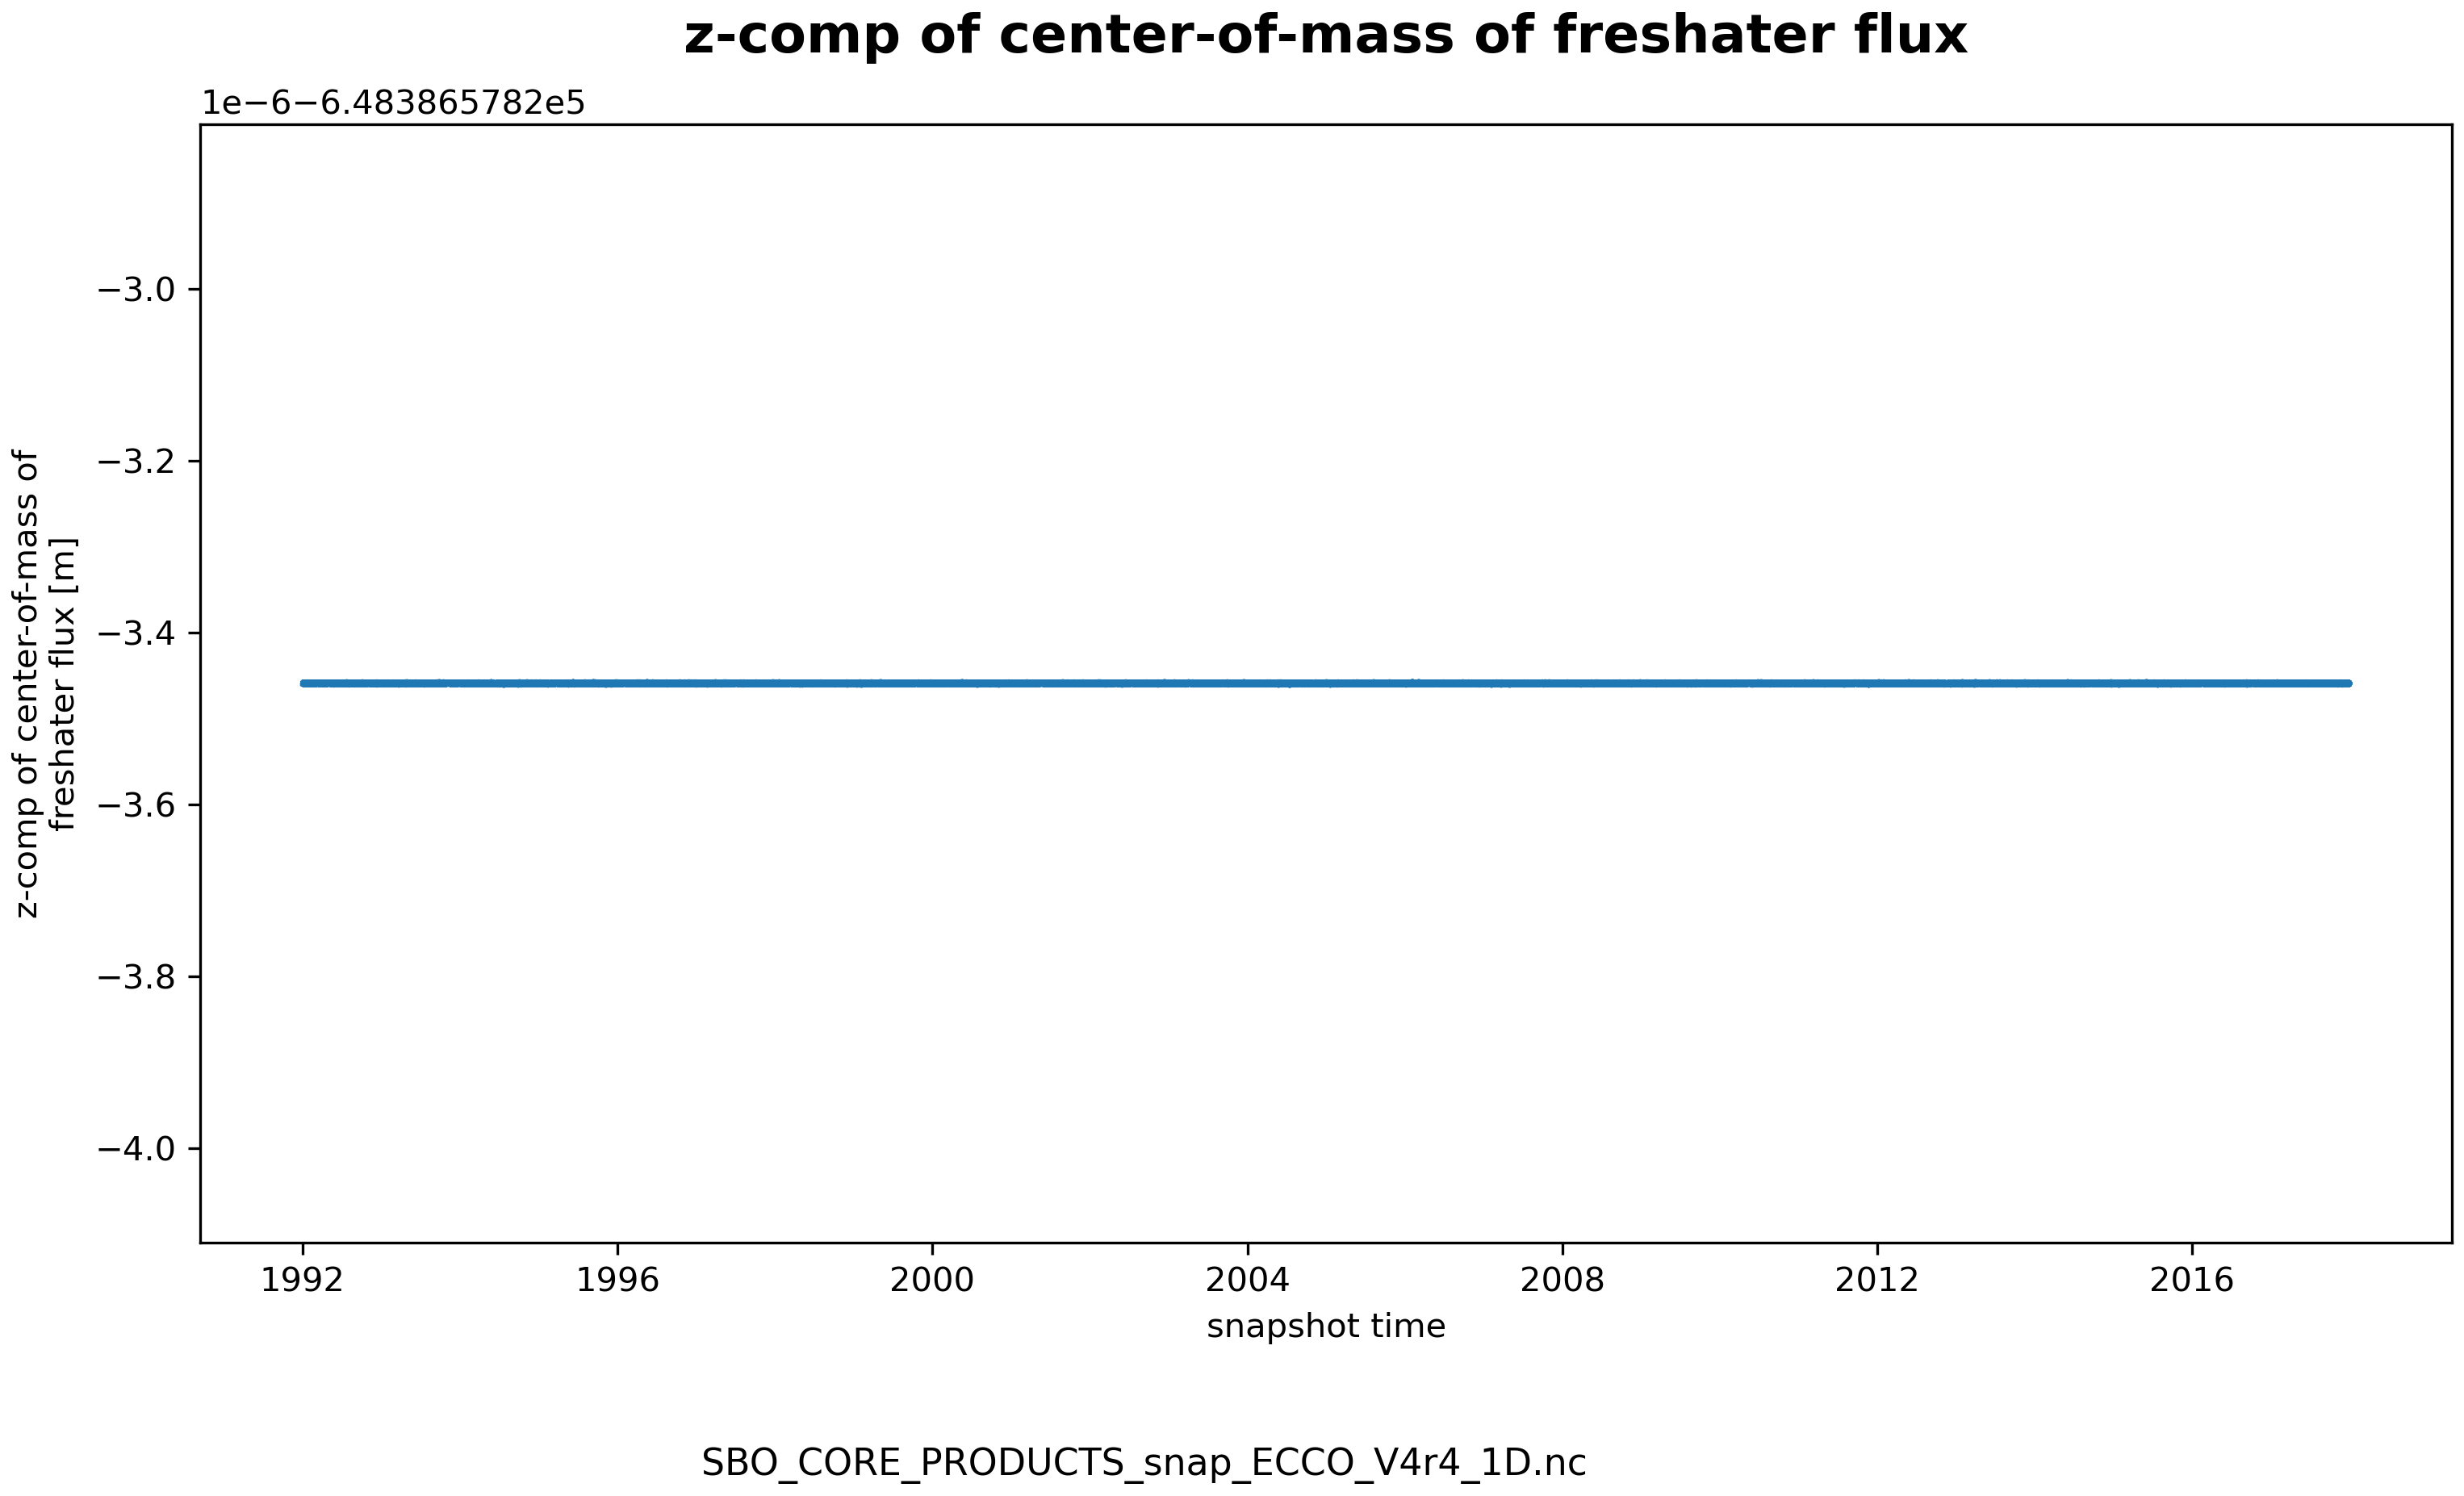
\includegraphics[scale=0.55]{../images/plots/v4r4/oneD_plots/SBO_Core_Products/zcom_fw.png}
\caption{Dataset: SBO\_CORE\_PRODUCTS, Variable: zcom\_fw}
\label{tab:table-SBO_CORE_PRODUCTS_zcom_fw-Plot}
\end{figure}
\newpage
\pagebreak
\subsubsection{1D Variable: zoamc}
\begin{longtable}{|m{0.06\textwidth}|m{0.3\textwidth}|m{0.45\textwidth}|m{0.12\textwidth}|}
\caption{Attributes description of the variable 'zoamc' from SBO\_CORE\_PRODUCTS's  dataset.}
\label{tab:table-SBO_CORE_PRODUCTS_zoamc} \\ 
\hline \endhead \hline \endfoot
\rowcolor{lightgray} \textbf{Storage Type} & \textbf{Variable Name} & \textbf{Description} & \textbf{Unit} \\ \hline
float64 & zoamc & Z-comp of oceanic angular momentum due to currents & kg m2 s-1 \\ \hline
\multicolumn{4}{|c|}{\cellcolor{lightgray}{\textbf{Description of the variable in Common Data language (CDL)}}} \\ \hline
\multicolumn{4}{|c|}{\fontfamily{lmtt}\selectfont{\makecell{\parbox{.95\textwidth}{\vspace*{0.25cm} \footnotesize{float64 zoamc(time)\\
\hspace*{0.5cm}zoamc: \_FillValue = 9.969209968386869e+36\\
\hspace*{0.5cm}zoamc: coordinates = time\\
\hspace*{0.5cm}zoamc: coverage\_content\_type = modelResult\\
\hspace*{0.5cm}zoamc: long\_name = z-comp of oceanic angular momentum due to currents\\
\hspace*{0.5cm}zoamc: units = kg m2 s-1\\
\hspace*{0.5cm}zoamc: valid\_max = 2.207264300276968e+25\\
\hspace*{0.5cm}zoamc: valid\_min = 7.331764457927521e+24\\
}}}}} \\ \hline
\rowcolor{lightgray} \multicolumn{4}{|c|}{\textbf{Comments}} \\ \hline
\multicolumn{4}{|p{1\textwidth}|}{\footnotesize{{N/a}}} \\ \hline
\end{longtable}

\begin{figure}[H]
\centering
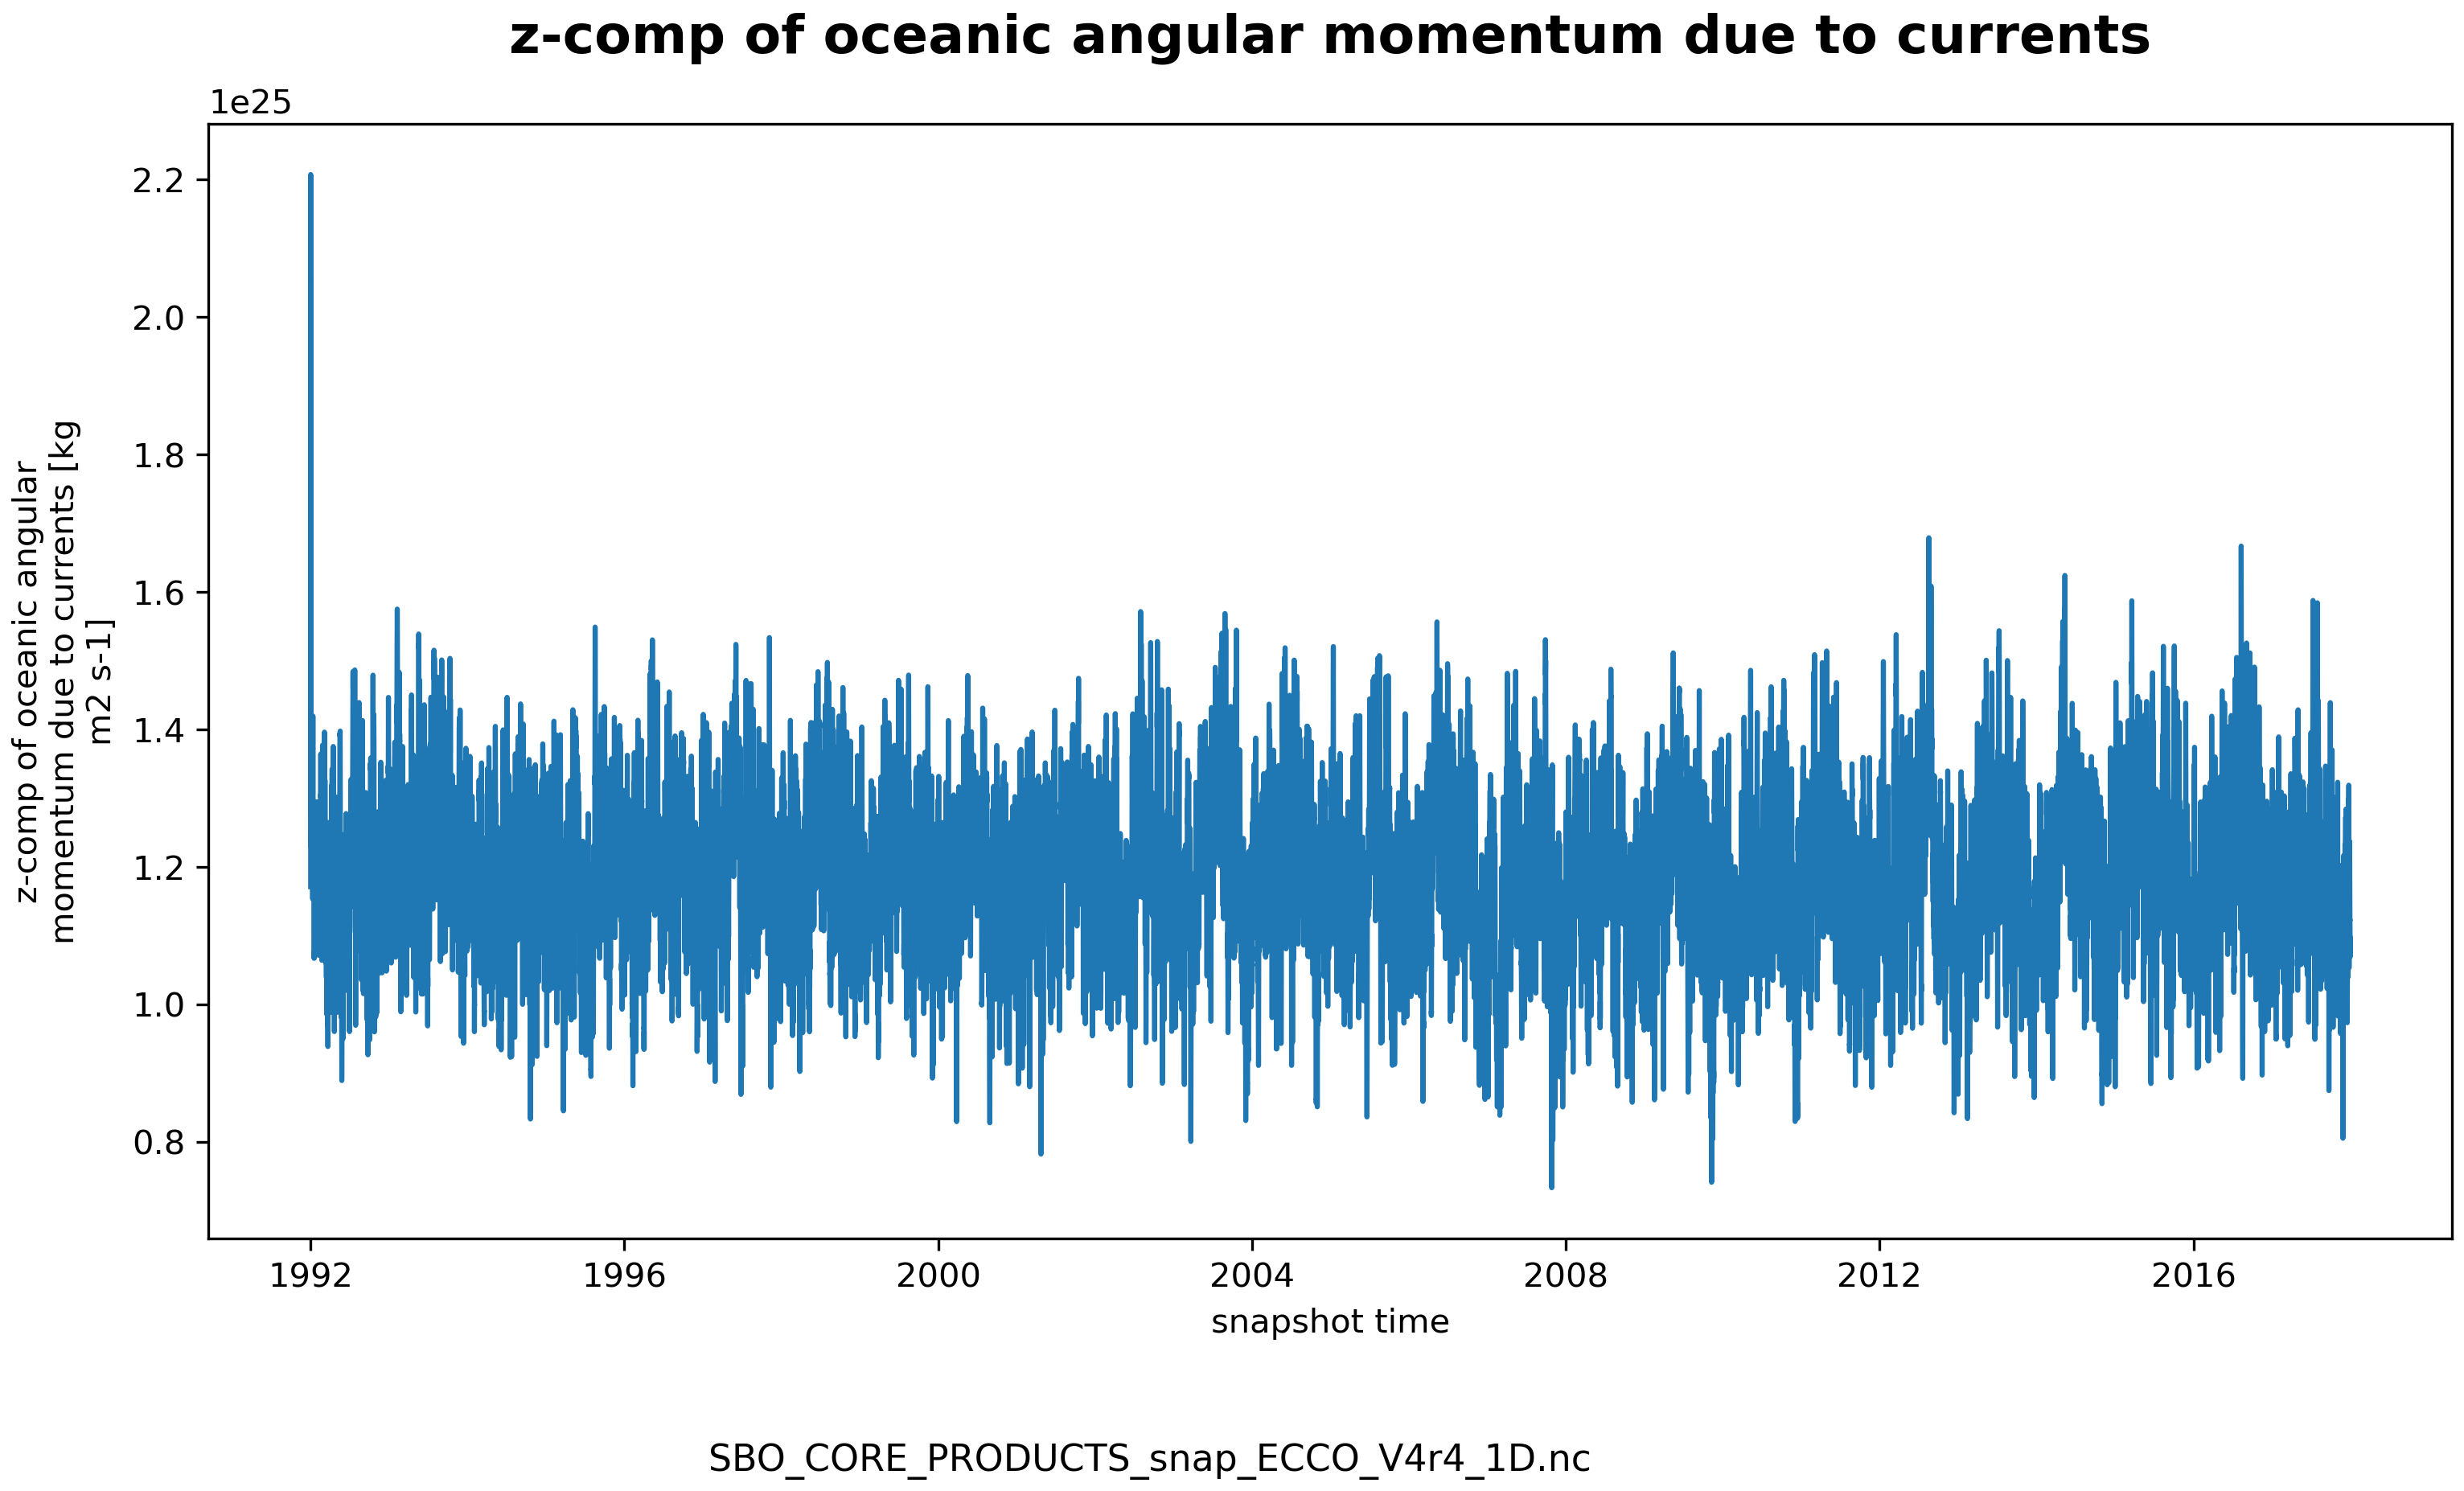
\includegraphics[scale=0.55]{../images/plots/v4r4/oneD_plots/SBO_Core_Products/zoamc.png}
\caption{Dataset: SBO\_CORE\_PRODUCTS, Variable: zoamc}
\label{tab:table-SBO_CORE_PRODUCTS_zoamc-Plot}
\end{figure}
\newpage
\pagebreak
\subsubsection{1D Variable: zoamc\_si}
\begin{longtable}{|m{0.06\textwidth}|m{0.3\textwidth}|m{0.45\textwidth}|m{0.12\textwidth}|}
\caption{Attributes description of the variable 'zoamc\_si' from SBO\_CORE\_PRODUCTS's  dataset.}
\label{tab:table-SBO_CORE_PRODUCTS_zoamc_si} \\ 
\hline \endhead \hline \endfoot
\rowcolor{lightgray} \textbf{Storage Type} & \textbf{Variable Name} & \textbf{Description} & \textbf{Unit} \\ \hline
float64 & zoamc\_si & Z-comp of oceanic angular momentum due to sea-ice motion & kg m2 s-1 \\ \hline
\multicolumn{4}{|c|}{\cellcolor{lightgray}{\textbf{Description of the variable in Common Data language (CDL)}}} \\ \hline
\multicolumn{4}{|c|}{\fontfamily{lmtt}\selectfont{\makecell{\parbox{.95\textwidth}{\vspace*{0.25cm} \footnotesize{float64 zoamc\_si(time)\\
\hspace*{0.5cm}zoamc\_si: \_FillValue = 9.969209968386869e+36\\
\hspace*{0.5cm}zoamc\_si: coordinates = time\\
\hspace*{0.5cm}zoamc\_si: coverage\_content\_type = modelResult\\
\hspace*{0.5cm}zoamc\_si: long\_name = z-comp of oceanic angular momentum due to sea-ice motion\\
\hspace*{0.5cm}zoamc\_si: units = kg m2 s-1\\
\hspace*{0.5cm}zoamc\_si: valid\_max = 5.930388258256482e+21\\
\hspace*{0.5cm}zoamc\_si: valid\_min = -5.909426721868294e+21\\
}}}}} \\ \hline
\rowcolor{lightgray} \multicolumn{4}{|c|}{\textbf{Comments}} \\ \hline
\multicolumn{4}{|p{1\textwidth}|}{\footnotesize{{N/a}}} \\ \hline
\end{longtable}

\begin{figure}[H]
\centering
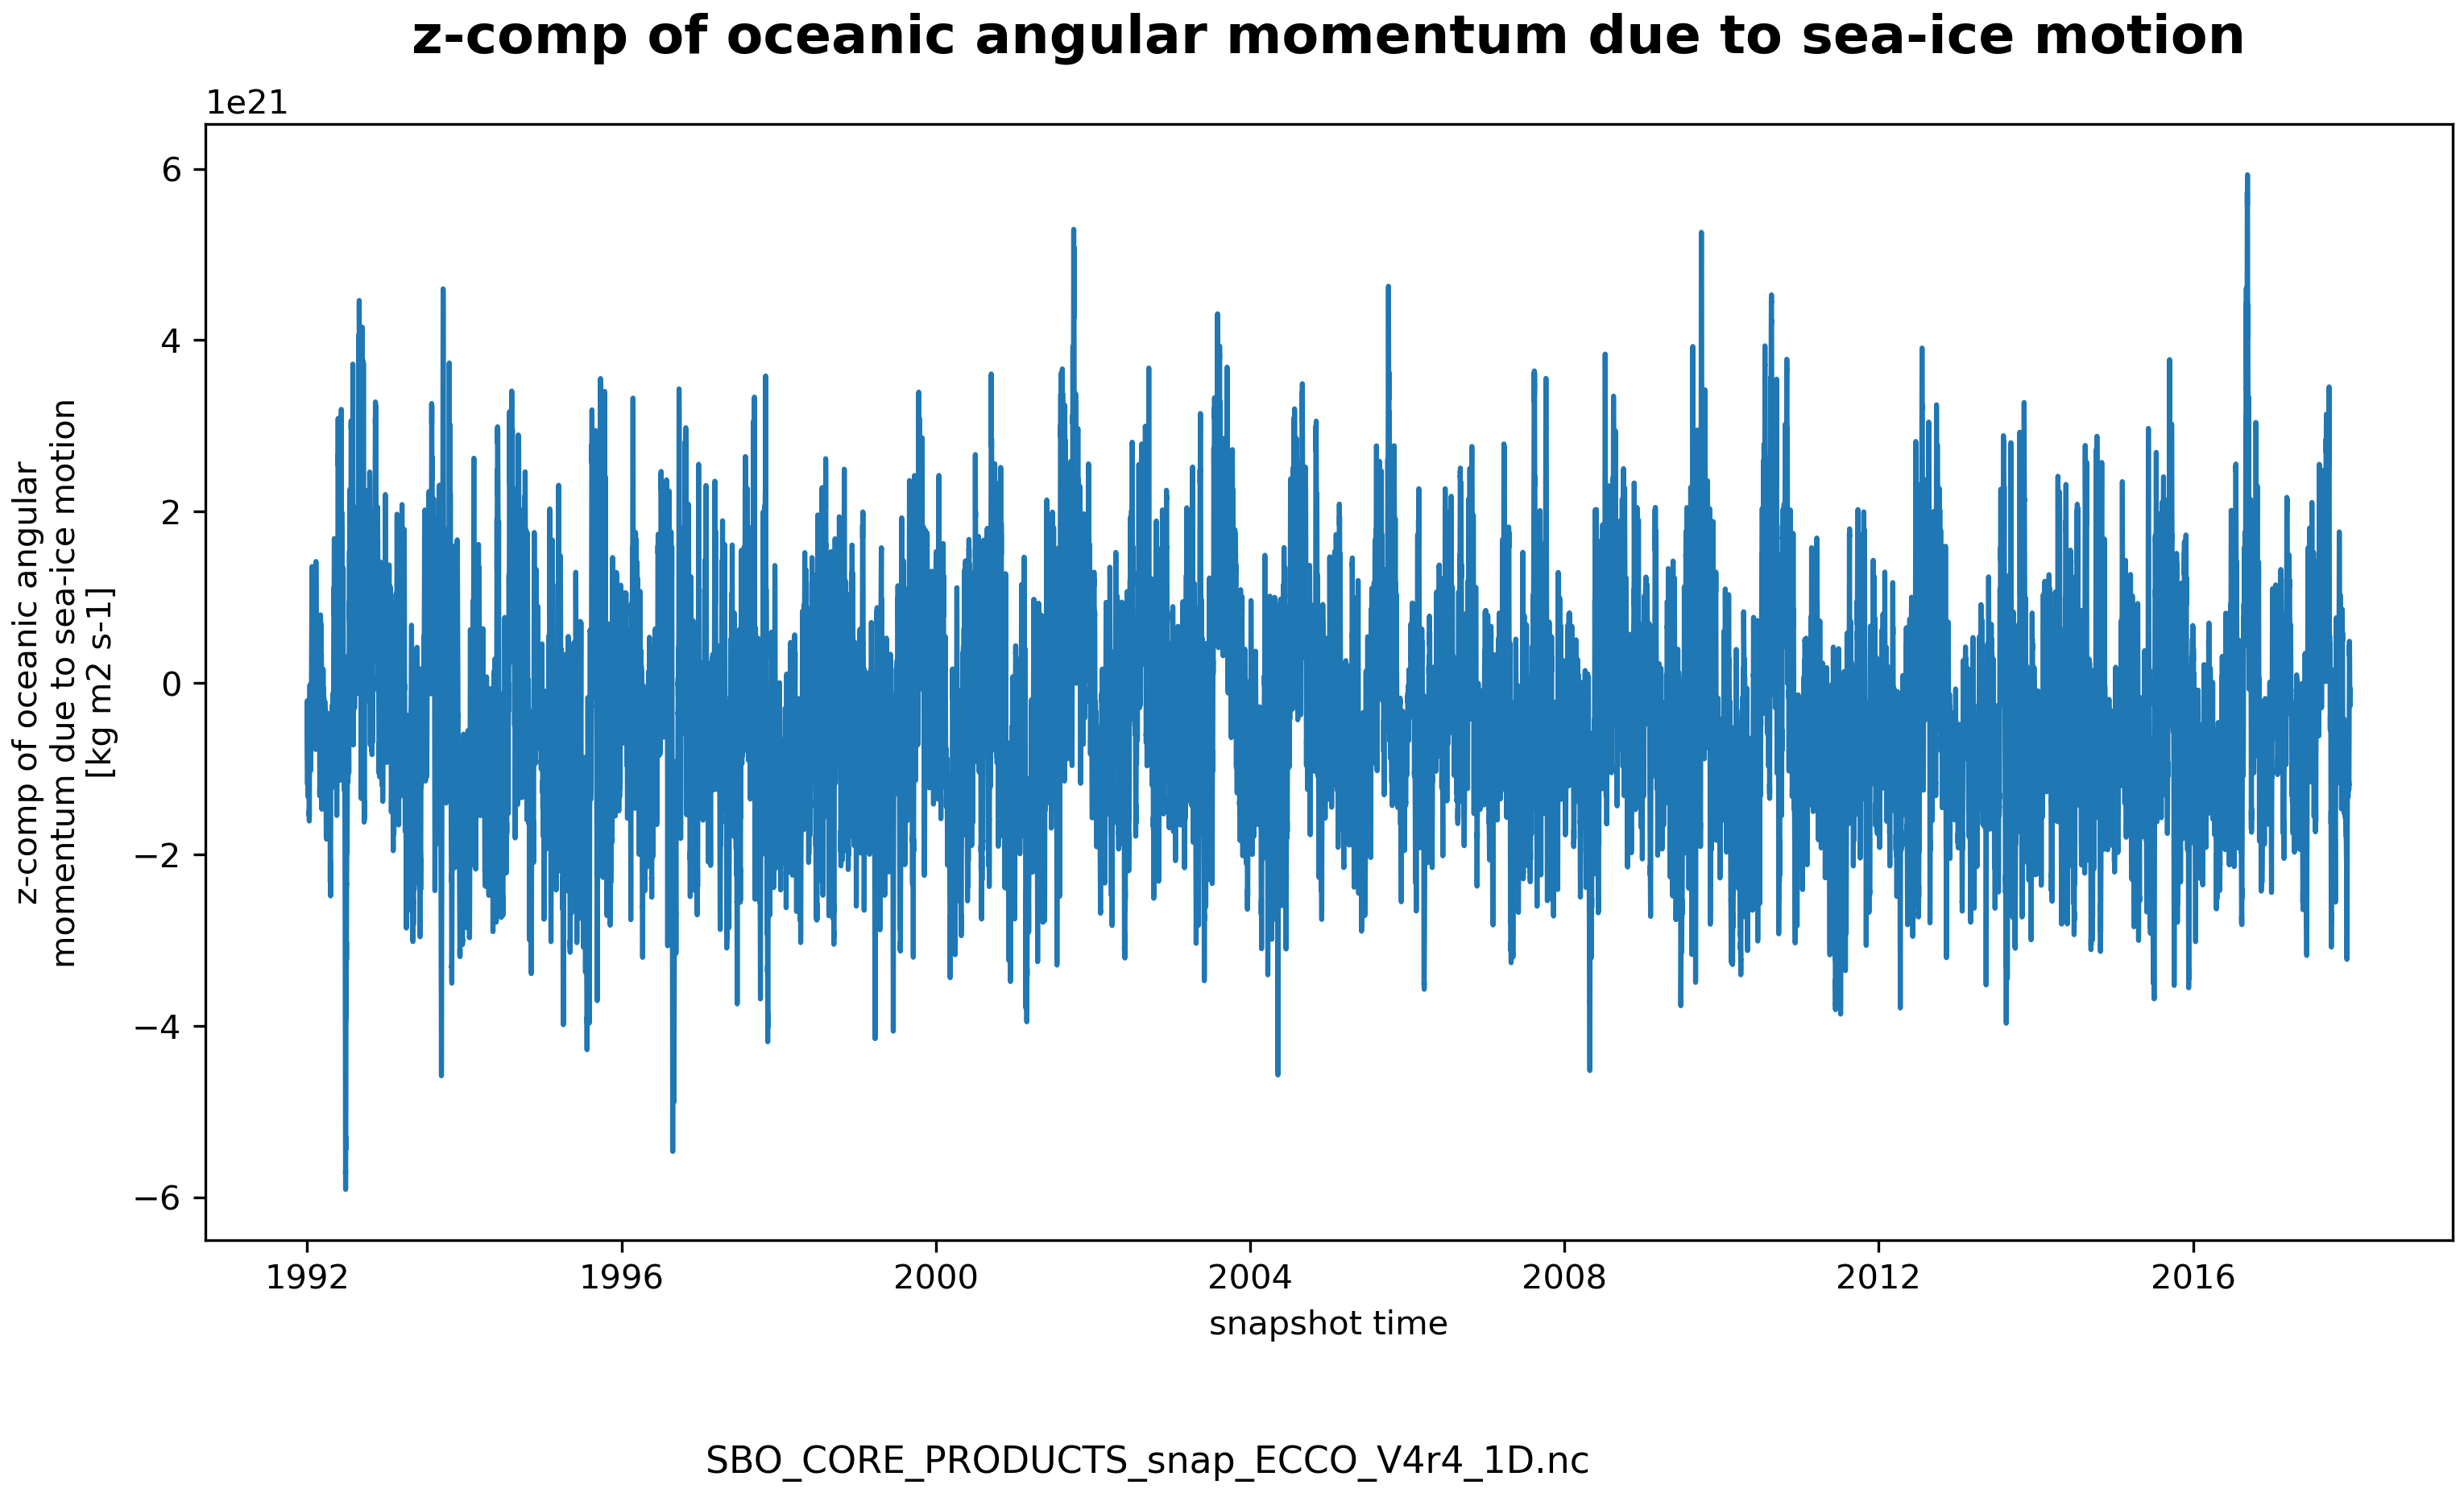
\includegraphics[scale=0.55]{../images/plots/v4r4/oneD_plots/SBO_Core_Products/zoamc_si.png}
\caption{Dataset: SBO\_CORE\_PRODUCTS, Variable: zoamc\_si}
\label{tab:table-SBO_CORE_PRODUCTS_zoamc_si-Plot}
\end{figure}
\newpage
\pagebreak
\subsubsection{1D Variable: zoamp}
\begin{longtable}{|m{0.06\textwidth}|m{0.3\textwidth}|m{0.45\textwidth}|m{0.12\textwidth}|}
\caption{Attributes description of the variable 'zoamp' from SBO\_CORE\_PRODUCTS's  dataset.}
\label{tab:table-SBO_CORE_PRODUCTS_zoamp} \\ 
\hline \endhead \hline \endfoot
\rowcolor{lightgray} \textbf{Storage Type} & \textbf{Variable Name} & \textbf{Description} & \textbf{Unit} \\ \hline
float64 & zoamp & Z-comp of oceanic angular momentum due to pressure & kg m2 s-1 \\ \hline
\multicolumn{4}{|c|}{\cellcolor{lightgray}{\textbf{Description of the variable in Common Data language (CDL)}}} \\ \hline
\multicolumn{4}{|c|}{\fontfamily{lmtt}\selectfont{\makecell{\parbox{.95\textwidth}{\vspace*{0.25cm} \footnotesize{float64 zoamp(time)\\
\hspace*{0.5cm}zoamp: \_FillValue = 9.969209968386869e+36\\
\hspace*{0.5cm}zoamp: coordinates = time\\
\hspace*{0.5cm}zoamp: coverage\_content\_type = modelResult\\
\hspace*{0.5cm}zoamp: long\_name = z-comp of oceanic angular momentum due to pressure\\
\hspace*{0.5cm}zoamp: units = kg m2 s-1\\
\hspace*{0.5cm}zoamp: valid\_max = 2.9277200254389854e+30\\
\hspace*{0.5cm}zoamp: valid\_min = 2.927645942668479e+30\\
}}}}} \\ \hline
\rowcolor{lightgray} \multicolumn{4}{|c|}{\textbf{Comments}} \\ \hline
\multicolumn{4}{|p{1\textwidth}|}{\footnotesize{{N/a}}} \\ \hline
\end{longtable}

\begin{figure}[H]
\centering
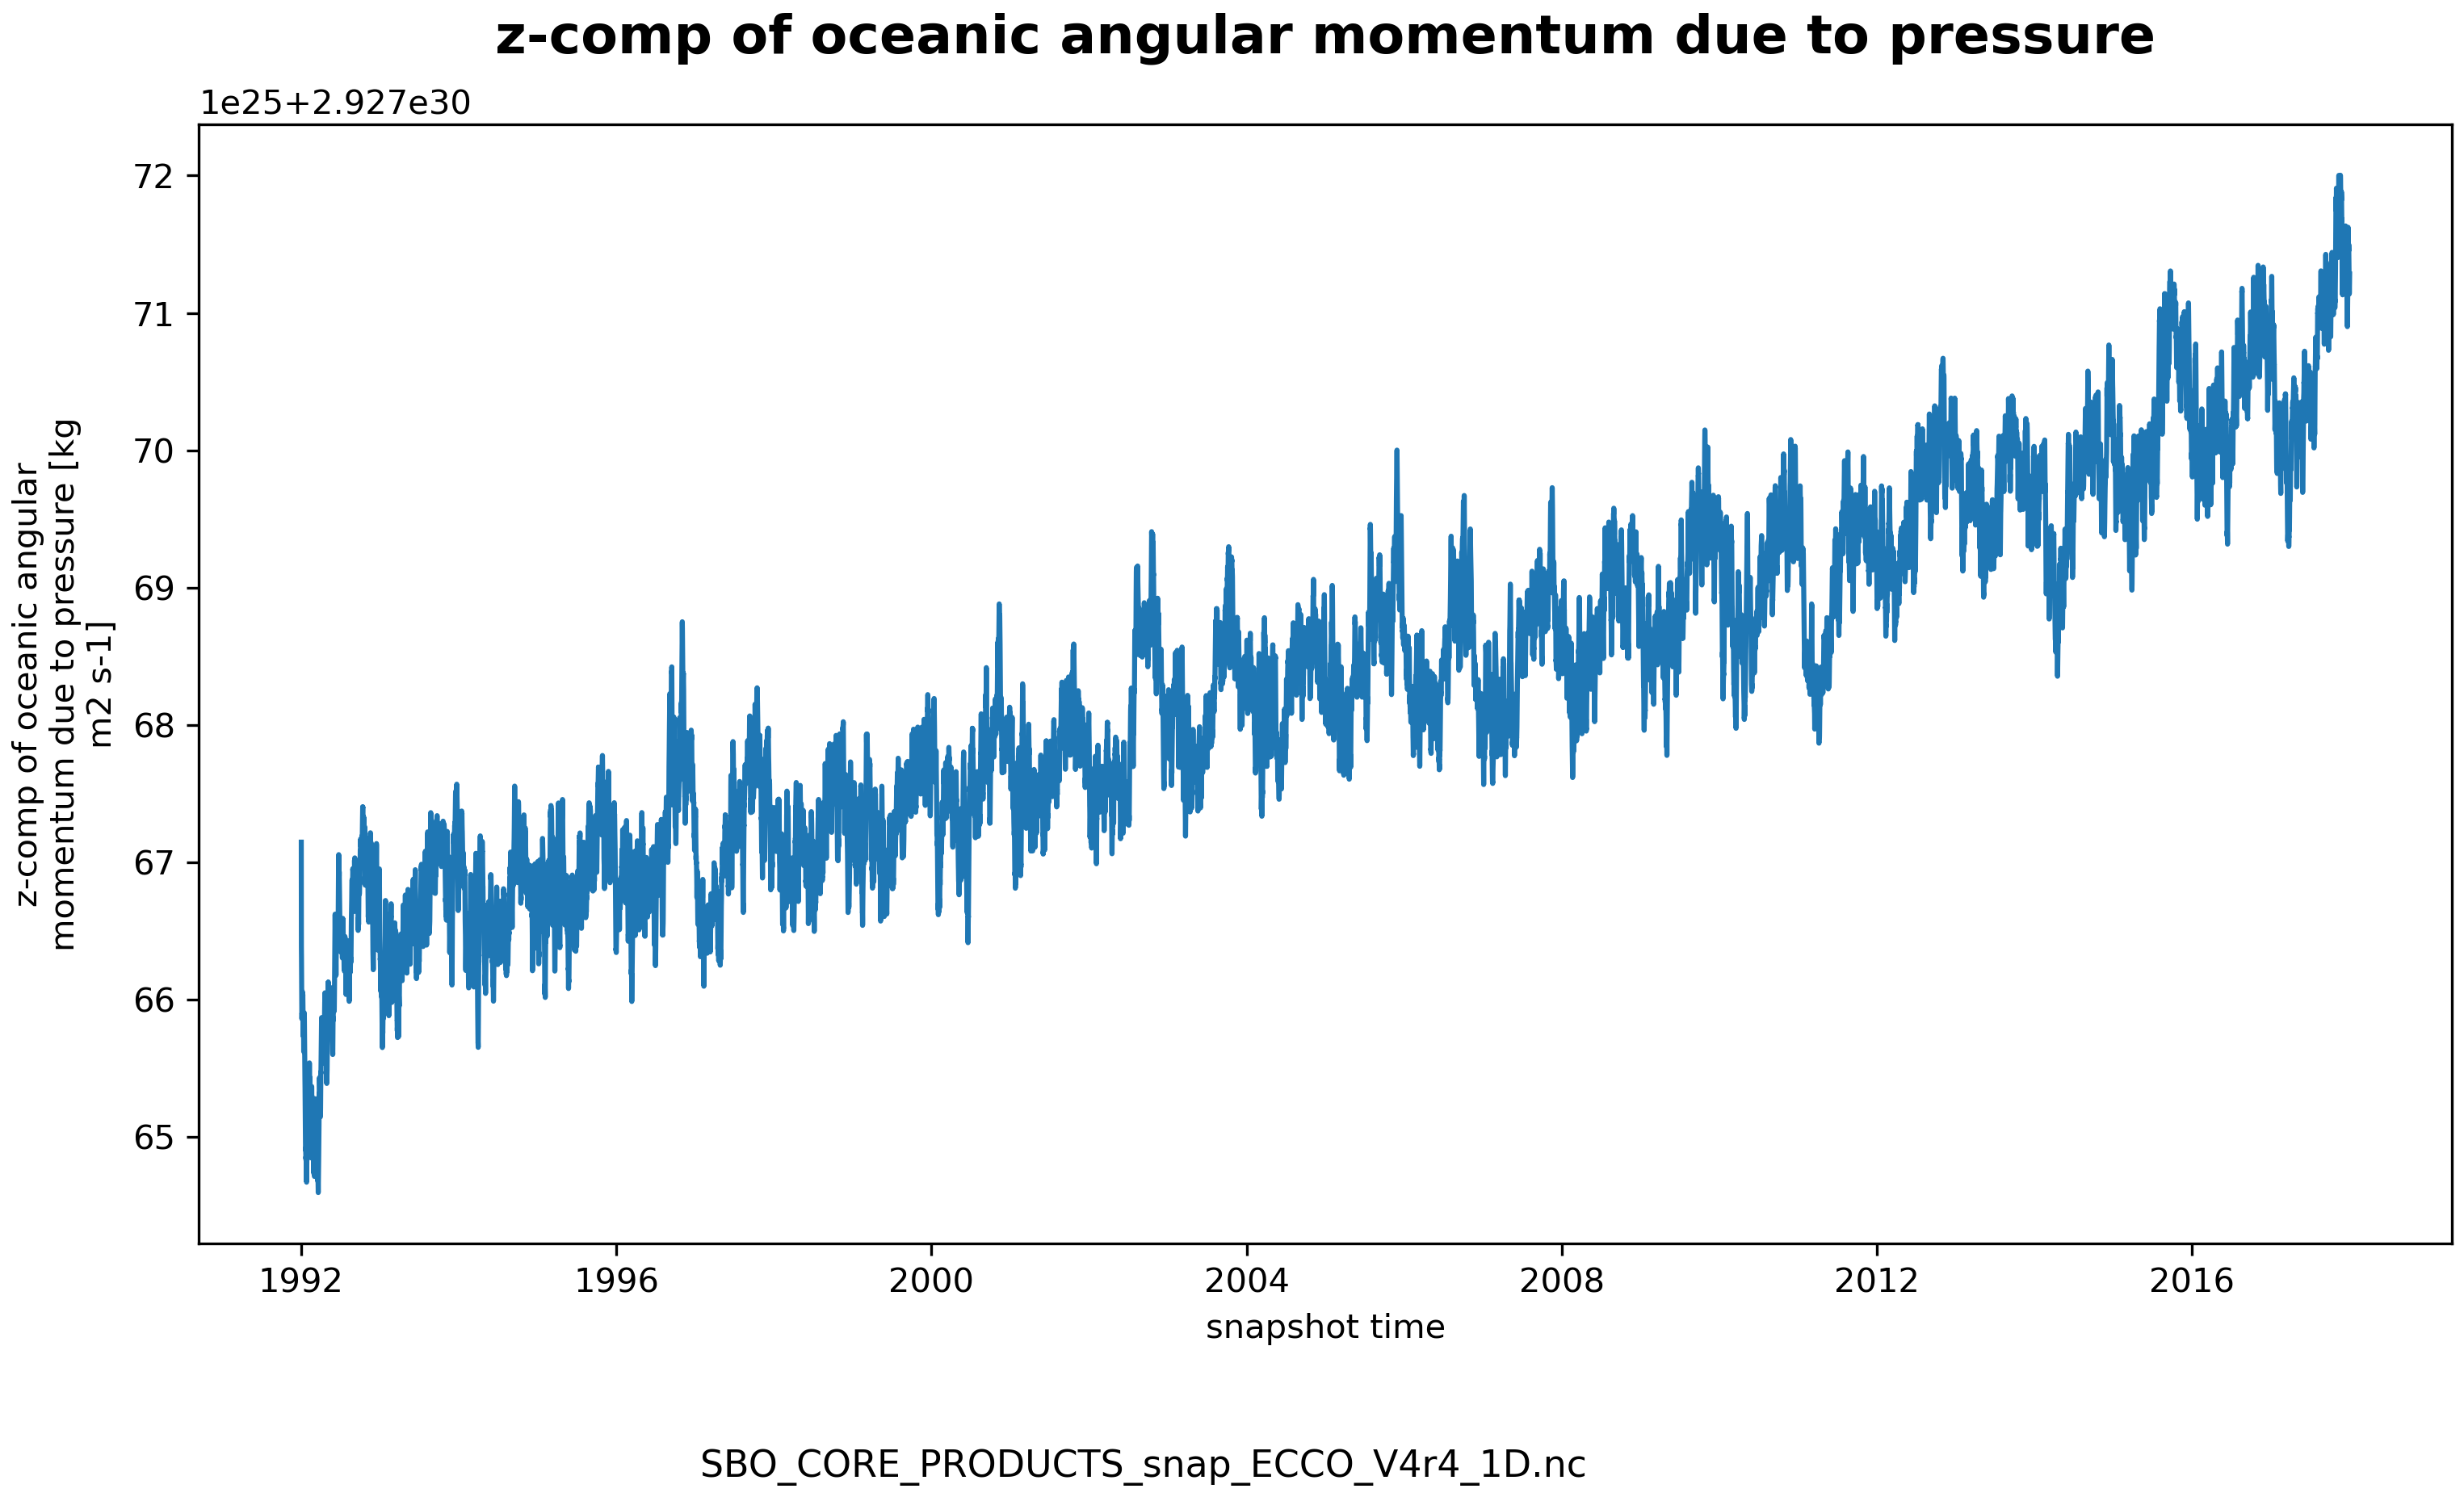
\includegraphics[scale=0.55]{../images/plots/v4r4/oneD_plots/SBO_Core_Products/zoamp.png}
\caption{Dataset: SBO\_CORE\_PRODUCTS, Variable: zoamp}
\label{tab:table-SBO_CORE_PRODUCTS_zoamp-Plot}
\end{figure}
\newpage
\pagebreak
\subsubsection{1D Variable: zoamp\_dsl}
\begin{longtable}{|m{0.06\textwidth}|m{0.3\textwidth}|m{0.45\textwidth}|m{0.12\textwidth}|}
\caption{Attributes description of the variable 'zoamp\_dsl' from SBO\_CORE\_PRODUCTS's  dataset.}
\label{tab:table-SBO_CORE_PRODUCTS_zoamp_dsl} \\ 
\hline \endhead \hline \endfoot
\rowcolor{lightgray} \textbf{Storage Type} & \textbf{Variable Name} & \textbf{Description} & \textbf{Unit} \\ \hline
float64 & zoamp\_dsl & Z-comp of oceanic angular momentum due to pressure based on dynamic (ib-corrected) sea level & kg m2 s-1 \\ \hline
\multicolumn{4}{|c|}{\cellcolor{lightgray}{\textbf{Description of the variable in Common Data language (CDL)}}} \\ \hline
\multicolumn{4}{|c|}{\fontfamily{lmtt}\selectfont{\makecell{\parbox{.95\textwidth}{\vspace*{0.25cm} \footnotesize{float64 zoamp\_dsl(time)\\
\hspace*{0.5cm}zoamp\_dsl: \_FillValue = 9.969209968386869e+36\\
\hspace*{0.5cm}zoamp\_dsl: coordinates = time\\
\hspace*{0.5cm}zoamp\_dsl: coverage\_content\_type = modelResult\\
\hspace*{0.5cm}zoamp\_dsl: long\_name = z-comp of oceanic angular momentum due to pressure based on dynamic (IB-corrected) sea level\\
\hspace*{0.5cm}zoamp\_dsl: units = kg m2 s-1\\
\hspace*{0.5cm}zoamp\_dsl: valid\_max = 2.9277328440911863e+30\\
\hspace*{0.5cm}zoamp\_dsl: valid\_min = 2.9276609546728614e+30\\
}}}}} \\ \hline
\rowcolor{lightgray} \multicolumn{4}{|c|}{\textbf{Comments}} \\ \hline
\multicolumn{4}{|p{1\textwidth}|}{\footnotesize{{N/a}}} \\ \hline
\end{longtable}

\begin{figure}[H]
\centering
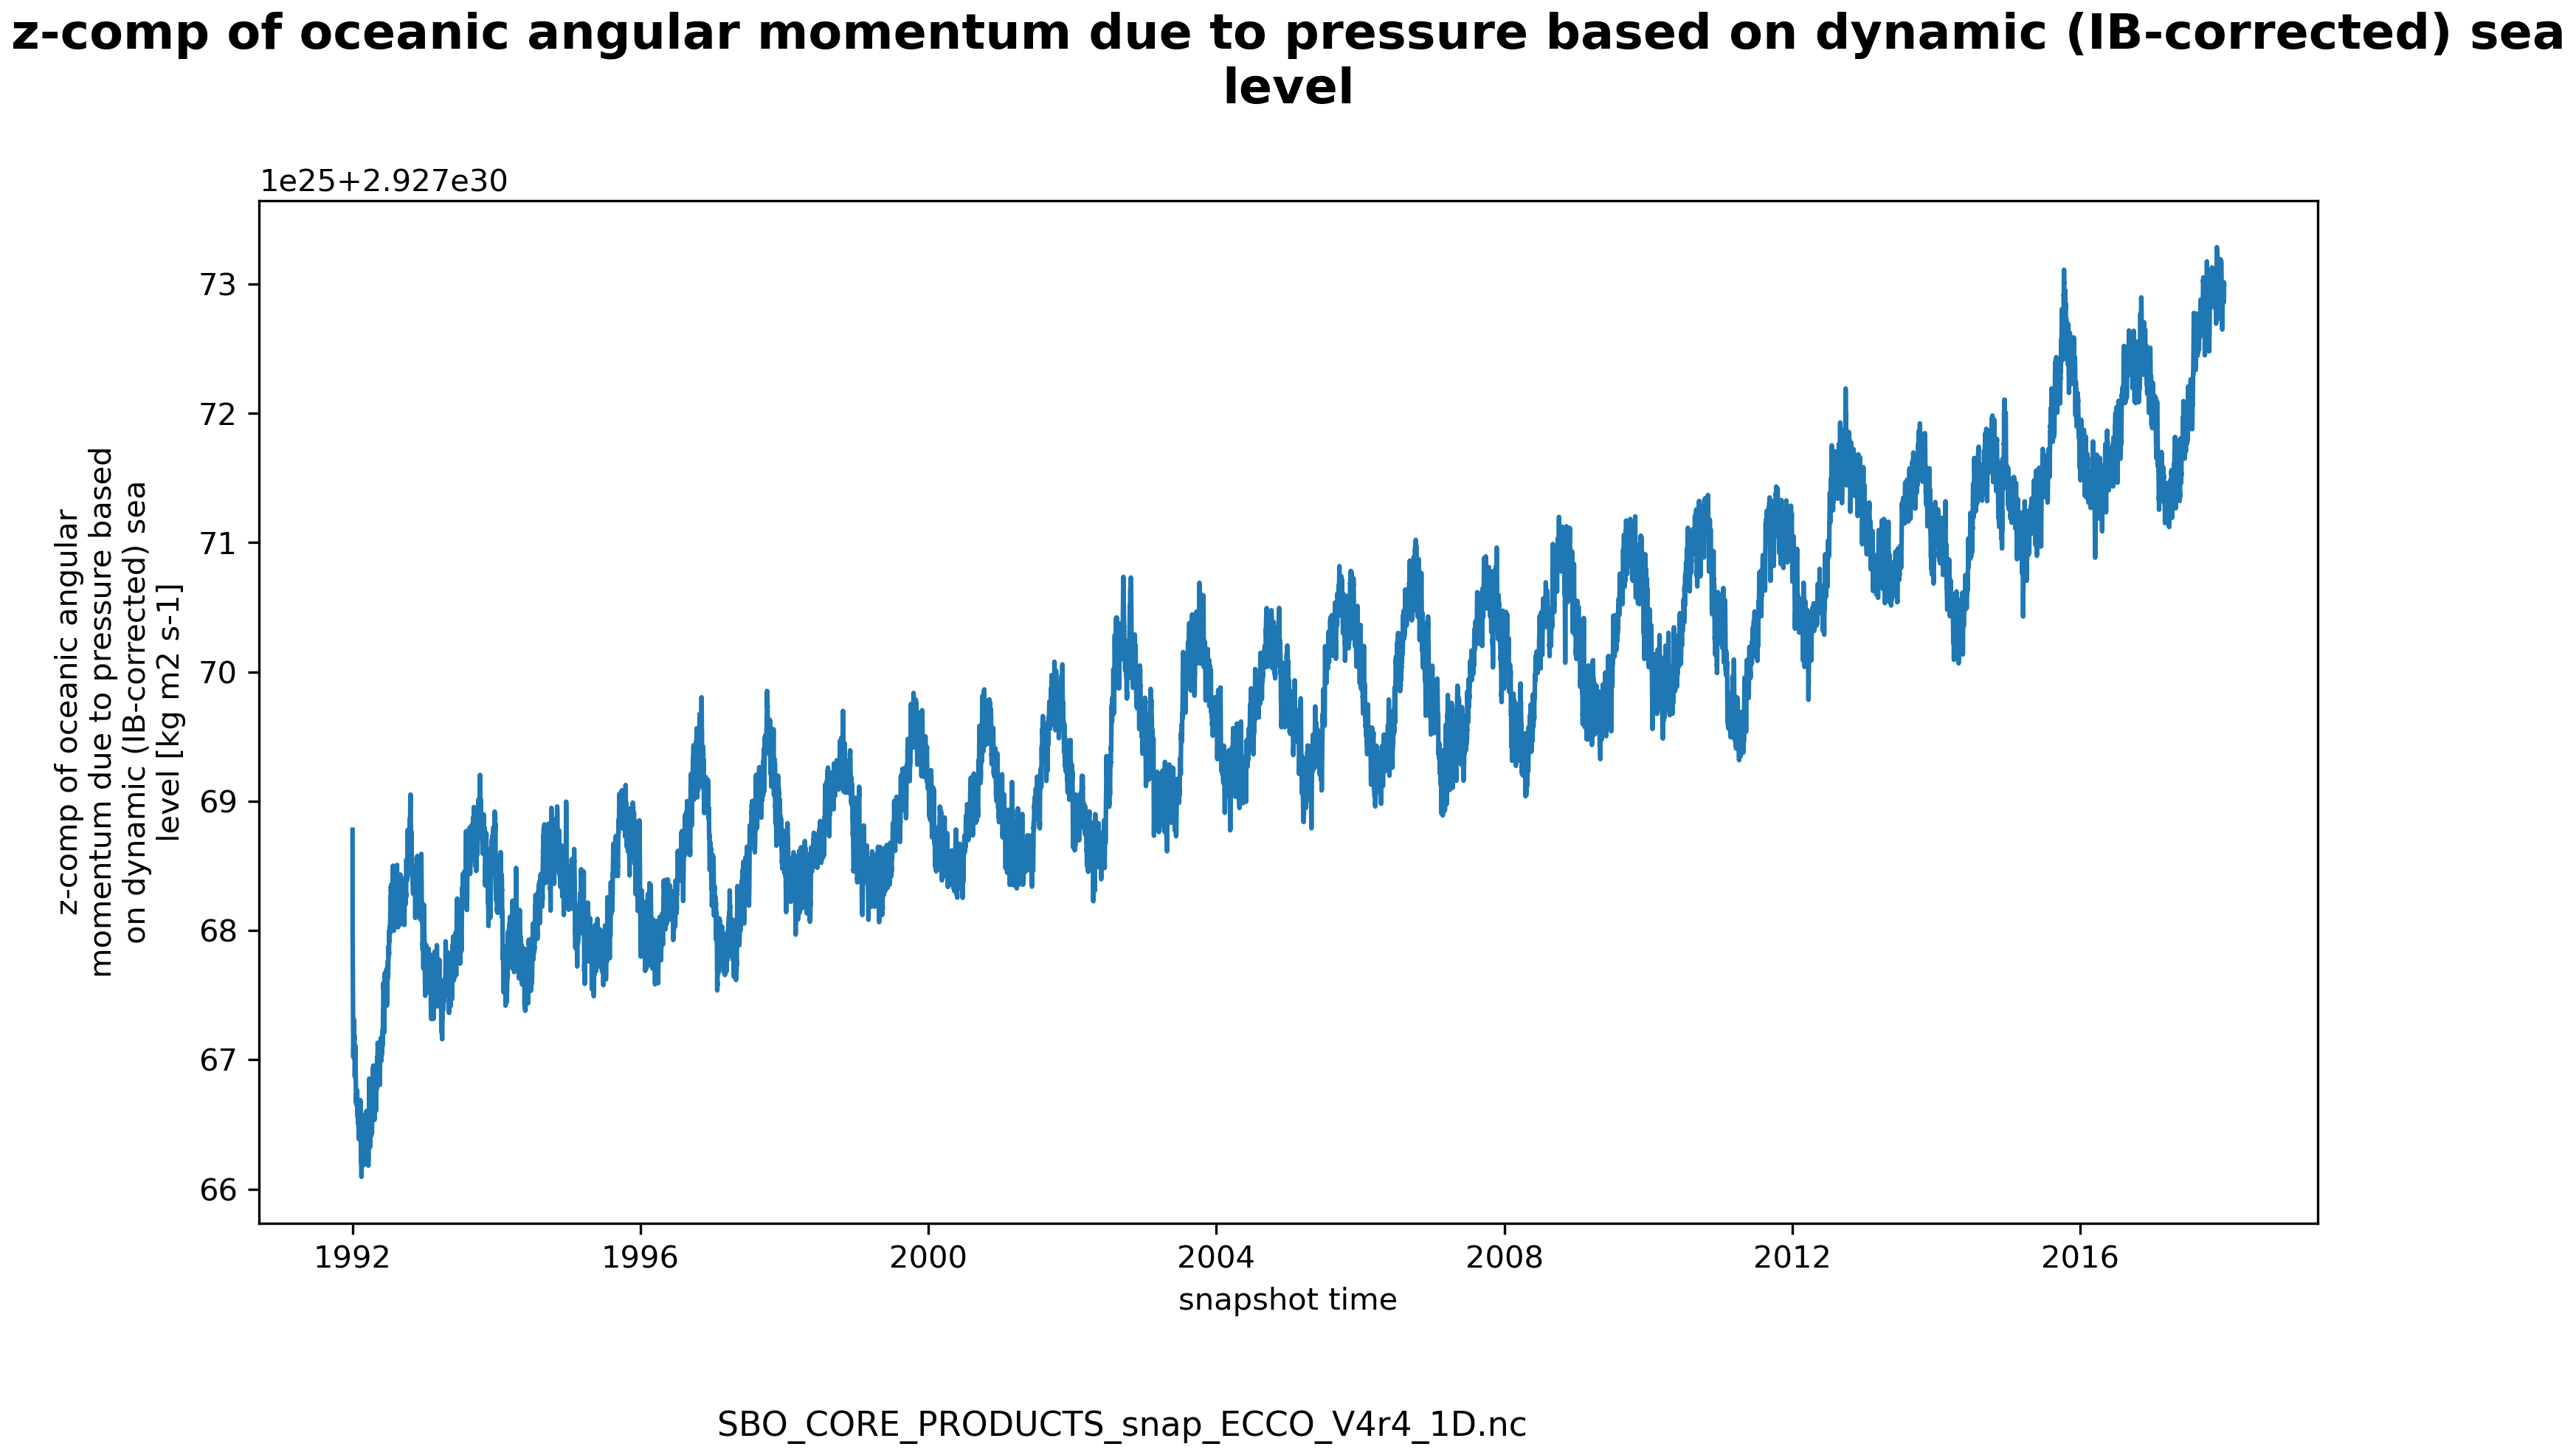
\includegraphics[scale=0.55]{../images/plots/v4r4/oneD_plots/SBO_Core_Products/zoamp_dsl.png}
\caption{Dataset: SBO\_CORE\_PRODUCTS, Variable: zoamp\_dsl}
\label{tab:table-SBO_CORE_PRODUCTS_zoamp_dsl-Plot}
\end{figure}
\newpage
\pagebreak
\subsubsection{1D Variable: zoamp\_fw}
\begin{longtable}{|m{0.06\textwidth}|m{0.3\textwidth}|m{0.45\textwidth}|m{0.12\textwidth}|}
\caption{Attributes description of the variable 'zoamp\_fw' from SBO\_CORE\_PRODUCTS's  dataset.}
\label{tab:table-SBO_CORE_PRODUCTS_zoamp_fw} \\ 
\hline \endhead \hline \endfoot
\rowcolor{lightgray} \textbf{Storage Type} & \textbf{Variable Name} & \textbf{Description} & \textbf{Unit} \\ \hline
float64 & zoamp\_fw & Z-comp of oceanic angular momentum due to freshwater flux & kg m2 s-1 \\ \hline
\multicolumn{4}{|c|}{\cellcolor{lightgray}{\textbf{Description of the variable in Common Data language (CDL)}}} \\ \hline
\multicolumn{4}{|c|}{\fontfamily{lmtt}\selectfont{\makecell{\parbox{.95\textwidth}{\vspace*{0.25cm} \footnotesize{float64 zoamp\_fw(time)\\
\hspace*{0.5cm}zoamp\_fw: \_FillValue = 9.969209968386869e+36\\
\hspace*{0.5cm}zoamp\_fw: coordinates = time\\
\hspace*{0.5cm}zoamp\_fw: coverage\_content\_type = modelResult\\
\hspace*{0.5cm}zoamp\_fw: long\_name = z-comp of oceanic angular momentum due to freshwater flux\\
\hspace*{0.5cm}zoamp\_fw: units = kg m2 s-1\\
\hspace*{0.5cm}zoamp\_fw: valid\_max = 1.442874536478883e+26\\
\hspace*{0.5cm}zoamp\_fw: valid\_min = 7.774584605728723e+25\\
}}}}} \\ \hline
\rowcolor{lightgray} \multicolumn{4}{|c|}{\textbf{Comments}} \\ \hline
\multicolumn{4}{|p{1\textwidth}|}{\footnotesize{{N/a}}} \\ \hline
\end{longtable}

\begin{figure}[H]
\centering
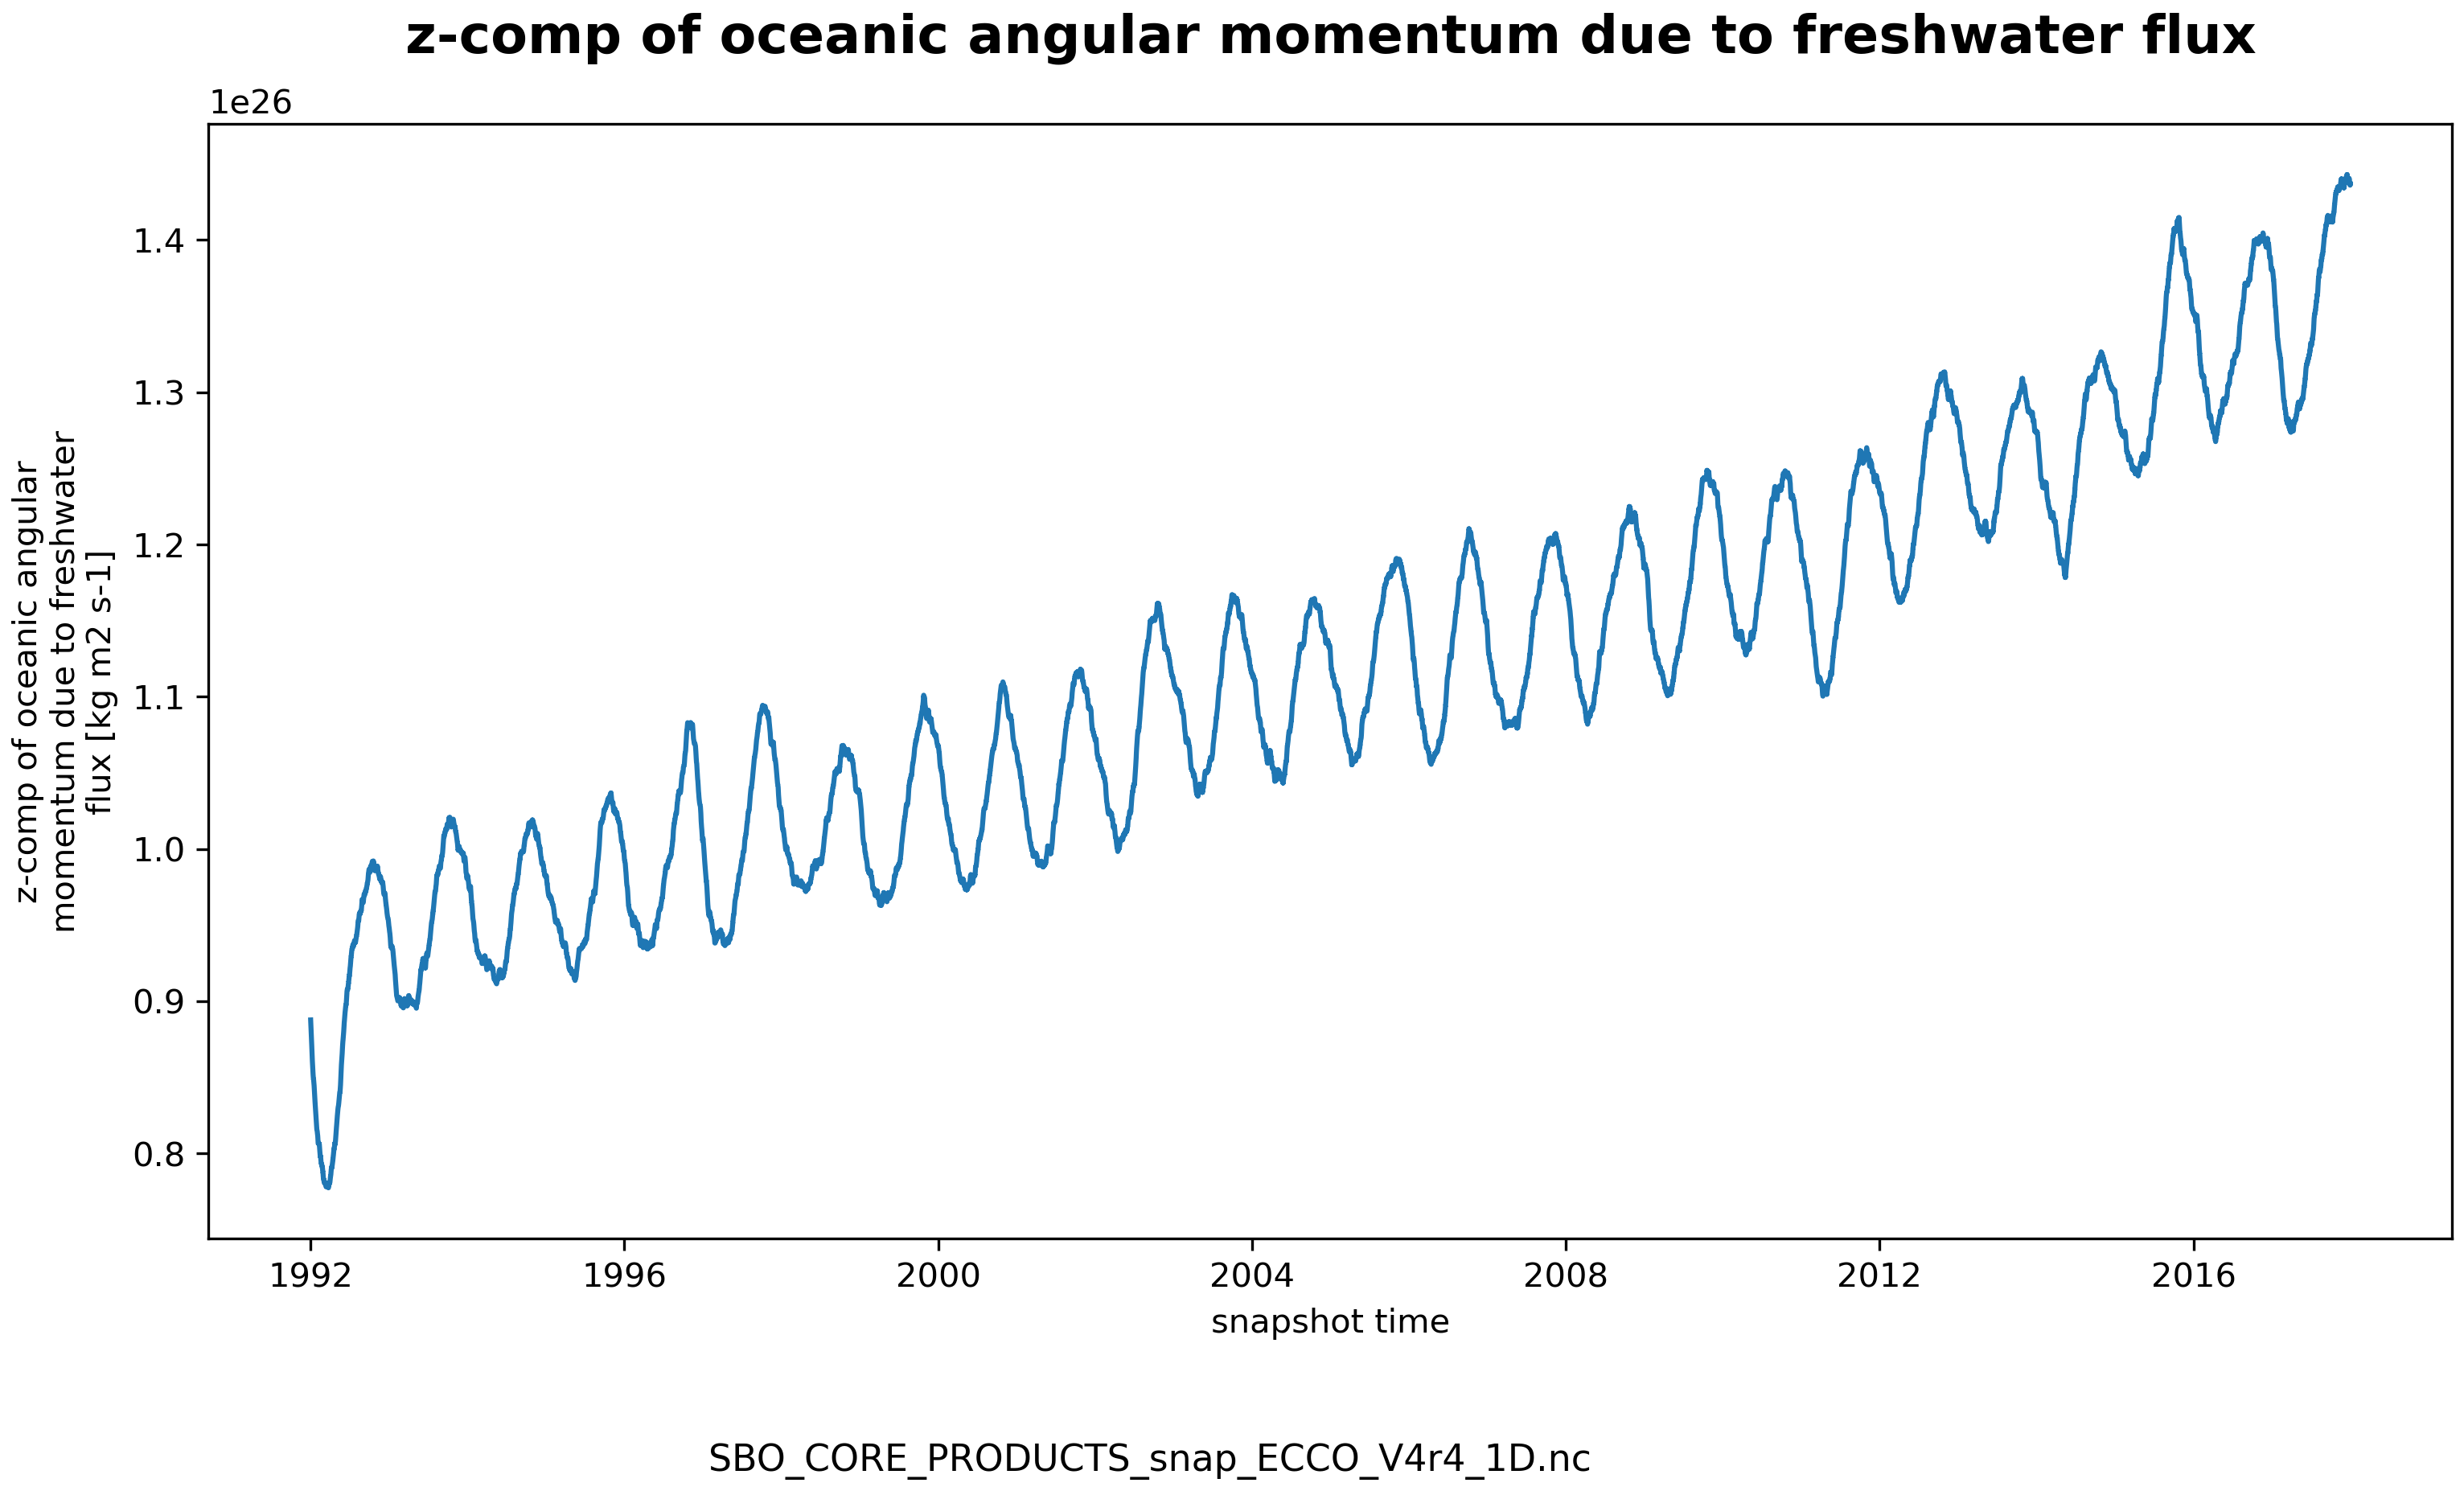
\includegraphics[scale=0.55]{../images/plots/v4r4/oneD_plots/SBO_Core_Products/zoamp_fw.png}
\caption{Dataset: SBO\_CORE\_PRODUCTS, Variable: zoamp\_fw}
\label{tab:table-SBO_CORE_PRODUCTS_zoamp_fw-Plot}
\end{figure}
\newpage